% Options for packages loaded elsewhere
\PassOptionsToPackage{unicode}{hyperref}
\PassOptionsToPackage{hyphens}{url}
%
\documentclass[
]{article}
\usepackage{lmodern}
\usepackage{amssymb,amsmath}
\usepackage{ifxetex,ifluatex}
\ifnum 0\ifxetex 1\fi\ifluatex 1\fi=0 % if pdftex
  \usepackage[T1]{fontenc}
  \usepackage[utf8]{inputenc}
  \usepackage{textcomp} % provide euro and other symbols
\else % if luatex or xetex
  \usepackage{unicode-math}
  \defaultfontfeatures{Scale=MatchLowercase}
  \defaultfontfeatures[\rmfamily]{Ligatures=TeX,Scale=1}
\fi
% Use upquote if available, for straight quotes in verbatim environments
\IfFileExists{upquote.sty}{\usepackage{upquote}}{}
\IfFileExists{microtype.sty}{% use microtype if available
  \usepackage[]{microtype}
  \UseMicrotypeSet[protrusion]{basicmath} % disable protrusion for tt fonts
}{}
\makeatletter
\@ifundefined{KOMAClassName}{% if non-KOMA class
  \IfFileExists{parskip.sty}{%
    \usepackage{parskip}
  }{% else
    \setlength{\parindent}{0pt}
    \setlength{\parskip}{6pt plus 2pt minus 1pt}}
}{% if KOMA class
  \KOMAoptions{parskip=half}}
\makeatother
\usepackage{xcolor}
\IfFileExists{xurl.sty}{\usepackage{xurl}}{} % add URL line breaks if available
\IfFileExists{bookmark.sty}{\usepackage{bookmark}}{\usepackage{hyperref}}
\hypersetup{
  pdftitle={Bounds in Two-Sample Mendelian Randomization With Summary Statistics},
  hidelinks,
  pdfcreator={LaTeX via pandoc}}
\urlstyle{same} % disable monospaced font for URLs
\usepackage[margin=1in]{geometry}
\usepackage{longtable,booktabs}
% Correct order of tables after \paragraph or \subparagraph
\usepackage{etoolbox}
\makeatletter
\patchcmd\longtable{\par}{\if@noskipsec\mbox{}\fi\par}{}{}
\makeatother
% Allow footnotes in longtable head/foot
\IfFileExists{footnotehyper.sty}{\usepackage{footnotehyper}}{\usepackage{footnote}}
\makesavenoteenv{longtable}
\usepackage{graphicx}
\makeatletter
\def\maxwidth{\ifdim\Gin@nat@width>\linewidth\linewidth\else\Gin@nat@width\fi}
\def\maxheight{\ifdim\Gin@nat@height>\textheight\textheight\else\Gin@nat@height\fi}
\makeatother
% Scale images if necessary, so that they will not overflow the page
% margins by default, and it is still possible to overwrite the defaults
% using explicit options in \includegraphics[width, height, ...]{}
\setkeys{Gin}{width=\maxwidth,height=\maxheight,keepaspectratio}
% Set default figure placement to htbp
\makeatletter
\def\fps@figure{htbp}
\makeatother
\setlength{\emergencystretch}{3em} % prevent overfull lines
\providecommand{\tightlist}{%
  \setlength{\itemsep}{0pt}\setlength{\parskip}{0pt}}
\setcounter{secnumdepth}{5}
\usepackage{amsmath,amsfonts,amssymb,amsthm}
\usepackage{tikz}
\usetikzlibrary{positioning}

\usepackage{longtable}
\usepackage{booktabs}
\usepackage{caption}
\usepackage{subcaption}
\usepackage{rotating}
\usepackage{float}
\theoremstyle{plain}
\newtheorem{theorem}{Theorem}[section]
\newtheorem{corollary}[theorem]{Corollary}
\usepackage{booktabs}
\usepackage{longtable}
\usepackage{array}
\usepackage{multirow}
\usepackage{wrapfig}
\usepackage{float}
\usepackage{colortbl}
\usepackage{pdflscape}
\usepackage{tabu}
\usepackage{threeparttable}
\usepackage{threeparttablex}
\usepackage[normalem]{ulem}
\usepackage{makecell}
\usepackage{xcolor}
\ifluatex
  \usepackage{selnolig}  % disable illegal ligatures
\fi
\usepackage[]{natbib}
\bibliographystyle{plainnat}

\title{Bounds in Two-Sample Mendelian Randomization With Summary Statistics}
\author{}
\date{\vspace{-2.5em}}

\begin{document}
\maketitle

{
\setcounter{tocdepth}{2}
\tableofcontents
}
\newpage

\hypertarget{introduction}{%
\section{Introduction}\label{introduction}}

The gold standard to estimate the causal effect of a treatment or an exposure on an outcome is a randomized trial where the treatment assignment is randomized. However, in many epidemiological studies, randomized experiments are not feasible. For example, a study estimating the negative effects of smoking on depression \citep{wootton_evidence_2019} would not be feasible with a randomized trial due to ethical concerns. In such settings, epidemiologists rely on different types of observational studies, which introduces potential biases from unmeasured confounders. In recent years, there has been an increase in using instrumental variable (IV) in the form of Mendelian randomization (MR) \citep{davey_smith_mendelian_2003, lawlor_mendelian_2008}. Briefly, IV is a variable that is (A1) associated with the exposure, (A2) is independent from unmeasured confounders affecting the exposure and the outcome, and (A3) affects the outcome only through its effect on the exposure; see \ref{sec:iv-assumptions-and-two-sample-mr} for details. MR uses genetic variants, usually single nucleotide polymorphisms, as instruments to estimate the causal effect of an exposure on an outcome. This is based on the idea being that genotypes are randomly assigned when passed on from parents to offspring at meiosis \citep{lawlor_mendelian_2008} and thus, they make excellent candidates for satisfying (A2), especially when the exposure of interest is environmental.

MR analyses often use published summary statistics from two independent genome wide association studies \citep{burgess_mendelian_2013, burgess_using_2015, davies_reading_2018} \textcolor{red}{Not sure about these citations...we can discuss(Erlich and Narayanan 2014; Fuller et al. 1999; Wang et al. 2017)}. Typically, the first study provides information about the exposure and instrument and the second study provides information about the outcome and instrument. Once investigator have summary statistics from two studies, they use methods based on parametric modeling assumptions \citep{burgess_mendelian_2015, burgess_review_2017} to arrive at point estimates and tests for the exposure effect.

An alternative approach to study the casual effect of the exposure without parametric assumptions is through non-parametric IV bounds \citep{balke_bounds_1997, cheng_bounds_2006, manski_nonparametric_1990, richardson_ace_2014, robins_analysis_1989}. Briefly, nonparametric IV bounds only use the bare minimum amount of assumptions, usually (A1)-(A3), to provide a range of plausible values for the exposure effect. They are typically used when the outcome, the exposure, and the instrument are all binary and are simultaneously observed. The most well-known are the Balke-Pearl bounds for the average treatment effect under slight variants of assumptions (A1)-(A3), and a set of instrumental inequalities to falsify the IV assumptions. Since then, \citet{cheng_bounds_2006} and \citet{richardson_ace_2014} extended the Balke-Pearl bounds to allow for a non-binary instrument. \citet{ramsahai_causal_2012} derived bounds for the two-sample setting where the exposure and instrument are observed from one study and the outcome and instrument are observed from another study. \citet{bpbounds-package} provides software to compute IV bounds for two-sample MR studies using only summary statistics. For a recent overview, see Swanson et al.~(2018).

Due to their nonparametric nature, the IV bounds are attractive approaches to analyze exposure effects especially if some modeling assumptions are suspect or difficult to justify. In MR, the minimal set of assumptions needed for non-parametric bounds is a stark contrast to many other MR approaches, such as the IVW estimator \citep{burgess_mendelian_2013}, MR-Egger regression \citep{bowden_assessing_2016}, weighted median \citep{bowden_consistent_2016} and modes \citep{hartwig_robust_2017}, MRRAPs \citep{zhao_statistical_2020}, and others, that make parametric assumptions about the exposure effect. More generally, if IV bounds using fewer assumptions arrive at similar conclusions about the exposure effect as those based on parametric approaches, the case for the causal effect on the exposure becomes stronger.

Despite their attractive properties, there is a poor understanding about the behavior of IV bounds in two-sample MR studies using only summary statistics. The specific questions we will tackle in our work are

\begin{enumerate}
\item What kind of genetic instruments are needed to provide useful conclusions about the exposure effect, say the bound does not contain the null effect?
\item Can combining multiple instruments lead to shorter and tighter bounds on the exposure effect? 
\item How do the bounds change if many instruments are weak, which is typically the case in MR studies based on genetic instruments? 
\end{enumerate}

In traditional setups for IV bounds where individual-level data consisting jointly of the outcome, the exposure, and a single instrument are available, the Balke-Pearl bounds are usually conservative and contain the null effect. However, it is not clear if the same principle holds for two-sample MR studies, especially if multiple candidate IVs are available. The goal of the paper is to address these questions and provide a more in-depth exploration of these bounds, specifically addressing what we can expect to learn and what information can be gained by utilizing multiple IVs under assumptions similar to Balke-Pearl bounds

The paper is divided as follows. Section \ref{} \textcolor{red}{Fill this after done}.

\hypertarget{setup}{%
\section{Setup}\label{setup}}

\hypertarget{review-notation-and-definitions}{%
\subsection{Review: Notation and Definitions}\label{review-notation-and-definitions}}

\label{notation-and-definitions}

In the following, let \(X\) and \(Y\) be binary exposure and outcome, respectively, \(Z\) be a categorical instrumental variable taking values in \{0, 1, and 2\}, and \(U\) an unmeasured confounder for the effect of \(X\) on \(Y\). No assumptions about the structure of \(U\) are made. Let \(Y^{z,x}\) be the potential outcome \citep{rubin_estimating_1974, splawa-neyman_application_1990} had the subject received exposure value \(X = x\) and instrument value \(Z = z\). Throughout the paper, we assume the stable unit treatment value assumption (SUTVA) \citep{cox_planning_1958, rubin_randomization_1980}, formalized as \(Y = \sum_{x,z} I[Z = z, X = x] Y^{x,z}\) and \(I[\cdot]\) is the indicator function.

We make the following set of assumptions about the instrument, the exposure, the outcome, and the unmeasured confounder that are typical in MR studies; see \citet{didelez_mendelian_2007} and \citet{wang_bounded_2018} for details

\begin{itemize}
\tightlist
\item[(A1)] \emph{(Relevance)}: $Z \not\perp X$ 
\item[(A2)] \emph{(Independent instrument)}: $Z \perp U$
\item[(A3)] \emph{(Exclusion restriction)}: $Y^{z,x} = Y^{z',x} = Y^{x}$ for all $x,z,z'$
\item[(A4)] \emph{(Conditional ignorability of $X,Z$ given $U$)}: $Y^{z,x} \perp Z, X | U$
\end{itemize}

Briefly, assumption (A1) can be assessed by finding SNPs that have been consistently associated with the exposure through multiple GWAS (Marigorta et al.~2018). Assumption (A2) is usually checked based on scientific theory surrounding how the genetic instrument was inherited from the parents to the offspring. Assumption (A3) states that there is no direct effect of the instrument \(Z\) on the outcome \(Y\) other than that through the exposure \(X\) and like assumption (A2), is assessed by scientific theory. Both assumptions (A2) and (A3) can be violated if the SNP is (i) in linkage disequilibrium with an unmeasured SNP that affects the exposure and outcome, (ii) pleiotropic and has multiple functions beyond affecting the exposure, or (iii) under population stratification, to name a few. For a more in-depth discussion of (A1)-(A3) in MR studies, see \citet{lawlor_mendelian_2008}. Finally (A4) states that if \(U\) is observed, then it is sufficient to unconfound the relationship between \(X\) and \(Y\).

We make a few additional remarks about assumptions (A1)-(A4). First, most MR studies only make assumptions (A1)-(A3) along with some modeling assumptions \textcolor{red}{Cite MR book}\textcolor{blue}{ RMT:  The burgess and Thompson book?}. Second, the role of assumption (A4) is to mainly show the role that an unmeasured confounder \(U\) plays in potentially allowing identification of the causal effect of the treatment if it were measured; \citet{richardson_ace_2014} showed that one can remove (A4) and strengthen (A2) with \(Z \perp U, Y^{z,x}\) and arrive at the same IV bounds of Balke and Pearl. Third, under SUTVA and assumptions (A3)-(A4), we have \(Y \perp Z | X, U\), which is another common way to express the exclusion restriction in MR studies \citep{didelez_mendelian_2007}. Fourth, for simplicity, we do not assume the the existence of a potential treatment \(X^{z}\); the existence of \(X^z\) does not change the IV bounds \citep{swanson_partial_2018, richardson_ace_2014}, and its primarily purpose is to define a ``causal'' instrument \citep{hernn_instruments_2006}.

We conclude by introducing two assumptions and defining instrument strength; the assumptions are not necessarily to construct bounds, but will help us explain the behavior of the IV bounds. First, we state the assumptions restricting the direction of the instrument's effect on the exposure and the outcome.

\begin{itemize}
\item[(A5)] \emph{(Monotonicity between $Z$ and $X$)} $P(X = 1 | Z = z, U) \le P(X = 1 | Z = z+1, U)$ for $z=0,1$
\item[(A6)] \emph{(Monotonicity between $Z$ and $Y$)} $P(Y = 1 | Z = z, U) \le P(Y = 1 | Z = z+1, U)$ for $z=0,1$
\end{itemize}

A variant of assumption (A5) is common in the IV literature to study noncompliance \citep{angrist_identification_1996, baiocchi_instrumental_2014}. Assumption (A6) is an extension of assumption (A5) to the outcome variable. Assumptions (A5) or (A6) is plausible in MR if the direction of the effects of the genetic instrument on the exposure or the outcome are well-established from scientific theory and replication of findings from many observational studies.

Second, we define instrument strength as the maximum possible contrast between the exposure when instruments take on different values

\begin{equation}
\text{ST} = \max_{z_1 \neq z_2} | P(X = 1 | Z = z_1) - P(X = 1 | Z = z_2) | \label{eq:strength}
\end{equation}

ST matches the definition of instrument strength used in Balke and Pearl \textcolor{red}{cite year} \textcolor{blue}{ RMT: not sure where they mention strength} when the instrument is binary; in that work, it was used to justify how the width of the IV bounds changed as a function of \(\text{ST}\). However, \eqref{eq:strength} differs from other definitions of strength based on a parametric model between the exposure and the outcome, say the concentration parameter; \citet{stock_survey_2002} for an overview.

\hypertarget{review-study-designs-and-target-estimand}{%
\subsection{Review: Study Designs and Target Estimand}\label{review-study-designs-and-target-estimand}}

There are roughly two designs of IV studies, the two-sample design and the one-sample design. The two-sample design has two separate data sources, one providing information of \((X,Z)\) and one providing information of \((Y,Z)\), and is the most popular design in MR studies. The one-sample design has a single data source providing information on all observed variables \((X,Y,Z)\) and is more common in traditional IV studies involving non-genetic instruments. Also, the behavior of bounds under a one-sample design has been well-studied more extensively than in two-sample design \citep{swanson_partial_2018}.

In a MR study under a two-sample design, investigators often rely on summary statistics from GWAS to study the exposure effect. When both the outcome and the exposure are binary as is the case for case-control study, these summary statistics are computed by running a logistic regression between the exposure \(X\) and the outcome \(Y\) for each genetic instrument \(Z\) and extracting the estimated slope coefficients associated with \(Z\); \textcolor{blue}{ RMT: here it sounds like these are log reg for one at a time in contrast to multiple log reg. Is that the case?} it's also common for the logistic regression to adjust for age, sex, and principal components. To focus our paper on studying behavior of bounds not due to sampling errors, we will assume that we have population-level quantities \(P(Y = 1 | Z = z)\) from one data source and \(P(X = 1 | Z = z)\) from another data source for different values of \(z\).

The focus of the paper is on the average treatment effect (ATE)

\[
\text{ATE} = E[Y^1 - Y^0] = \int P(Y=1 \mid X = 1, U=u) P(U=u) du - \int P(Y=1 \mid X = 0, U=u) P(U=u) du, 
\]

where the second equality follows from SUTVA and assumptions (A3)-(A4). Since \(U\) is not observed, additional assumptions are needed to point-identify the ATE. In particular, even with the remaining assumptions (A1), (A2), and (A5), the ATE cannot be point-identified; see \citet{robins_analysis_1989}, \citet{manski_nonparametric_1990}, and \citet{balke_counterfactuals_1995}.

In one-sample designs, sharp bounds on the ATE are well-established under assumptions (A1)-(A4) \citep{balke_bounds_1997, richardson_ace_2014, swanson_partial_2018}; these bounds can also be used when individual-level data are not available, but population summary statistics in the form of \(P(Y = y, X = x | Z = z)\) for \(y,x,z\) are known. In two-sample designs, \citet{ramsahai_causal_2012} showed that under assumptions (A1)-(A4), the bounds for the ATE are

\[
\begin{aligned}
\max &\left \{
\begin{array}{ll}
  \max_{z_1 \neq z_2} & P(Y = 1 | Z = z_1) - 2\cdot P(Y = 1 | Z = z_2) - 2\cdot P(X = 1 | Z = z_2) \\
  \max_{z_1 \neq z_2} & P(Y = 1 | Z = z_1) + P(X = 1 | Z = z_1) - P(Y = 1 | Z = z_2) - P(X = 1 | Z = z_2) - 1 \\
  \max_{z_1 \neq z_2} & 2\cdot P(Y = 1 | Z = z_1) + 2\cdot P(X = 1 | Z = z_1) - P(Y = 1 | Z = z_2) - 3 \\
  \max_z & -P(Y = 1 | Z = z) - P(X = 1 | Z = z) \\
  \max_z & P(Y = 1 | Z = z) +  P(X = 1 | Z = z) - 2
\end{array}
\right \} \\ \\
& \qquad \qquad \qquad \qquad \le ATE \le \\ \\
& \qquad \quad \min \left \{
\begin{array}{ll}
  \min_{z_1 \neq z_2} & P(Y = 1 | Z = z_1) - 2\cdot P(Y = 1 | Z = z_2) +  2\cdot P(X = 1 | Z = z_2) + 1 \\
  \min_{z_1 \neq z_2} & P(Y = 1 | Z = z_1) + 2\cdot P(Y = 1 | Z = z_2) -  2\cdot P(X = 1 | Z = z_2) + 1 \\
  \min_{z_1 \neq z_2} & P(Y = 1 | Z = z_1) - P(X = 1 | Z = z_1) + P(X = 1 | Z = z_2) - P(Y = 1 | Z = z_2) + 1 \\
  \min_z & P(X = 1 | Z = z) - P(Y = 1 | Z = z) + 1 \\
  \min_z & P(Y = 1 | Z = z) - P(X = 1 | Z = z) + 1 
\end{array} 
\right \} \label{eq:ate_bound}
\end{aligned}
\]

Additionally, the data from two-sample designs can be used to check the validity of the assumptions

\begin{equation}
\min \left\{
  \begin{array}{ll}
    \min_{z_1 \neq z_2} & P(Y = 1 | Z = z_1) - P(X = 1 | Z = z_1) - P(Y = 1 | Z = z_2) - P(X = 1 | Z = z_2) + 2 \\
    \min_{z_1 \neq z_2} & P(Y = 1 | Z = z_1) + P(X = 1 | Z = z_1) - P(Y = 1 | Z = z_2) + P(X = 1 | Z = z_2) \\
    \min_{z} & P(X = 1 | Z = z) \\
    \min_{z} & P(Y = 1 | Z = z) \\
    \min_{z} & 1 - P(X = 1 | Z = z) \\
    \min_{z} & 1 - P(Y = 1 | Z = z) 
  \end{array} 
\right \} \ge 0 \label{eq:constraints}
\end{equation}

The inequalities in equation \eqref{eq:constraints} are extensions of the ``IV inequalities'' of \citet{balke_bounds_1997} used to check the validity of the IV assumptions. Versions of these inequalities have been used in MR studies \citep{diemer_application_2020} to check whether the genetic variants satisfy the IV assumptions. In the Appendix, we provide some details on deriving equations \eqref{eq:ate_bound} and \eqref{eq:constraints} as well as implementing the procedure using Polymake \citep{assarf_computing_2017}, a linear program solver in R. We also discuss a minor, but important numerical issue concerning ordering of the bounds; we believe this issue is pertinent among investigators who are using a linear-program based software to compute these bounds \citep{palmer_nonparametric_2011}. \textcolor{blue}{ RMT: Bounds from Richardson and Robins 2014 agree with these, and therefore also result in LB > UB every now and then. Not sure how they derive their expression, though...}

\hypertarget{properties-of-bounds-from-summary-level-data}{%
\section{Properties of Bounds from Summary-Level Data}\label{properties-of-bounds-from-summary-level-data}}

\hypertarget{bounds-from-bivariate-data}{%
\subsection{Bounds from Bivariate Data}\label{bounds-from-bivariate-data}}

We begin our investigation of bounds in equation \eqref{eq:ate_bound} under two-sample MR studies with summary data when there is a single instrument. We are interested in whether we can gain any insights into the direction and magnitude of the ATE by examining the length of the bounds; wide bounds provide less information about the magnitude of the ATE, and are much less likely to provide any information regarding direction as compared to narrower bounds.

Theorem \ref{thm:uppderBoundWidth} shows the width of the ATE bound in equation \eqref{eq:ate_bound} under a near-ideal MR study where all the assumptions (A1)-(A6) hold; in addition to having some evidence in support of assumptions (A1)-(A4) that are needed to obtain the bound in equation \eqref{eq:ate_bound}, the investigator knows that the genetic instrument has a monotonic effect on the exposure and the outcome for every value of the unmeasured value. Theoretically, the extra assumptions (A5)-(A6) simplify the bound formula in equation \eqref{eq:ate_bound}, allowing us to precisely characterize the width of the min/max inequalities.

\begin{theorem}\label{thm:upperBoundWidth}
Under assumptions (A1)-(A6), the bounds for the ATE in \eqref{eq:ate_bound} become

\[
  \begin{aligned}
    &\max
      \begin{Bmatrix}
        -P(Y = 0 | Z = 2) - P(Y = 1 | Z = 0) + P(X = 0 | Z = 0) - P(X = 0 | Z = 2) \\
        P(Y = 0 | Z = 0) - 2\cdot P(Y = 0 | Z = 2) - P(X = 0 | Z = 2) \\
        -P(Y = 0 | Z = 2) - 2\cdot P(Y = 1 | Z = 0) + P(X = 0 | Z = 0)
      \end{Bmatrix} \\
    &\qquad \qquad \qquad \qquad \qquad\le ATE \le \\
    &\qquad \qquad \qquad \min
      \begin{Bmatrix}
        1 + P(Y = 0 | Z = 0) - P(X = 0 | Z = 0) \\
        1 + P(Y = 0 | Z = 0) - P(Y = 0 | Z = 2) - P(X = 0 | Z = 0) + P(X = 0 | Z = 2) \\
        1 - P(Y = 0 | Z = 2) +  P(X = 0 | Z = 2)
      \end{Bmatrix}
  \end{aligned}
\]

and the width of the above bounds is bounded from above by $2 - 2\cdot \text{ST}$. \textcolor{red}{is this upper bound sharp when (A1)-(A6) hold? That is, there exists a DGP that satisfy (A1)-(A6) and the width of the bound from it is equal to the upper bound?}\textcolor{blue}{ RMT: Yes. I did construct a DGP artificially that gave width 2, but we also have lots of examples from the simulation of DGPs that hit the 2 - 2 ST line. I just checked, and 31 of those also satisfy the monotonicity assumptions.}
\end{theorem}

The proof is presented in Appendix \ref{proof-of-theorem}. The bounds under the near-ideal MR setting is \textcolor{blue}{ RMT: up to (?)} twice as large as the Balke-Pearl bounds with a binary IV in single-sample designs where the width is \(1-\text{ST}\). An instrument with strength \(\text{ST} = 0.6\) would lead to a smaller bound with width \(0.4\) under a binary IV, single-sample design setting compared to a length of \textcolor{blue}{ RMT: up to (?)} \(0.8\) in the near-ideal MR study. The \textcolor{blue}{ RMT: potential(?)} doubling of the bound length under two-sample MR with summary data is a ``cost'' of using both non-binary instruments and two-sample designs. In particular, two-sample designs do not provide any information about the joint distribution of \(P(Y,X | Z)\), which can tighten the bounds; see Section \ref{quasi-bayesian} where we exploit this phenomena to obtain more informative bounds in MR studies. Also, the width of the bounds in Theorem \ref{thm:upperBoundWidth} is only guaranteed to be less than 1 when the instrument strength ST is greater than 0.5; a bound with length greater than 1 provides no information about the existence of the exposure effect since it will always cover zero. However, this does not imply that instruments with strength less than \(0.5\) have length less than \(1\) (see Figure \ref{fig:biv_bounds_vs_strength} for examples).

\textcolor{red}{We've been mostly focusing on width, but is it possible to derive sufficient condition about when $0 <$ lower bound OR when $0> UB$? This would help us justify the centering plot in Fig 1a.?} \textcolor{blue}{ RMT: I'll have to think more about this... I think it would require a more rigorous simulation study, since we would need the ability to control the ATE.}

\textcolor{red}{Contrary to what we discussed before, the more I think about this, the more I feel like we should avoid discussing this result since we don't exactly know what's going on with the bounds with LB $>$ UB and simply simulate until we have bounds that not only satisfy the IV inequalities above but pass basic sanity checks? It also distracts from the main message of the paper, I think. I did mention the LB $>$ UB issue above, just in case.} \textcolor{blue}{ RMT: Maybe move discussion entirely to appendix?}

To illustrate our theorem, we randomly generate 10,000 sets of values of \(P(X = 1 | Z = z)\) and \(P(Y = 1 | Z = z)\) that satisfy the IV inequalities, and calculate the corresponding bounds from equation \eqref{eq:ate_bound}. This simulation mimics a scenario where there is a uniform/flat prior over the possible summary statistics that can arise from two-sample MR studies satisfying assumptions (A1)-(A4) and\textcolor{red}{fix this later?: provides a benchmark to compare with real data} \textcolor{blue}{ RMT: not sure what you mean?}. Figure \ref{fig:biv_bounds_vs_strength} shows the bounds for 9,877; the remaining 123 did not satisfy the constraints \textcolor{blue}{ RMT: Just to be clear, the 123 did in fact satisfy the constraints, but resulted in LB > UB.}

\begin{figure*}
  \centering
  \begin{subfigure}[t]{0.5\textwidth}
    \centering
    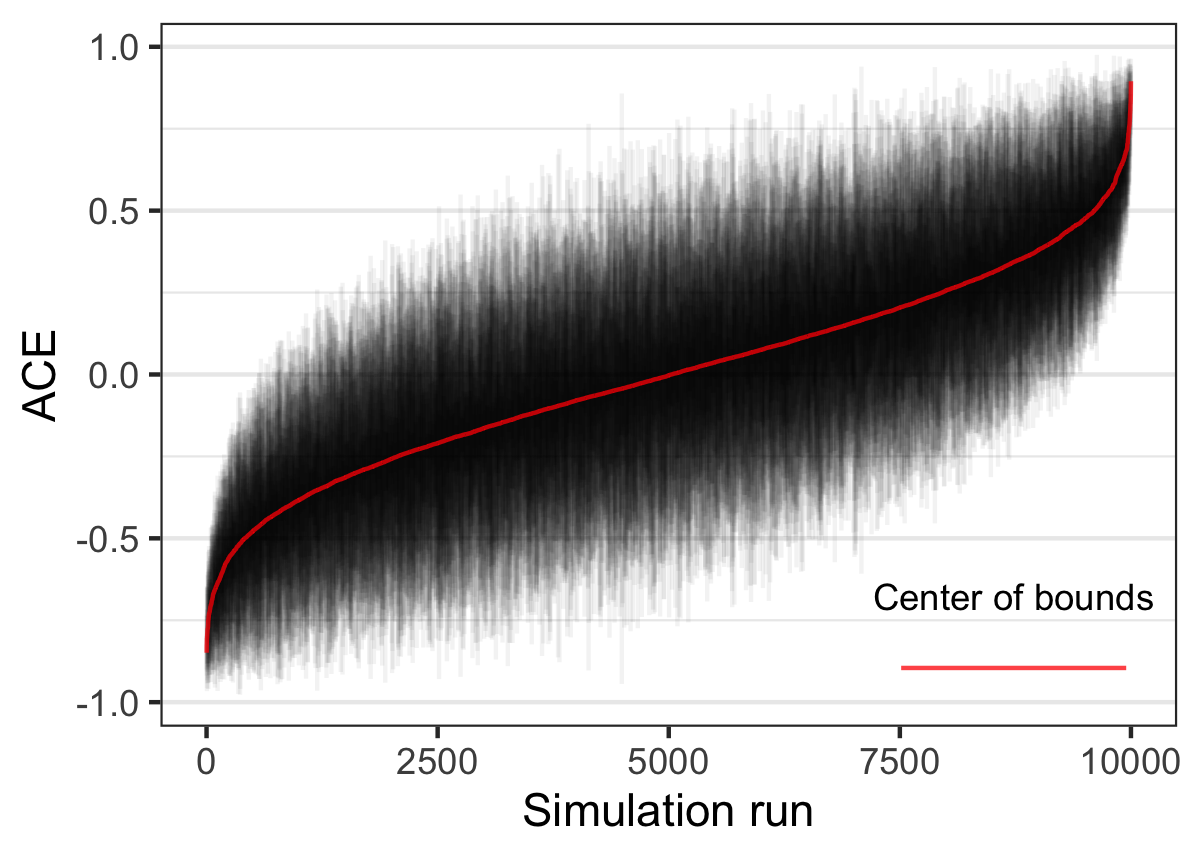
\includegraphics[width=\textwidth]{/Users/ralphtrane/Documents/RPackages_dev/ACEBounds/figures/all_bivariate_bounds.png}
    \caption{Bounds ordered by the center of the bounds.}
    \label{fig:all_biv_bounds}
  \end{subfigure}%
  ~
  \begin{subfigure}[t]{0.5\textwidth}
    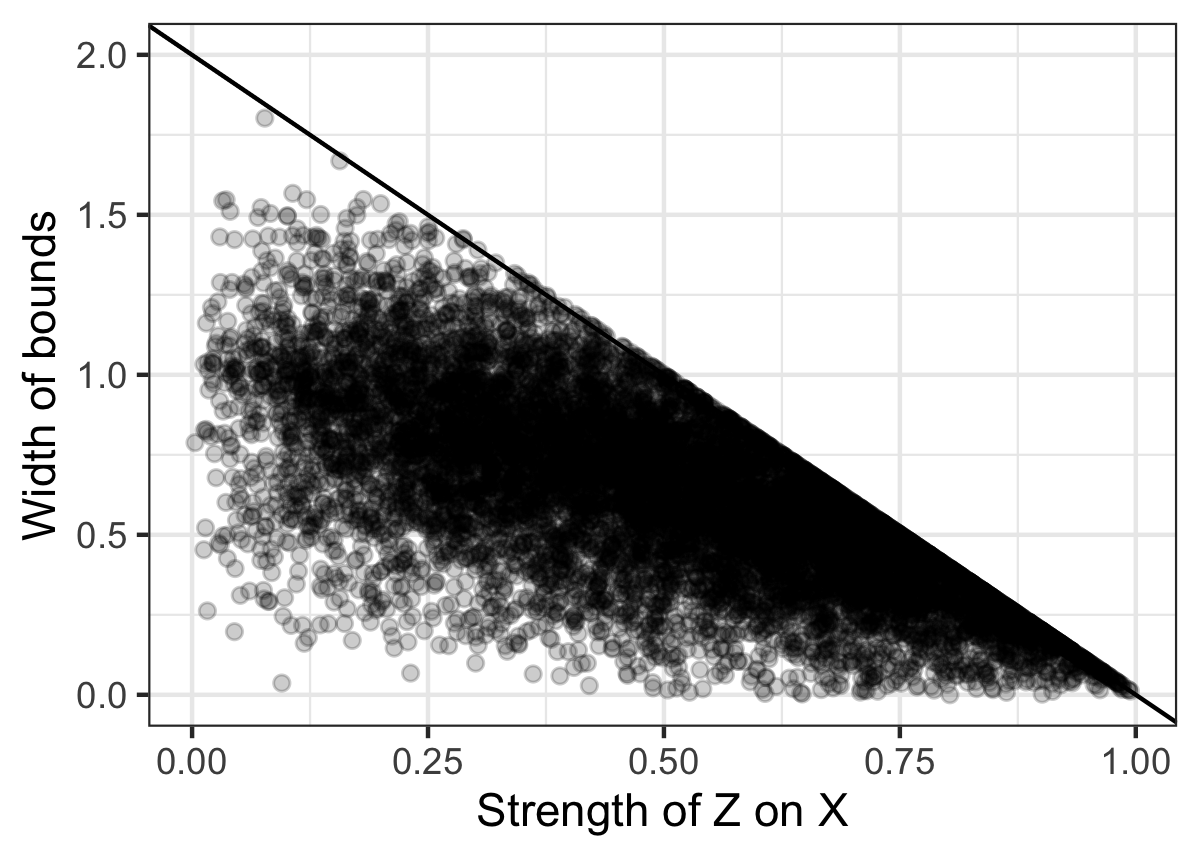
\includegraphics[width=\textwidth]{/Users/ralphtrane/Documents/RPackages_dev/ACEBounds/figures/bivariate_width_vs_strength.png}
    \caption{Black line has intercept 2 and slope -2.}
    \label{fig:biv_width_vs_strength}
  \end{subfigure}
  \caption{10,000 values for bivariate distributions were randomly generated such that no constraints were violated. Of these, 123 resulted in bounds where the lower bound was greater than the upper bounds. These have been removed from these plots.}
  \label{fig:biv_bounds_vs_strength}
\end{figure*}

\textcolor{red}{I think Fig1a may not be as useful as I originally thought...I think Fig a could be perhaps replaced by a version of Fig 1b, but where we actually plot the smoking data example here? Or even find a GWAS in MR-Base where $X$ and $Y$ have strong causal link and there's a very strong genetic determinant (e.g. cholesterol/obesity to heart attack?)} \textcolor{blue}{ RMT: I will try to find such an example.}

Figure \ref{fig:biv_width_vs_strength} shows the widths of the same 9,877 bounds plotted against the strength of the instruments. The black line is the upper bound for the width of the bounds in Theorem \ref{thm:upperBoundWidth}. We see that the width of the bounds frequently exceed \(1\). In particular, Table \ref{tab:prop_of_biv_widths_large} shows that the proportion of the intervals presented on Figure \ref{fig:biv_bounds_vs_strength} with width greater than 1, 0.75, and 0.5, stratified by strength. The table reveals that while is possible to observe bounds with width less than 1, for IVs with strength less than 0.05, \(47\%\) of the bounds lead to widths greater than 1 and about \(46.1\%\) of bounds from IVs with strength between \(0.05\) and \(0.1\) have width greater than 1. Also, only \(62.9\%\) of bounds with strength greater than \(0.5\) have widths less than \(0.5\).

\begin{table}[H]
  \begin{center}
  \caption{Proportion of bounds from distributions where width is greater than $1$, $0.75$, and $0.5$ stratified by strength of the instrument $Z$ on the exposure $X$.}
  \label{tab:prop_of_biv_widths_large}
  
\begin{tabular}{lccc}
\toprule
\multicolumn{1}{c}{ } & \multicolumn{3}{c}{\makecell[c]{Proportion of bounds with\\ width greater than...}} \\
\cmidrule(l{3pt}r{3pt}){2-4}
Strength & 1 & 0.75 & 0.5\\
\midrule
$[0,0.05]$ & $0.4698795$ & $0.7831325$ & $0.8915663$\\
$(0.05,0.1]$ & $0.4611111$ & $0.7222222$ & $0.8944444$\\
$(0.1,0.25]$ & $0.3227061$ & $0.7029549$ & $0.9222395$\\
$(0.25,0.5]$ & $0.1359280$ & $0.4954981$ & $0.8356085$\\
$(0.5,1]$ & $0.0000000$ & $0.0738818$ & $0.3708067$\\
\bottomrule
\end{tabular}


  \end{center}
\end{table}

Overall, in the context of two-sample MR studies with summary statistics, most genetic instruments are weak, which means that the chances that bivariate bounds from MR analyses are informative with width less than 1 are very slim. In particular, a strength requirement of \(\text{ST} > 0.5\) to guarantee a bound with length less than \(1\) is a tall order in many MR studies. \textcolor{red}{Perhaps, convert the difference in probability to roughly what it would correspond to in a logistic model, either as an odds ratio or beta coef? Even tying it to the smoking example by saying that one must find a genetic variant that can change the odds of smoking by a factor of BLANK would be helpful to understand for MR/GWAS practitioners looking at odds ratios/z-stats/p-vals all day.} \textcolor{blue}{ RMT: Can try to do this, but since these are randomly generated, they don't necessarily fit the logistic model setting, i.e. monotonicity might be violated. Thoughts on how to express ST as an OR? Could maybe do a $max OR_{z_1,z_2}$.} Additionally, as our numerical results revealed, a set of bounds with width just below 1 does not provide much more information; a bound of \([-0.1, 0.8]\) for the ATE does not indicate that the average treatment effect is more likely to be positive than a bound of \([-0.7, 0.2]\) for the ATE.

\textcolor{red}{Another good thing that we can perhaps include is a power curve of sorts? That is, given that the effect size to detect is equal to $0.2 = E[P(Y | X=1, U) - P(Y | X = 0, U)]$, what kind of instrument do we need to detect this?}

\textcolor{blue}{Would have to restructure a bit to have more of a simulation rather than a "randomly draw values" setup.}

\hypertarget{bounds-with-multiple-ivs}{%
\subsection{Bounds With Multiple IVs}\label{bounds-with-multiple-ivs}}

Prior section revealed that bounds from two-sample MR studies with summary data require a strong instrument to guarantee meaningful widths. However, it did not address whether the bound can be used improved upon by using multiple instruments. In this section, we consider one approach to aggregate bounds across multiple instruments.

Formally, consider the following logistic model for the outcome when there are multiple instruments

\[
\begin{aligned}
\text{logit}(P(X = 1 | Z_1 = z_1, ..., Z_n = z_n)) &= \beta_0 + \sum_i \beta_i z_i \\
\text{logit}(P(Y = 1 | X = x)) &= \gamma_0 + \gamma_1 x,
\end{aligned}
\]

where \(\text{logit}(a) = \frac{1}{1 + \exp(-a)}\), \(y \in \{0,1\}, x \in \{0,1\}\), \(z_i \in \{0, 1, 2\}\), and \(\beta_i, \gamma_j \in \mathbb{R}\). This particular model is popular in MR \textcolor{red}{I would actually use MR methods/studies to justify this model; I think some of the parametric approaches that I mentioned above use this model}. \textcolor{red}{I should have caught this earlier, but are we simulating unmeasured $U$? Otherwise, the effect of $X$ on $Y$ is not confounded at all and you would be able to estimate without needing IVs}\textcolor{blue}{RMT: I seem to recall we previously discussed this way back when... Right now we do not have any unmeasured confounders, but I'm not sure how to include these when we don't really simulate data, but rather numerically integrate.}

We set \(P(Z_j = 0) = P(Z_j = 2) = 0.25\) and \(P(Z_j = 1) = 0.5\) and \(\gamma_0 = -2, \gamma_1 = 0.2\). We also generate \(\beta_i\) from an i.i.d. uniform distribution with support \(0\) to \(1/n\)\textcolor{red}{Ralph, can we actually draw this from our smoking data's distribution? This way, it doesn't seem like the simulation is highly contrived?}. \textcolor{blue}{RMT: done. One problem with this is that these coefficients are much smaller, which leads to weaker instruments, which makes it nearly impossible to distinguish the intervals from one another.} \textcolor{red}{I just realized that perhaps we should use $p$ instead of $n$ to denote number of IVs since $n$ is typically used for sample size?} \textcolor{blue}{Agree. Will fix}. We then obtain summary-level statistics \(P(Y = 1 | Z_j = z_j)\) and \(P(X = 1 | Z_j = z_j)\) by numerically integration the above model.

Figure \ref{fig:bounds_vs_strength_many_IVs_varying_betas} shows the resulting bounds for the three different values of \(n\) plotted against the strengths of the IVs.

\textcolor{red}{Thinking about this figure more closely and what this section represents, I actually think we need a bit more in-depth discussion about the behavior of multi-IV bounds when IV may be invalid, specifically discussing (1) union bounds and (2) finding a region of $[-1,1]$, say $\mathcal{S}$ where more than 50\% of bounds contain $\mathcal{S}$; the latter idea is inspired by the fact that if majority of the IVs are valid, then all these valid IV bounds will contain the ATE and thus, we only need to find the region of $[-1,1]$ where majority of the IV bounds agree on.}

\begin{figure}[H]
  \center
  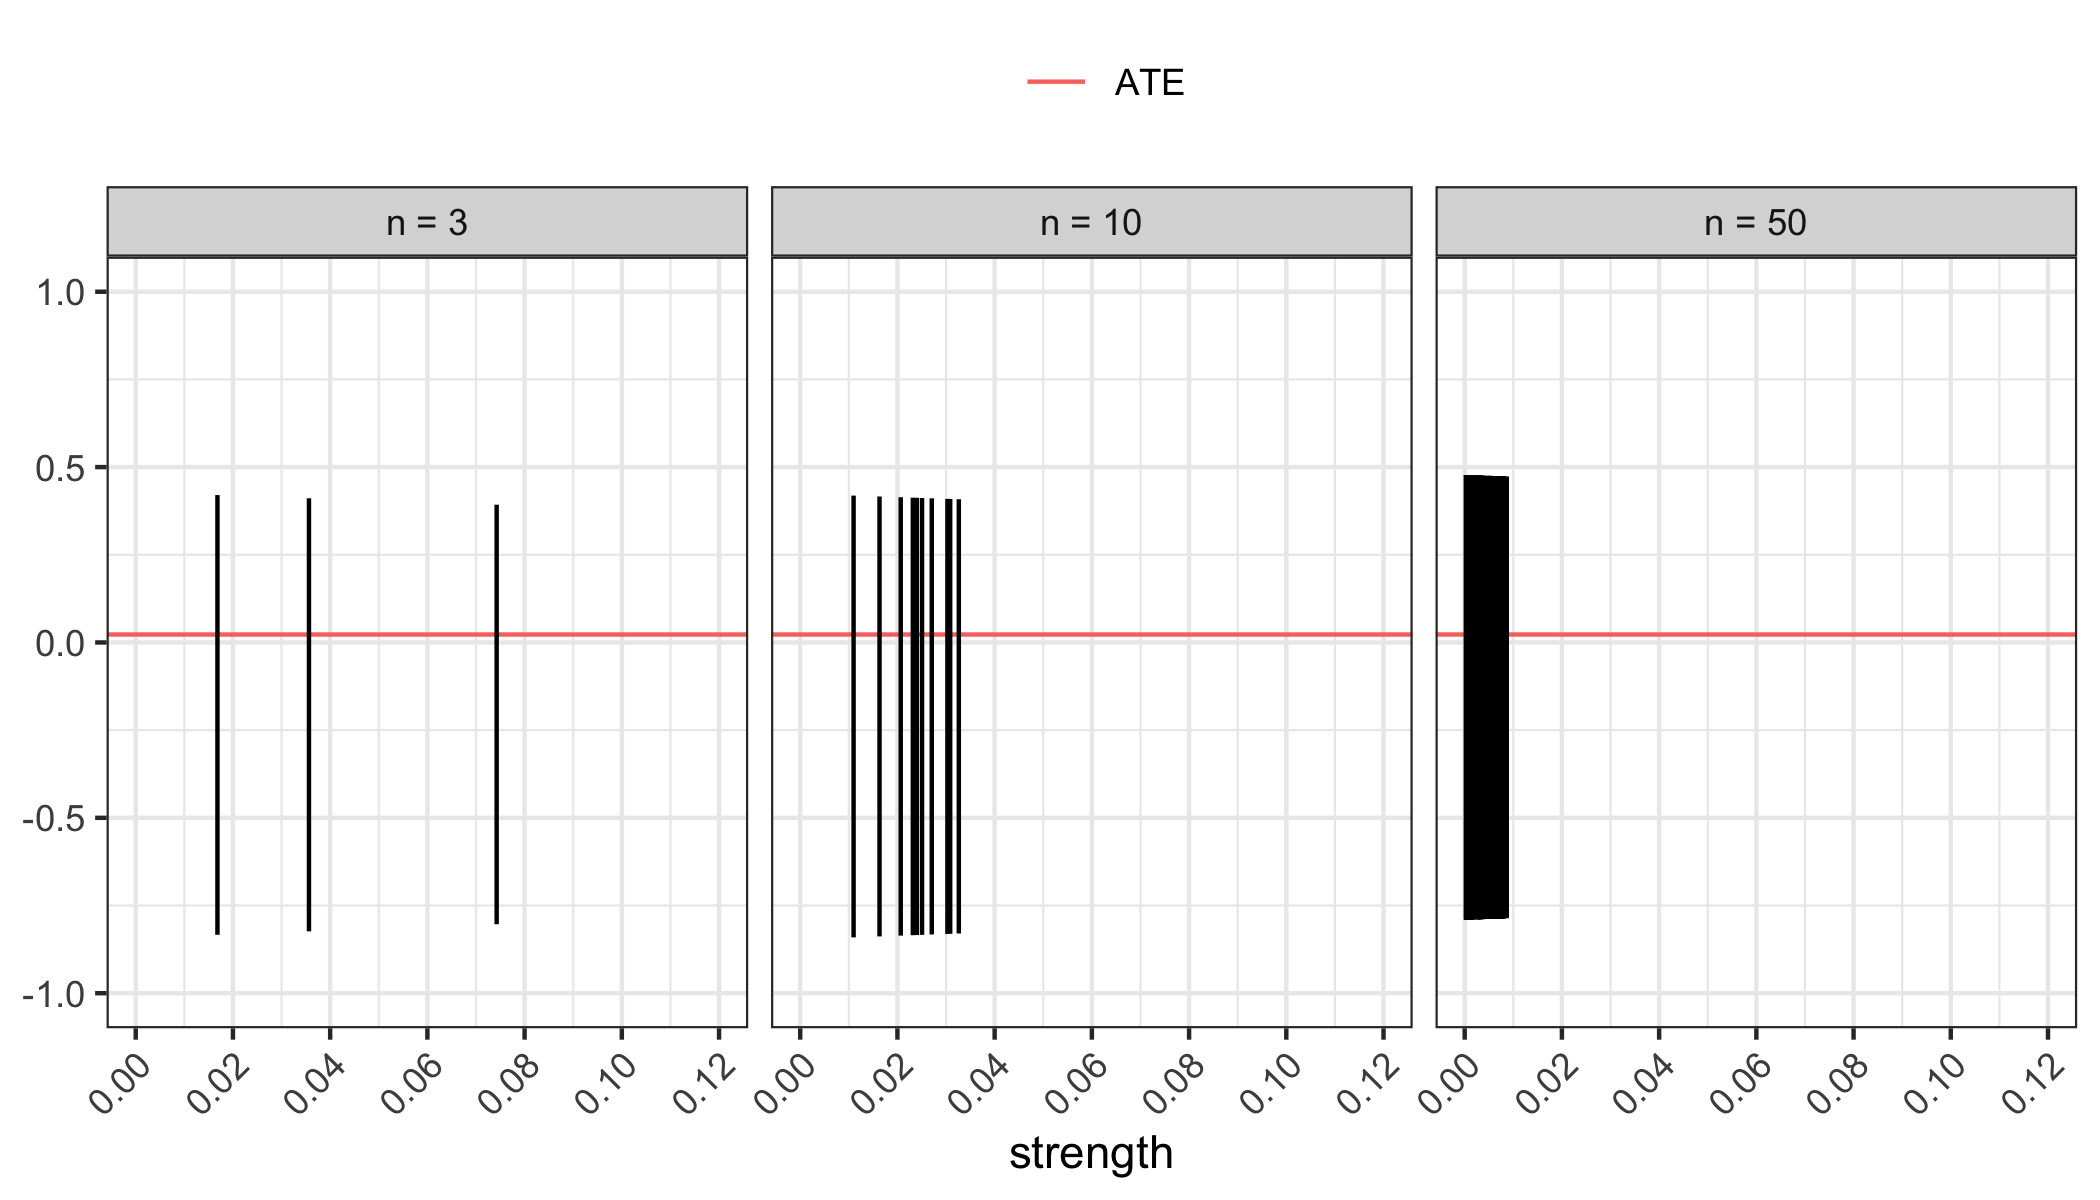
\includegraphics[width = .99\linewidth]{/Users/ralphtrane/Documents/RPackages_dev/ACEBounds/figures/varying_betas_bounds_vs_strength_no_mono.png}
  \caption{Bounds based on probabilities derived from the logistic model. Here, the coefficients are randomly chosen as $\text{Uniform}(0, 1/n)$ for different values of $n$.}
  \label{fig:bounds_vs_strength_many_IVs_varying_betas}
\end{figure}

Our results suggest that if all the instruments are valid, aggregating information from multiple instruments through intersections will not result in more information than simply using a single, strongest individual bound. If, on the other hand, some instruments do not satisfy the IV assumptions and one takes a conservative approach by taking unions of bounds, the resulting bound would be valid in the sense that it will cover the true ATE. But, the union bound would be extremely conservative and ultimately provide even less information about the ATE. While other approaches to aggregation are possible, \textcolor{red}{work on later}

Combining our investigation into the behavior of bounds from Section \ref{bounds-from-bivariate-data}, our general conclusion is that constructing bounds for two-sample MR studies with summary data rely on few assumptions, but are rarely informative. The two primarily reasons for this is that (1) genetic instruments in MR are generally weak, leading to wide bounds and (2) only two-sample data is available to construct bounds. Without having strong instruments in the study, reason (1) is generally difficult, if not impossible, to address with any statistical methodology. Also, unless we change how MR data is collected, going from one-sample to two-sample studies, reason (2) is challenging, but not necessarily impossible, to address. In particular, in the next section, we discuss how to obtain a plausible range of the joint distribution of the outcome and the exposure given the instrument \(P(Y, X | Z)\) given two sample MR data \(P(Y|Z)\) and \(P(X | Z)\) in order to create more informative bounds from two-sample MR studies.

\hypertarget{what-can-you-do-with-summary-level-data-for-bounds-a-quasi-bayesian-path-to-more-information}{%
\section{What can you do with summary-level data for bounds? A Quasi-Bayesian Path to More Information}\label{what-can-you-do-with-summary-level-data-for-bounds-a-quasi-bayesian-path-to-more-information}}

\label{quasi-bayesian}

Our approach to creating more informative bounds from two-sample MR rests on creating a plausible range of the joint distribution of the outcome and the exposure given the instrument \(Z\), \(P(X = x, Y = y | Z = z)\). The plausible range of the joint distribution is informed by quantities available from two-sample MR studies, specifically \(P(X = x | Z = z)\) and \(P(Y = y | Z = z)\), as well as the constraints imposed by the IV assumptions.

Formally, the joint conditional distribution \(P(X = x, Y = y | Z = z)\) is a function of the marginal conditional distributions \(P(X = x | Z = z)\) and \(P(Y = y | Z = z)\) and the conditional covariance of the exposure \(X\) and \(Y\) given \(Z=z\) \(\text{Cov}(X, Y | Z = z)\) for each \(z\)

\begin{equation}
P(X = x, Y = y | Z = z) = P(X = x | Z = z)P(Y = y | Z = z) + (2\cdot I[x = y] - 1)\text{Cov}(X, Y | Z = z). \label{eq:cov-expression}
\end{equation}

Since \(\text{Cov}(X, Y | Z = z)\) is impossible to estimate \textcolor{blue}{from two-sample data}, we instead propose to put a uniform flat prior on this quantity that also results in the joint conditional distribution of \((X,Y|Z)\) being an actual probability distribution and satisfying the verifiable constraints \eqref{eq:constraints} from the IV assumptions. Specifically, by the definition of a proper probability distribution, \(\text{Cov}(X, Y | Z = z)\) must satisfy \textcolor{red}{If you want, I think we can make a lemma out of this?} \textcolor{blue}{RMT: do you think that would be beneficial? I can definitely reword this part as a lemma.}

\[
\begin{aligned}
  \max_z\left\{
      \begin{array}{c}
        -P(X = 1 | Z = z)P(Y = 1 | Z = z) \\
        -P(X = 0 | Z = z)P(Y = 0 | Z = z) \\
        P(X = 1 | Z = z)P(Y = 0 | Z = z) - 1\\
        P(X = 0 | Z = z)P(Y = 1 | Z = z) - 1
      \end{array}
    \right\} & \\
    \le \text{Cov}(X, &Y | Z = z) \le \\
    &\min_z\left\{
      \begin{array}{c}
        1 - P(X = 1 | Z = z)P(Y = 1 | Z = z) \\
        1 - P(X = 0 | Z = z)P(Y = 0 | Z = z) \\
        P(X = 1 | Z = z)P(Y = 0 | Z = z) \\
        P(X = 0 | Z = z)P(Y = 1 | Z = z)
      \end{array}
    \right\}
\end{aligned}
\]

Additionally, by the IV inequality constraints, for any pair of \((z_1, z_2) \in \{0,1,2\} \times \{0,1,2\}\), the values of \(\text{Cov}(X, Y | Z = z_1)\) and \(\text{Cov}(X, Y | Z = z_2)\) must satisfy

\[
\begin{aligned}
  \max\left\{
      \begin{array}{c}
        -P(X = 0 | Z = z_1)P(Y = 0 | Z = z_1) - P(X = 0 | Z = z_2)P(Y = 1 | Z = z_2) \\
        P(X = 1 | Z = z_1)P(Y = 0 | Z = z_1) + P(X = 1 | Z = z_2)P(Y = 1 | Z = z_2) -1 \\
        P(X = 0 | Z = z_2)P(Y = 0 | Z = z_2) + P(X = 0 | Z = z_1)P(Y = 1 | Z = z_1) - 1 \\
        -P(X = 1 | Z = z_2)P(Y = 0 | Z = z_2) - P(X = 1 | Z = z_1)P(Y = 1 | Z = z_1)
      \end{array}
    \right\} \qquad \qquad & \\ \\
    \le \text{Cov}(X,Y | Z = z_1) - \text{Cov}(X,Y | Z = z_2) \le \qquad \qquad \qquad \qquad  \qquad& \\ \\
    \min\left\{
      \begin{array}{c}
        1 -P(X = 0 | Z = z_1)P(Y = 0 | Z = z_1) - P(X = 0 | Z = z_2)P(Y = 1 | Z = z_2) \\
        P(X = 1 | Z = z_1)P(Y = 0 | Z = z_1) + P(X = 1 | Z = z_2)P(Y = 1 | Z = z_2) \\
        P(X = 0 | Z = z_2)P(Y = 0 | Z = z_2) + P(X = 0 | Z = z_1)P(Y = 1 | Z = z_1) \\
        1 - P(X = 1 | Z = z_2)P(Y = 0 | Z = z_2) - P(X = 1 | Z = z_1)P(Y = 1 | Z = z_1)
      \end{array}
    \right\} &
\end{aligned}
\]

Then, we sequentially sample values of \(\text{Cov}(X, Y | Z = 0), \text{Cov}(X, Y | Z = 1), \text{Cov}(X, Y | Z = 2)\), such that the above inequalities plus the existing constraints in \eqref{eq:constraints} are satisfied. Then, among samples of \(\text{Cov}(X, Y | Z = 0), \text{Cov}(X, Y | Z = 1), \text{Cov}(X, Y | Z = 2)\) that satisfy the constraints, we calculate the joint distribution of \(P(X = x, Y = y | Z = z)\) using \eqref{eq:cov-expression}. Ultimately, we have a plausible set of the joint distribution \(P(X = x, Y = y | Z = z)\).

For each plausible set of the joint distribution of \(P(X = x, Y = y | Z = z)\), we use the usual IV bounds by \citet{balke_bounds_1997} and \citet{richardson_ace_2014} from one-sample IV studies to obtain a bound for the ATE. If a large number of these bounds do not cover zero, then there is some evidence to suggest of a causal effect of the exposure and only reason we are not able to detect this effect is due to the limitations of the two-sample design. However, if the majority of these IV bounds do cover zero, there is less evidence to suggest a causal exposure effect and/or that utilizing bounds to obtain some information about the ATE may be a hopeless exercise. In short, we are trying answer ``had we observed one-sample data that satisfies the constraints of the two-sample data we currently have, could we have detected the presence of an exposure effect?''

The approach above can be thought of as using a quasi-empirical bayesian framework for partially identified sets. Specifically, our procedure generates a posterior distribution of IV bounds given the marginalized probabilities from two-sample data (i.e.~the likelihood) and a uniform, flat prior on the unknown quantities \(\text{Cov}(X, Y | Z = z)\). The constraints that we impose on \(\text{Cov}(X, Y | Z = z)\) are almost empirically Bayesian in nature as they are informed by data from two-sample MR.

\hypertarget{single-instrument}{%
\subsection{Single Instrument}\label{single-instrument}}

We illustrate the potential utility of the proposed method from the previous section by considering nine hypothetical MR studies, each using one instrument; see Section \ref{multiple-iv-case} for the case with multiple instruments. Table \ref{tab:subset_plot_summaries_b} presents nine different sets of values of the marginal distributions \(P(Y|Z)\) and \(P(X | Z)\) from nine hypothetical two-sample MR studies \textcolor{red}{Do you think we can find an empirical example to support some of these nine from MR-Base? I'm thinking about using popular exposures in the MR field (like CRP, cholesterol, or vitamin D?)} \textcolor{blue}{ RMT: I will take a look.}.

\begin{table}[H]
  \center
  \caption{Values of $P(X = 1 | Z = z)$ and $P(Y = 1 | Z = z)$ used to illustrate our quasi-bayesian approach. These are presented with $\{P(X = 1 | Z = 0), P(X = 1 | Z = 1), P(X = 1 | Z = 2)\}$ on the first row, and $\{P(Y = 1 | Z = 0), P(Y = 1 | Z = 1), P(Y = 1 | Z = 2)\}$ on the second row.}
  \label{tab:subset_plot_summaries_b}
  
\begin{tabular}{llll}
\toprule
  & Column 1 & Column 2 & Column 3\\
\midrule
Row a & \makecell[l]{\{0.125, 0.399, 0.080\}\\\{0.699, 0.840, 0.742\}} & \makecell[c]{\{0.244, 0.275, 0.185\}\\\{0.238, 0.089, 0.146\}} & \makecell[r]{\{0.603, 0.469, 0.310\}\\\{0.638, 0.346, 0.719\}}\\
Row b & \makecell[l]{\{0.886, 0.968, 0.874\}\\\{0.805, 0.822, 0.951\}} & \makecell[c]{\{0.139, 0.441, 0.334\}\\\{0.179, 0.359, 0.559\}} & \makecell[r]{\{0.901, 0.909, 0.935\}\\\{0.821, 0.810, 0.905\}}\\
Row c & \makecell[l]{\{0.175, 0.079, 0.365\}\\\{0.599, 0.358, 0.087\}} & \makecell[c]{\{0.493, 0.911, 0.085\}\\\{0.360, 0.480, 0.441\}} & \makecell[r]{\{0.434, 0.045, 0.733\}\\\{0.747, 0.370, 0.169\}}\\
\bottomrule
\end{tabular}


\end{table}

\begin{figure}[H]
  \center
  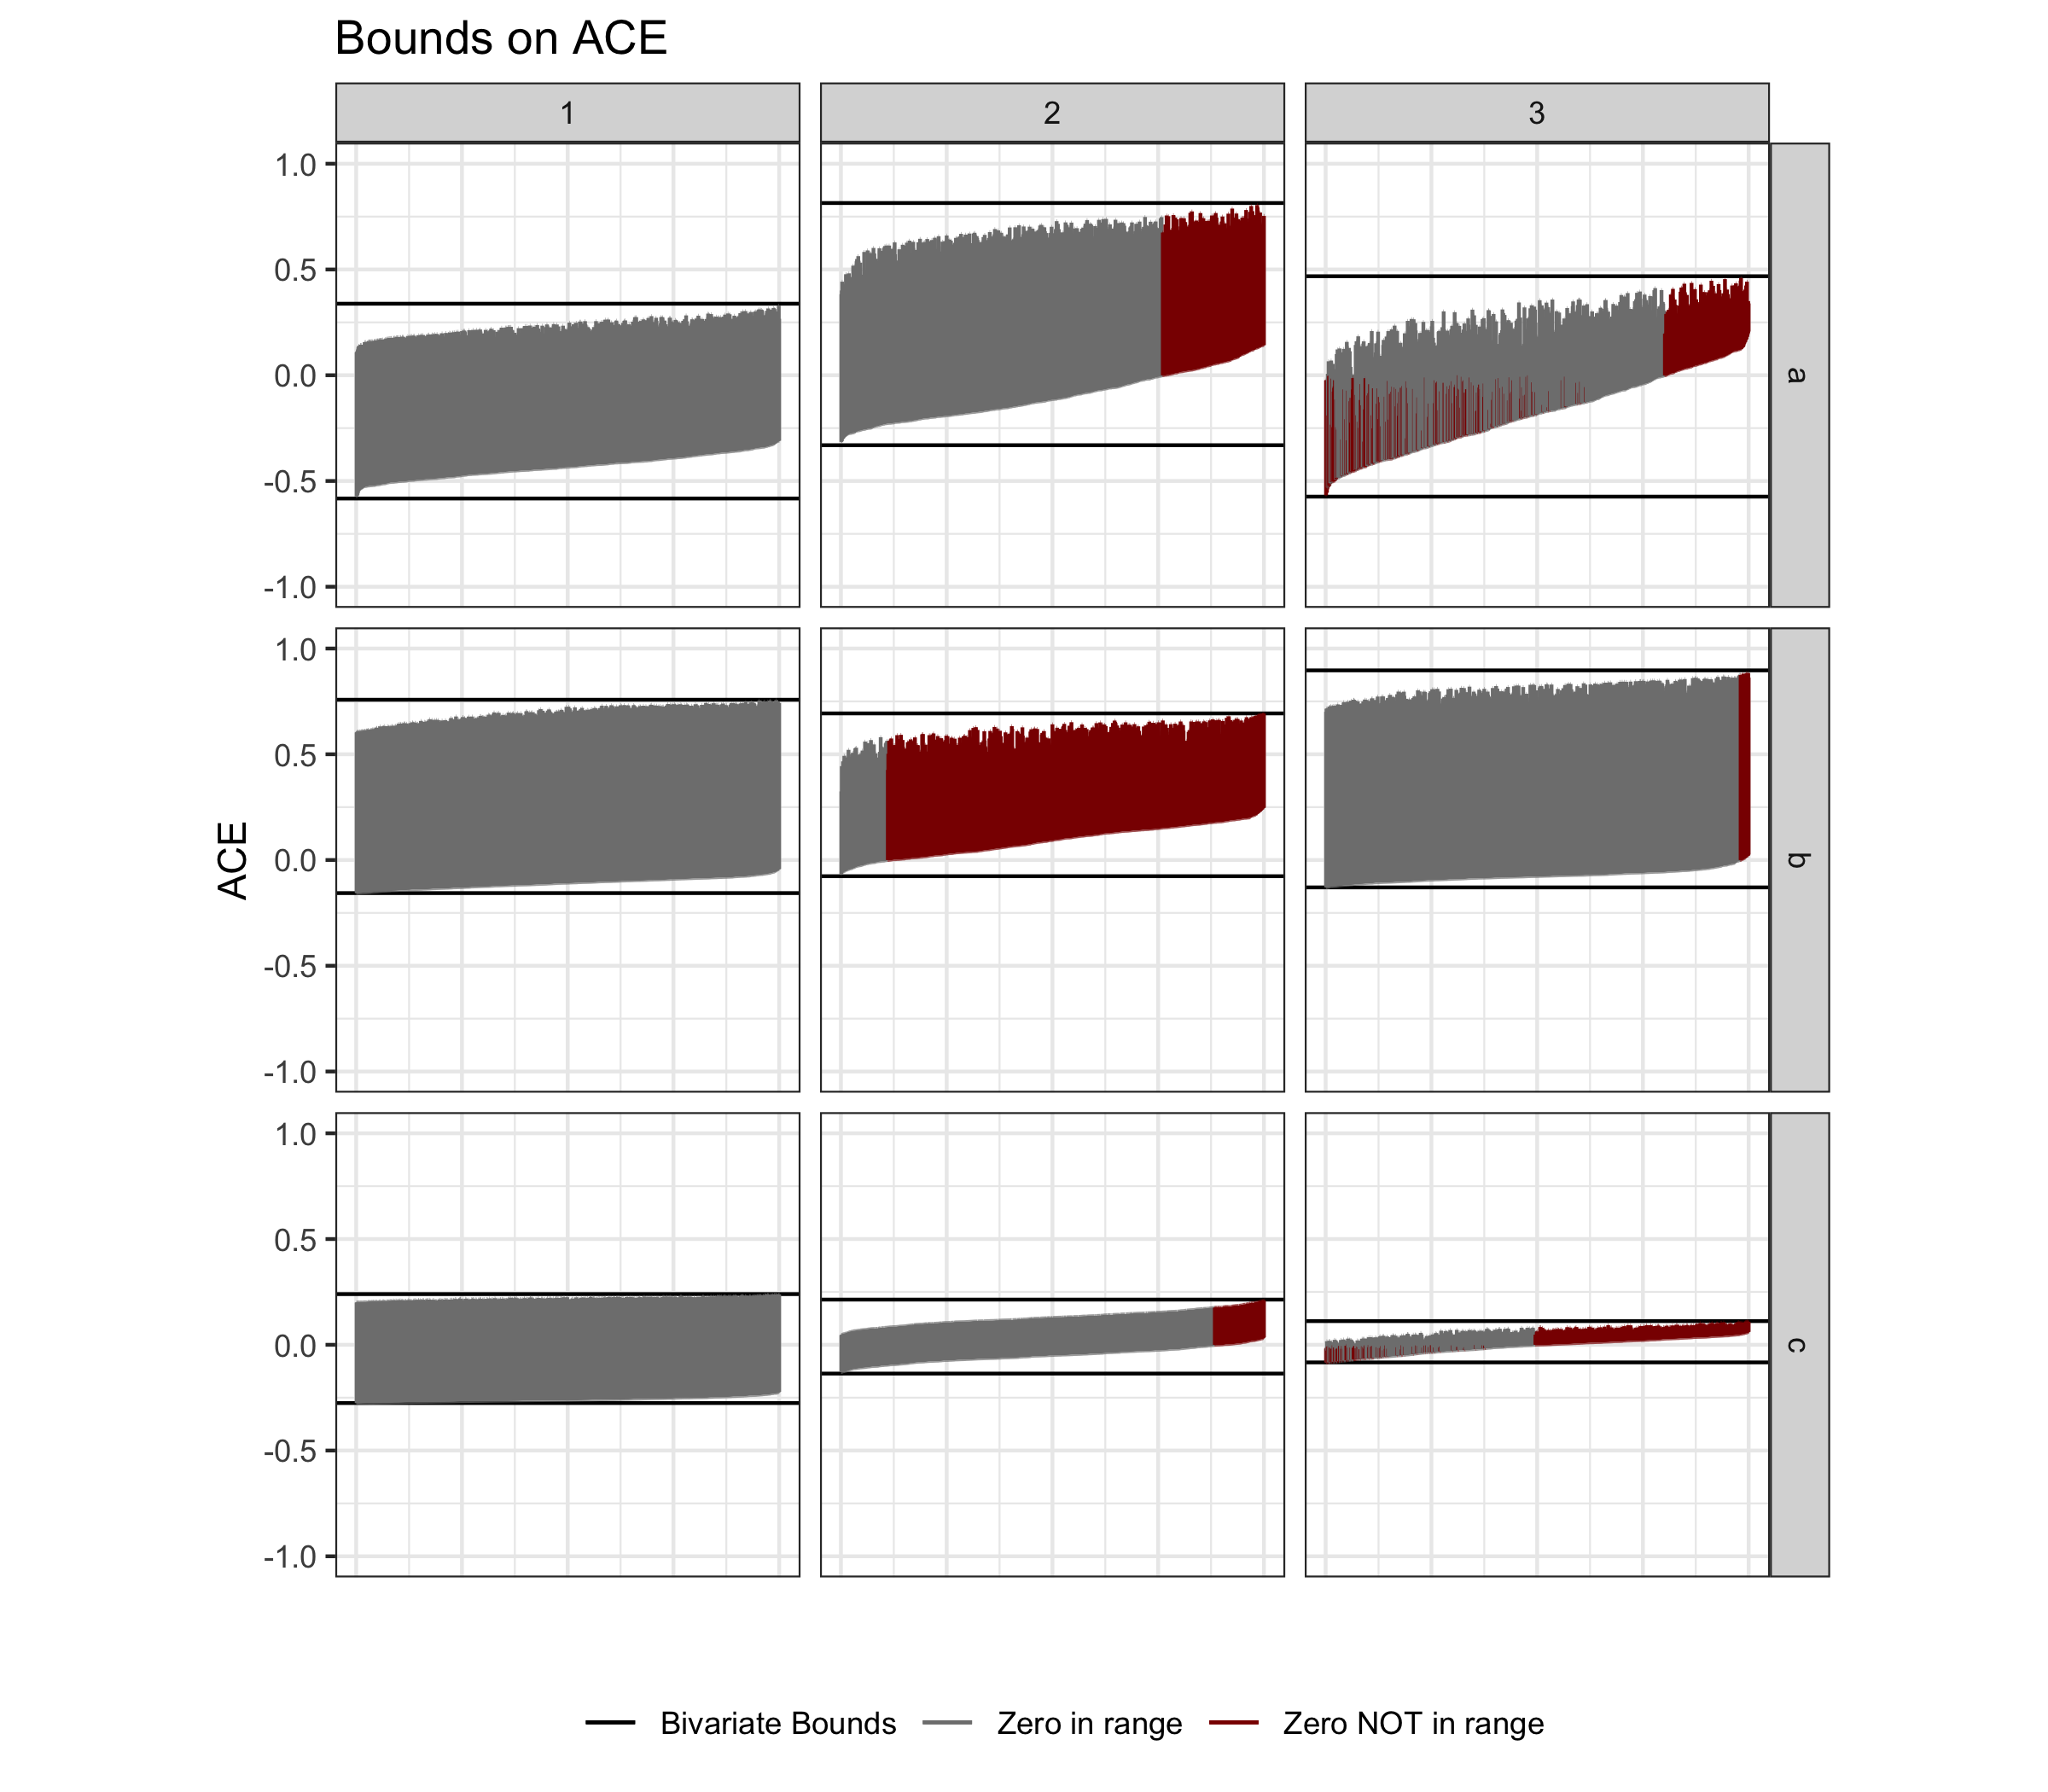
\includegraphics[width=\linewidth]{/Users/ralphtrane/Documents/RPackages_dev/ACEBounds/figures/trivariate_bounds_subset_plot.png}
  \caption{One-sample and two-sample bounds. Even similar bivariate distributions can result in very different insights.}
  \label{fig:trivariate_bounds}
\end{figure}

Figure \ref{fig:trivariate_bounds} shows the resulting bounds only using two-sample data and the set of plausible one-sample IV bounds from our procedure. Row a shows three scenarios where the two-sample bounds are all more or less centered around zero with similar widths. However, the conclusions are rather different. Column 1 shows no one-sample bounds would allow us to determine the presence of a non-zero causal effect. Column 2 indicates that about 24\% of the one-sample IV bounds does not contain \(0\) while for column 3 that number is approximately 36.8\%. However, while the direction of the effect is always the same for column 2 (positive), it varies for column 3.

Row b illustrates three scenarios where the two-sample bounds are centered well above zero and have large widths. Here, we see one case where we have no hope of determining direction from the one-sample bounds (column 1), one case where we are most likely to be able to determine the direction of the ATE to be positive from the one-sample bounds (column 2), and one case where we are rather unlikely to be able to determine the direction of the ATE from the one-sample bounds (column 3).

Row c is similar to row a in that all the two-sample bounds are centered around 0, but the width of the two-sample bounds are narrow. The three columns indicate similar conclusions as seen in row a. This shows that even with rather narrow two-sample bounds centered around 0, the one-sample bounds may still be have to reveal some information about presence as well as the direction of the exposure effect.

Some caution should be exercised when interpreting the proportion of one-sample bounds not containing \(0\). A scenario like the one resulting in the bounds presented in row b, column 2 only provides information about the one-sample bounds, but only if our flat prior on \(\text{Cov}(X,Y|Z)\) is correct. Under this prior, it tells us that it is much more likely that the ATE is positive. It does not, however, rule out a negative value of the ATE, but it does rule out the possibility of one-sample bounds being able to determine direction \emph{if the ATE is in fact negative}. More generally, the conclusion we can reach from our approach hinges on the instrument satisfying the IV assumptions presented in Section \ref{iv-assumptions-and-two-sample-mr}.

\hypertarget{multiple-instruments}{%
\subsection{Multiple Instruments}\label{multiple-instruments}}

Although the bivariate bounds often do not provide much information themselves, as we saw in the previous section, the little information available can sometimes provide some insights. The approach presented draws on the fact that trivariate bounds are guaranteed to be much narrower than bivariate bounds. It remains to be seen if utilizing such an approach while aggregating information from multiple IVs through intersections of bounds can be useful.

The simplest extension to the multiple IV scenario, is to simply repeat the sampling procedure presented in Section \ref{sampling-procedure} for each proposed instrument before creating the combined bounds by taking the intersection of the pairwise bounds. This builds on one main assumption in that the two sampling procedures are done independently, and so implicitly assume that the covariances of \(X\) and \(Y\) given \(Z_1\) are independent of the covariances of \(X\) and \(Y\) given \(Z_2\).

Specifically, say we get bounds \((LB_{1i},UB_{1i}),i = 1,2,...,m\) by sampling m trivariate distributions based on the information we have on \((X,Z_1)\) and \((Y,Z_1)\), and bounds \((LB_{2i}, UB_{2i}),i = 1,2,...,m\) by sampling \(m\) trivariate distributions based on the information we have on \((X,Z_2)\) and \((Y,Z_2)\). We then create the intersection bounds as \(\left(\max_{z \in {1,2}} LB_{zi}, \min_{z \in {1,2}} UB_{zi}\right), i = 1, 2, ..., m\). This, under the assumption that \(\text{Cov}(X, Y | Z_1 = z)\) and \(\text{Cov}(X, Y | Z_2 = z)\) are independent of each other, gives us a sample from the posterior distribution of intersection bounds. We can use this to assess the potential usefulness of aggregating information from two sets of trivariate data, \((X, Y, Z_1)\) and \((X, Y, Z_2)\), using intersection bounds.

We will illustrate this approach in the next section using data obtained from MRBase.

\hypertarget{data-analysis}{%
\section{Data Analysis}\label{data-analysis}}

We consider two example analyses to demonstrate our findings above. Specifically, we aim to study the effect of smoking on lung cancer and depression through an MR analysis. The effect of smoking on lung cancer is well-known to be strong and causal and serves as a positive control to demonstrate the usefulness of the MR analysis via bounds. The effect of smoking on depression has also been studied in other works \citep{wootton_evidence_2019}\textcolor{red}{cite from other MR paper as well as citations within that MR paper}. In both cases, we will explore the non-parametric bounds obtained from two-sample designs and what conclusions are attainable based on our approach.

The data to study both effects was obtained from the UK Biobank data curated at the IEU GWAS database, which is available in R through the \texttt{TwoSampleMR} package \citep{mrbase}. Specifically, data on smoking was obtained from data entry with ID ukb-d-20116\_0, data on depression from entry with ID ukb-d-20544\_11, and data on lung cancer from entry with ID ukb-d-40001\_C349. We followed the defaults of the package where linkage disequilibrium based clumping (\(r^2 \ge 0.001\) within a \(10,000\) kb window using \(p < 5 \times 10^{-8}\) as the level of significance) were performed such that only independent instruments with significant associations are returned. The data was harmonized to make sure that the effects of the SNPs on exposure and outcome were measured with the same allele as reference. Afterwards, we obtain the estimated coefficients from previous GWAS experiments corresponding to the effects of the SNPs on the exposure, and the outcome from a logistic model. Since estimates of the intercept are included in these reported results, but marginal proportions of the outcome, exposure, and allele frequencies are known, we find the intercepts by solving \(P(X = 1) = \sum_{z = 0}^2\text{logit}(\beta_0 + \hat{\beta_1}\cdot z)\cdot P(Z = z)\) and \(P(Y = 1) = \sum_{z = 0}^2\text{logit}(\gamma_0 + \hat{\gamma_1}\cdot z)\cdot P(Z_j = z)\) for \(\beta_0\) and \(\gamma_0\), respectively. Overall, the \texttt{TwoSampleMR} package along with our estimates of the intercept allowed us to calculate \(P(Y = 1 | Z_j = z)\) and \(P(X = 1 | Z_j = z)\) for every \(j\) and \(z=0,1,2\); see {[}link to vignette showing analysis on pkgdown page{]} for the code.

\textcolor{red}{We should stress test this intercept finding (and ultimately, recovering $P(Y|Z)$ and $P(X|Z)$) procedure? For example, I know the FTO-genetic marker is very strongly associated with obesity and hopefully,  $P(X|Z=z) - P(X | Z= z')$ is large? Or, we can also simulate to verify this procedure...}

\textcolor{blue}{RMT: Found a study in mrbase with obesity as outcome. Strongest IVs $\approx 0.065$. Is that large? As for other stress tests, simulations is probably the way to go. Will implement in the coming days.}

\hypertarget{smoking-effect-on-depression}{%
\subsection{Smoking effect on depression}\label{smoking-effect-on-depression}}

Previous reports suggested that smoking increases the risk of depression, with the most recent estimate suggesting the odds ratio to be 1.99 with a 95\% confidence interval of {[}1.71, 2.32{]} \citep{wootton_evidence_2019} based on a non-IV approach. Our MR analysis uses 84 genetic variants as instruments and Figure \ref{fig:strength_histogram} shows a histogram of their strength. We see here that the strength of the strongest instrument is less than 0.01, which is much smaller than the 0.5 needed to guarantee narrow bounds. More information on the instruments and summary statistics can be found in Appendix \ref{more-details-data-application-appendix}.

\begin{figure}[H]
  \center
  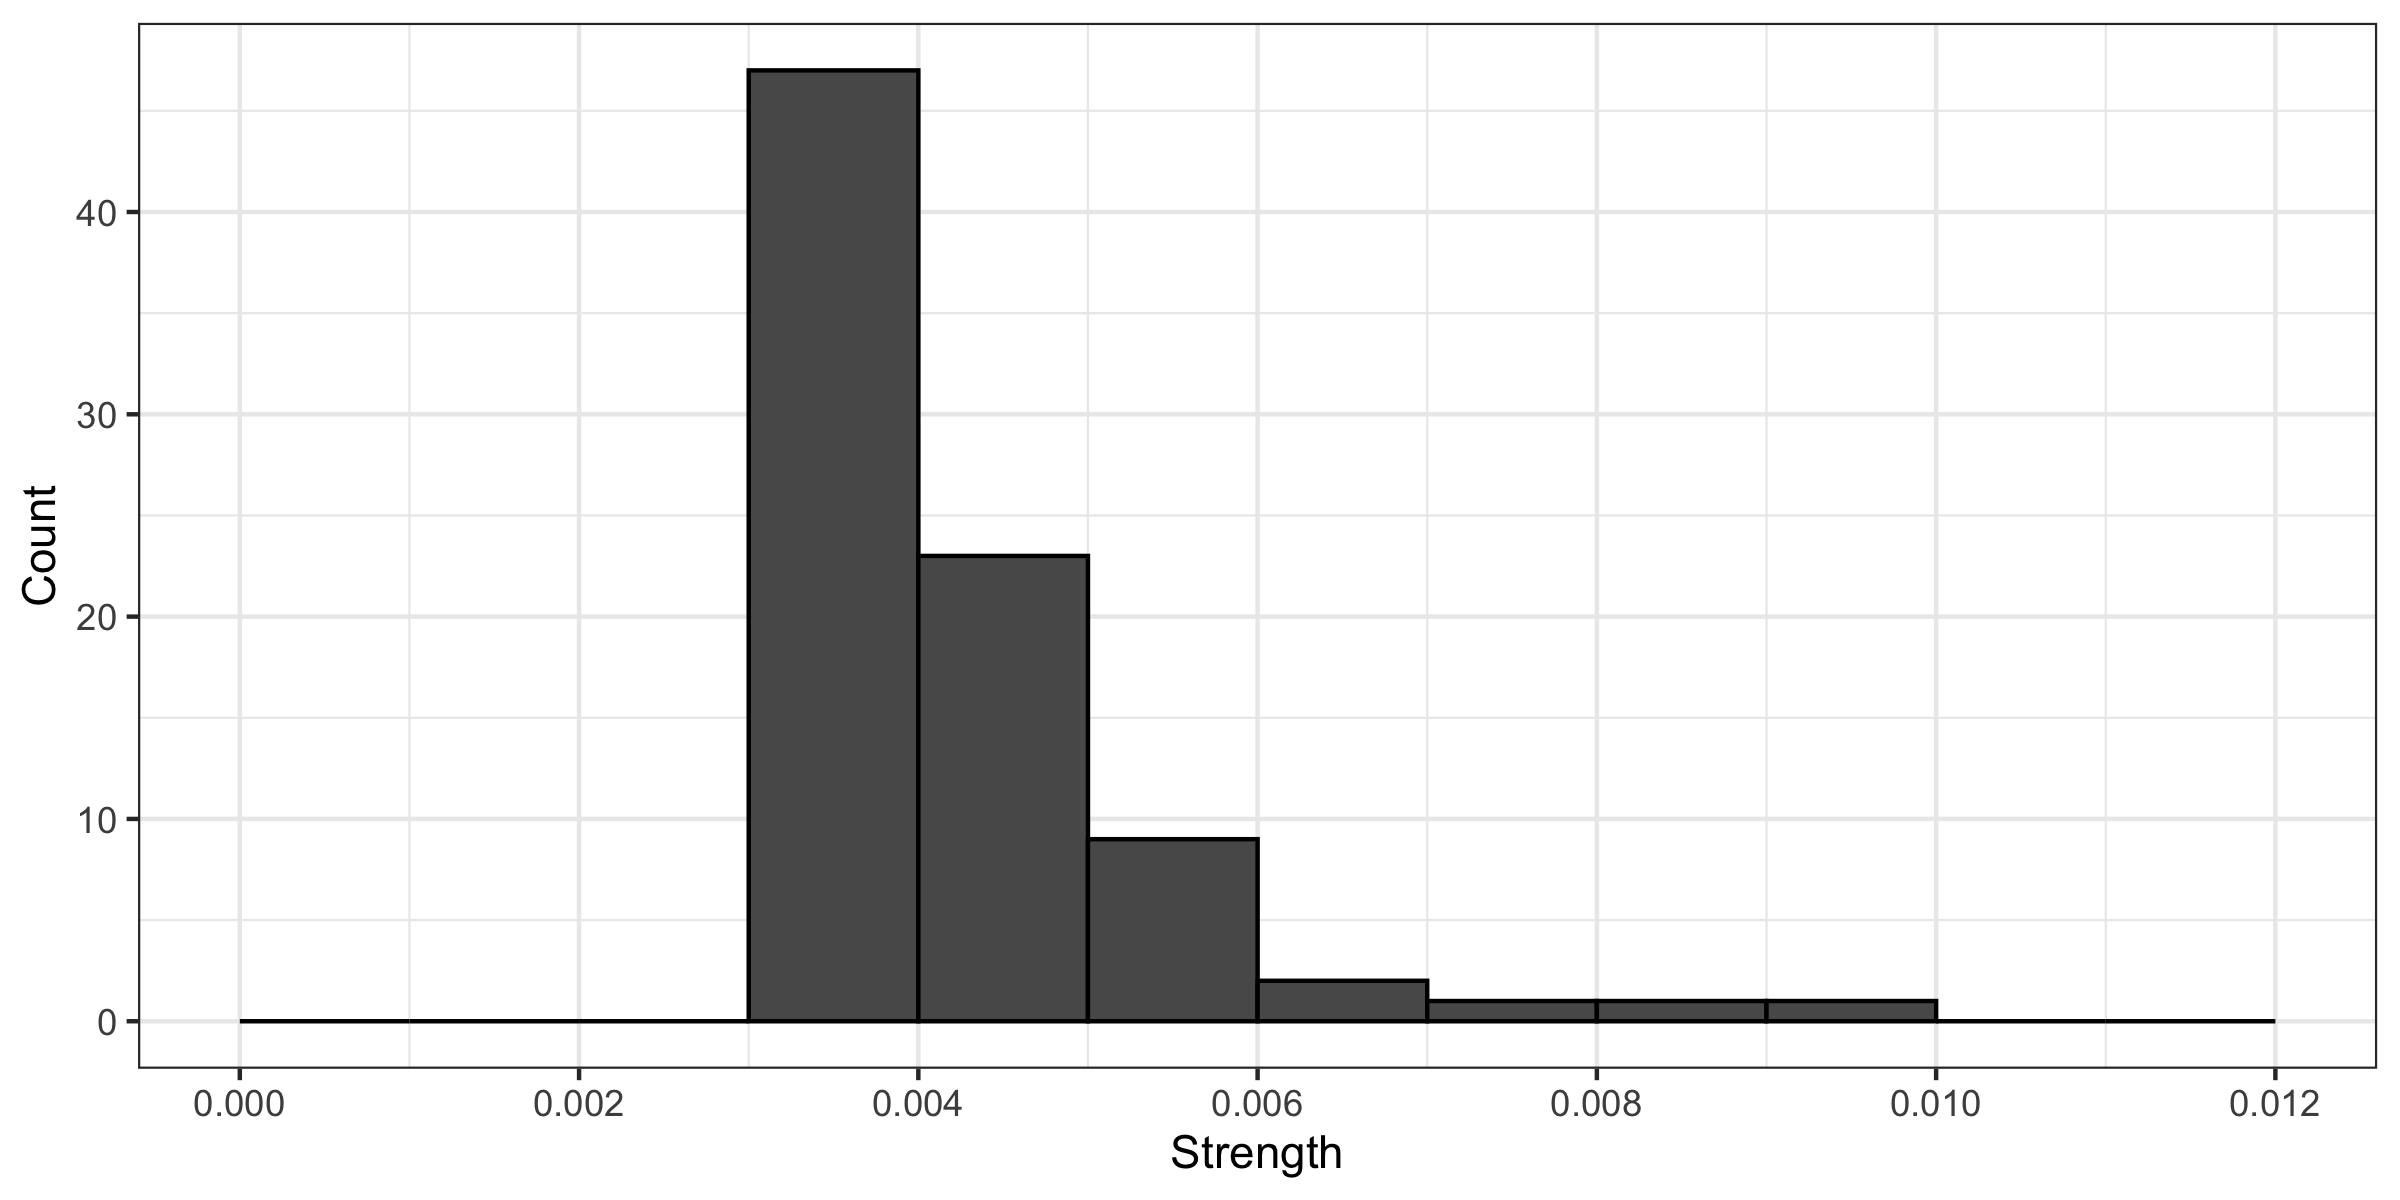
\includegraphics[width = 0.99\linewidth]{/Users/ralphtrane/Documents/RPackages_dev/ACEBounds/figures/example_analyses/strength_histogram.png}
  \caption{Histogram of strengths of IVs on the exposure. Here, SNPs are IVs, and smoking status (ever/never) is exposure. We see that all IVs are very weak, with the largest value just below 0.01.}
  \label{fig:strength_histogram}
\end{figure}

From the 84 instruments, we obtain 84 sets of two-sample bounds and they are shown in Figure \ref{fig:smoking_on_depression_ind_bounds} \textcolor{red}{Can we transpose this graph so that as we go down the page, we have snps and the x-axis is the bounds?}. From this figure, it is immediately clear that all the intervals are practically identical and none of them provide any information about the presence of an effect. Also, aggregating across 84 bounds, either by intersection or union, will not reveal any useful insights about the exposure effect. This is not surprising given that all instruments are very weak and our analysis in Section 3.1 showed that weak instruments in two-sample settings tend to lead to large bounds.

\begin{figure}[H]
  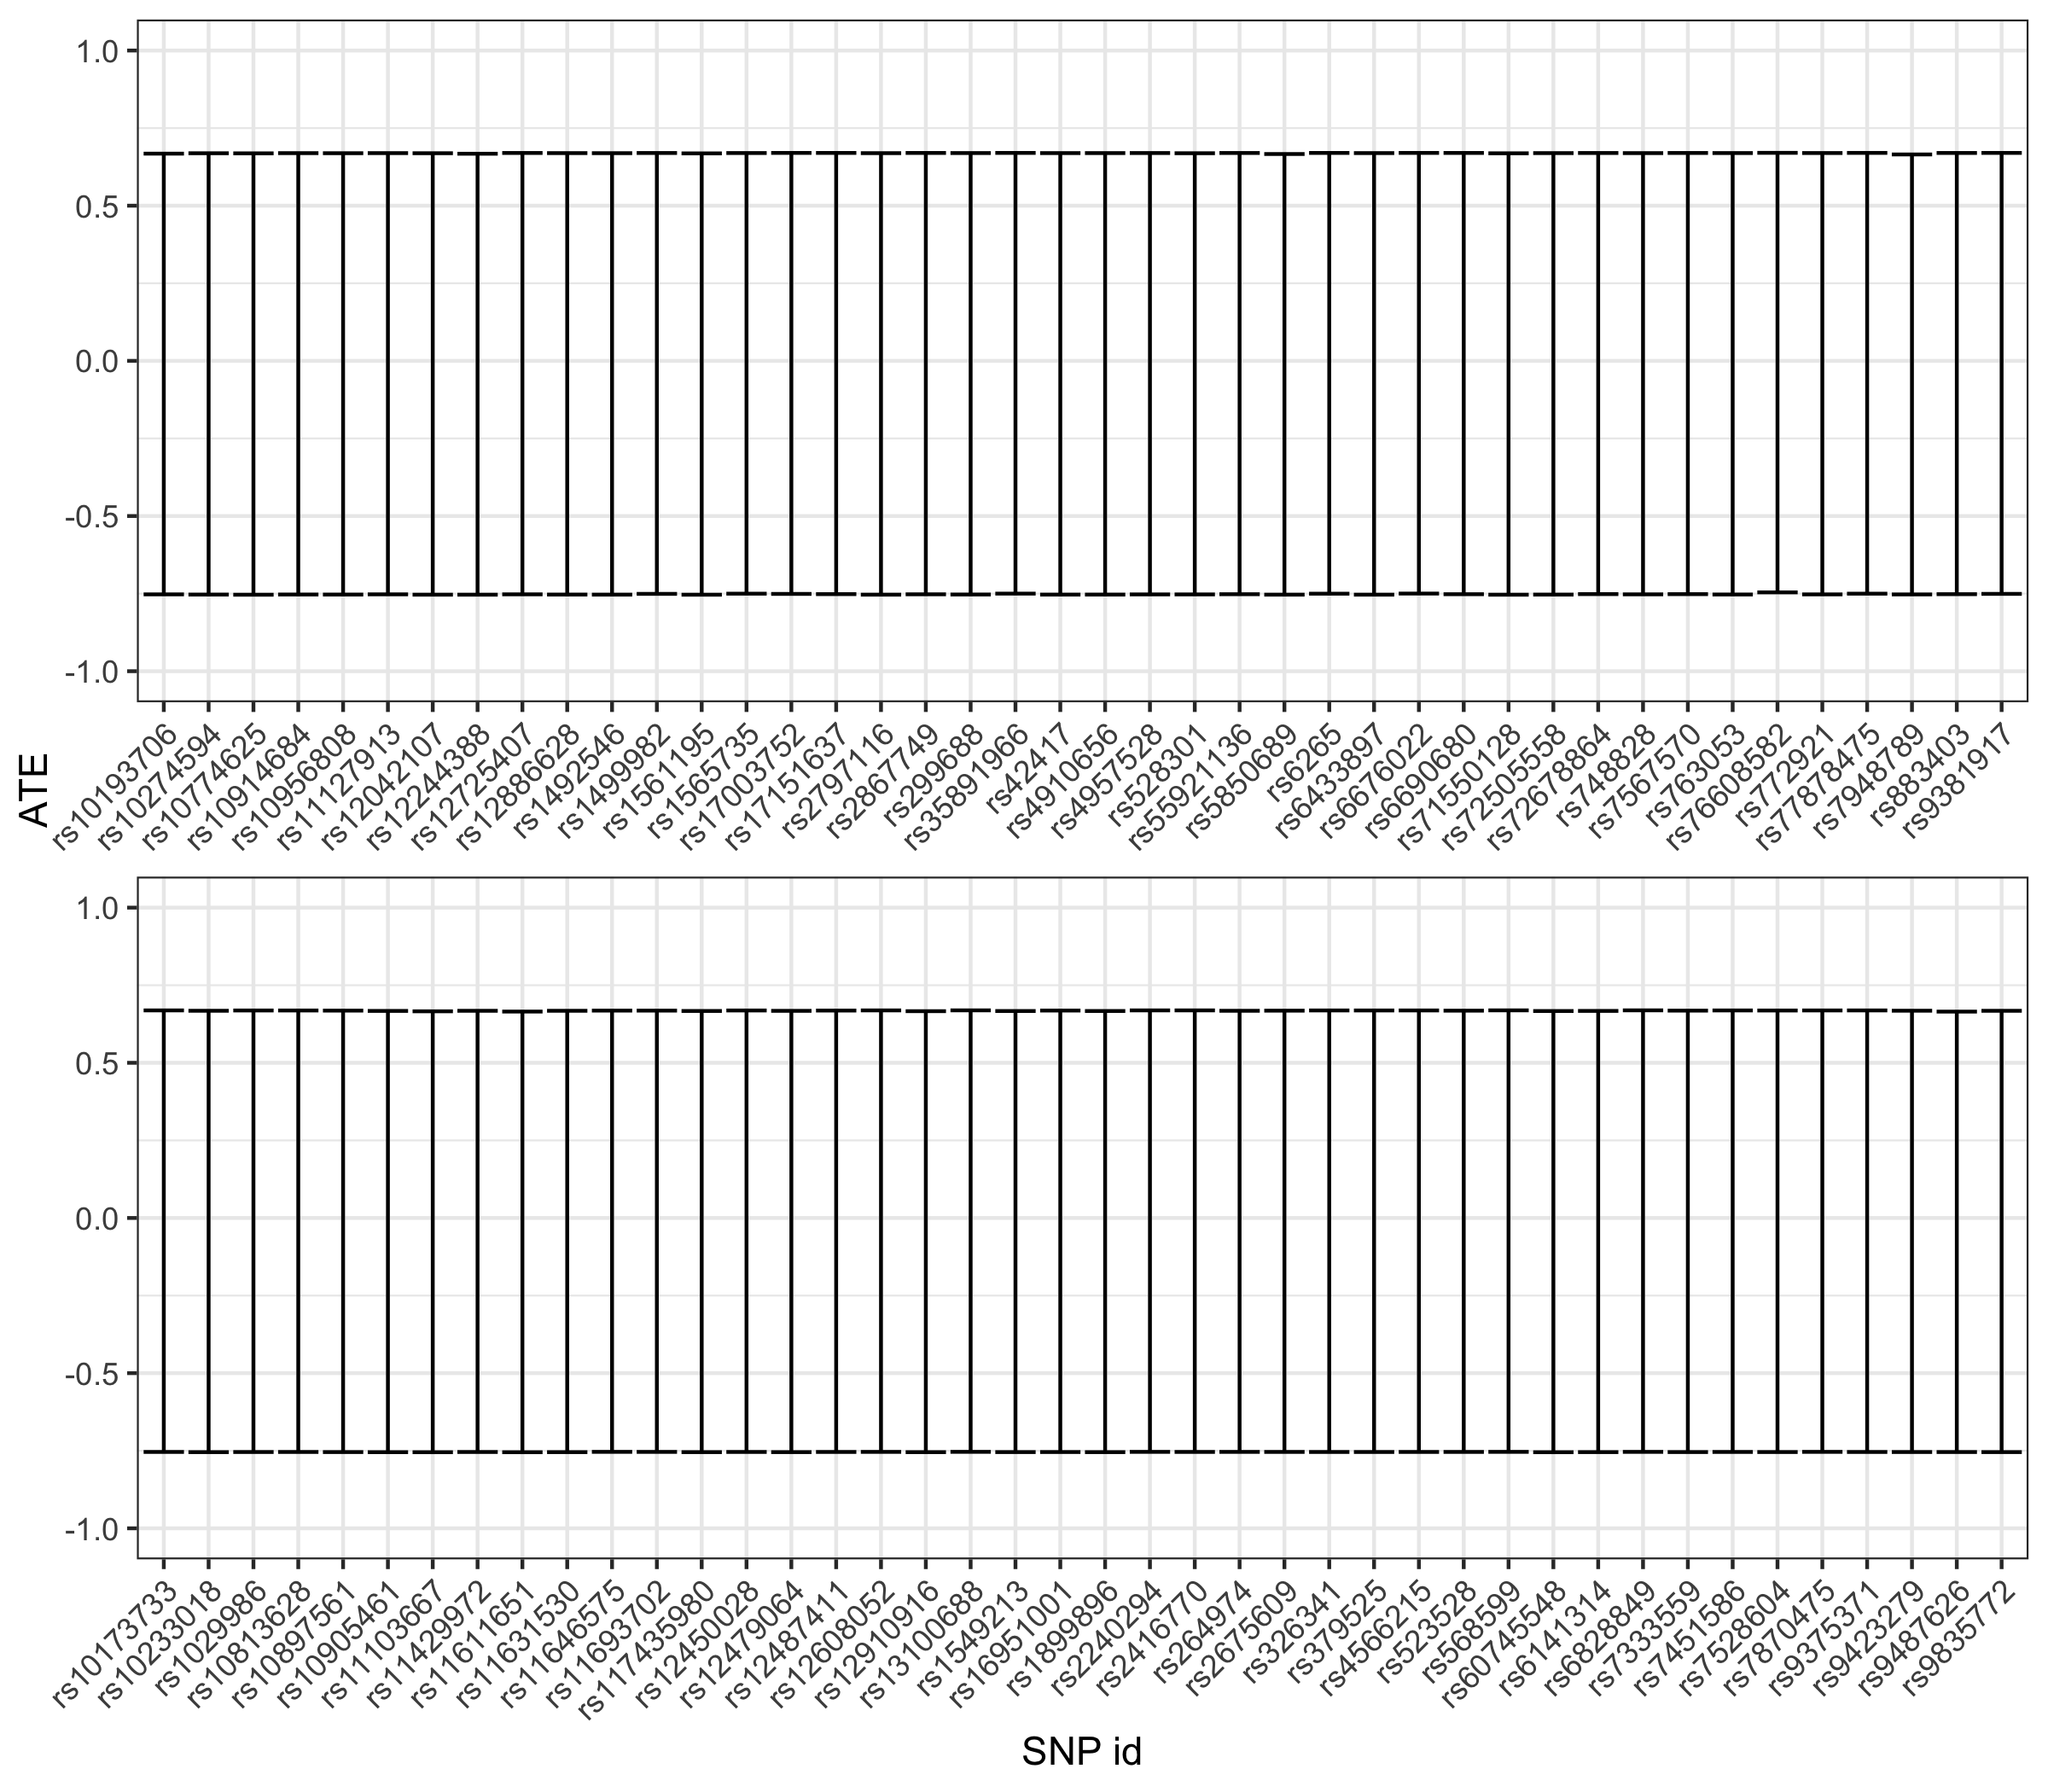
\includegraphics[width = 0.99\linewidth]{/Users/ralphtrane/Documents/RPackages_dev/ACEBounds/figures/example_analyses/smoking_depression_bivaraite_bounds_ukb-d-20116_0_ukb-d-20544_11.png}
  \caption{Non-parametric bounds for the 84 genetic variants identified as potential instruments for the effect of smoking on depression created based on the bivariate probabilities found from GWAS summary statistics.}
  \label{fig:smoking_on_depression_ind_bounds}
\end{figure}

Next, we use our approach to generate plausible one-sample IV bounds and Figure \ref{fig:smoking_on_depression_tri_bounds} shows the resulting bounds \textcolor{red}{can we only present a few of these snps, and put rest in appendix? We can say other bounds are similar to what we have in the main.}. While the one-sample bounds are much narrower than the corresponding two-sample bounds, in line with our expectations, all the one-sample bounds founds contain \(0\). This means that we will not be able to use non-parametric bounds to determine the direction of the ATE of smoking on the chances of developing depression, even if we were to obtain one-sample data. In other words, the bound-based analysis of the MR study may not yield any useful conclusion about the exposure effect.

\clearpage

\begin{sidewaysfigure}
  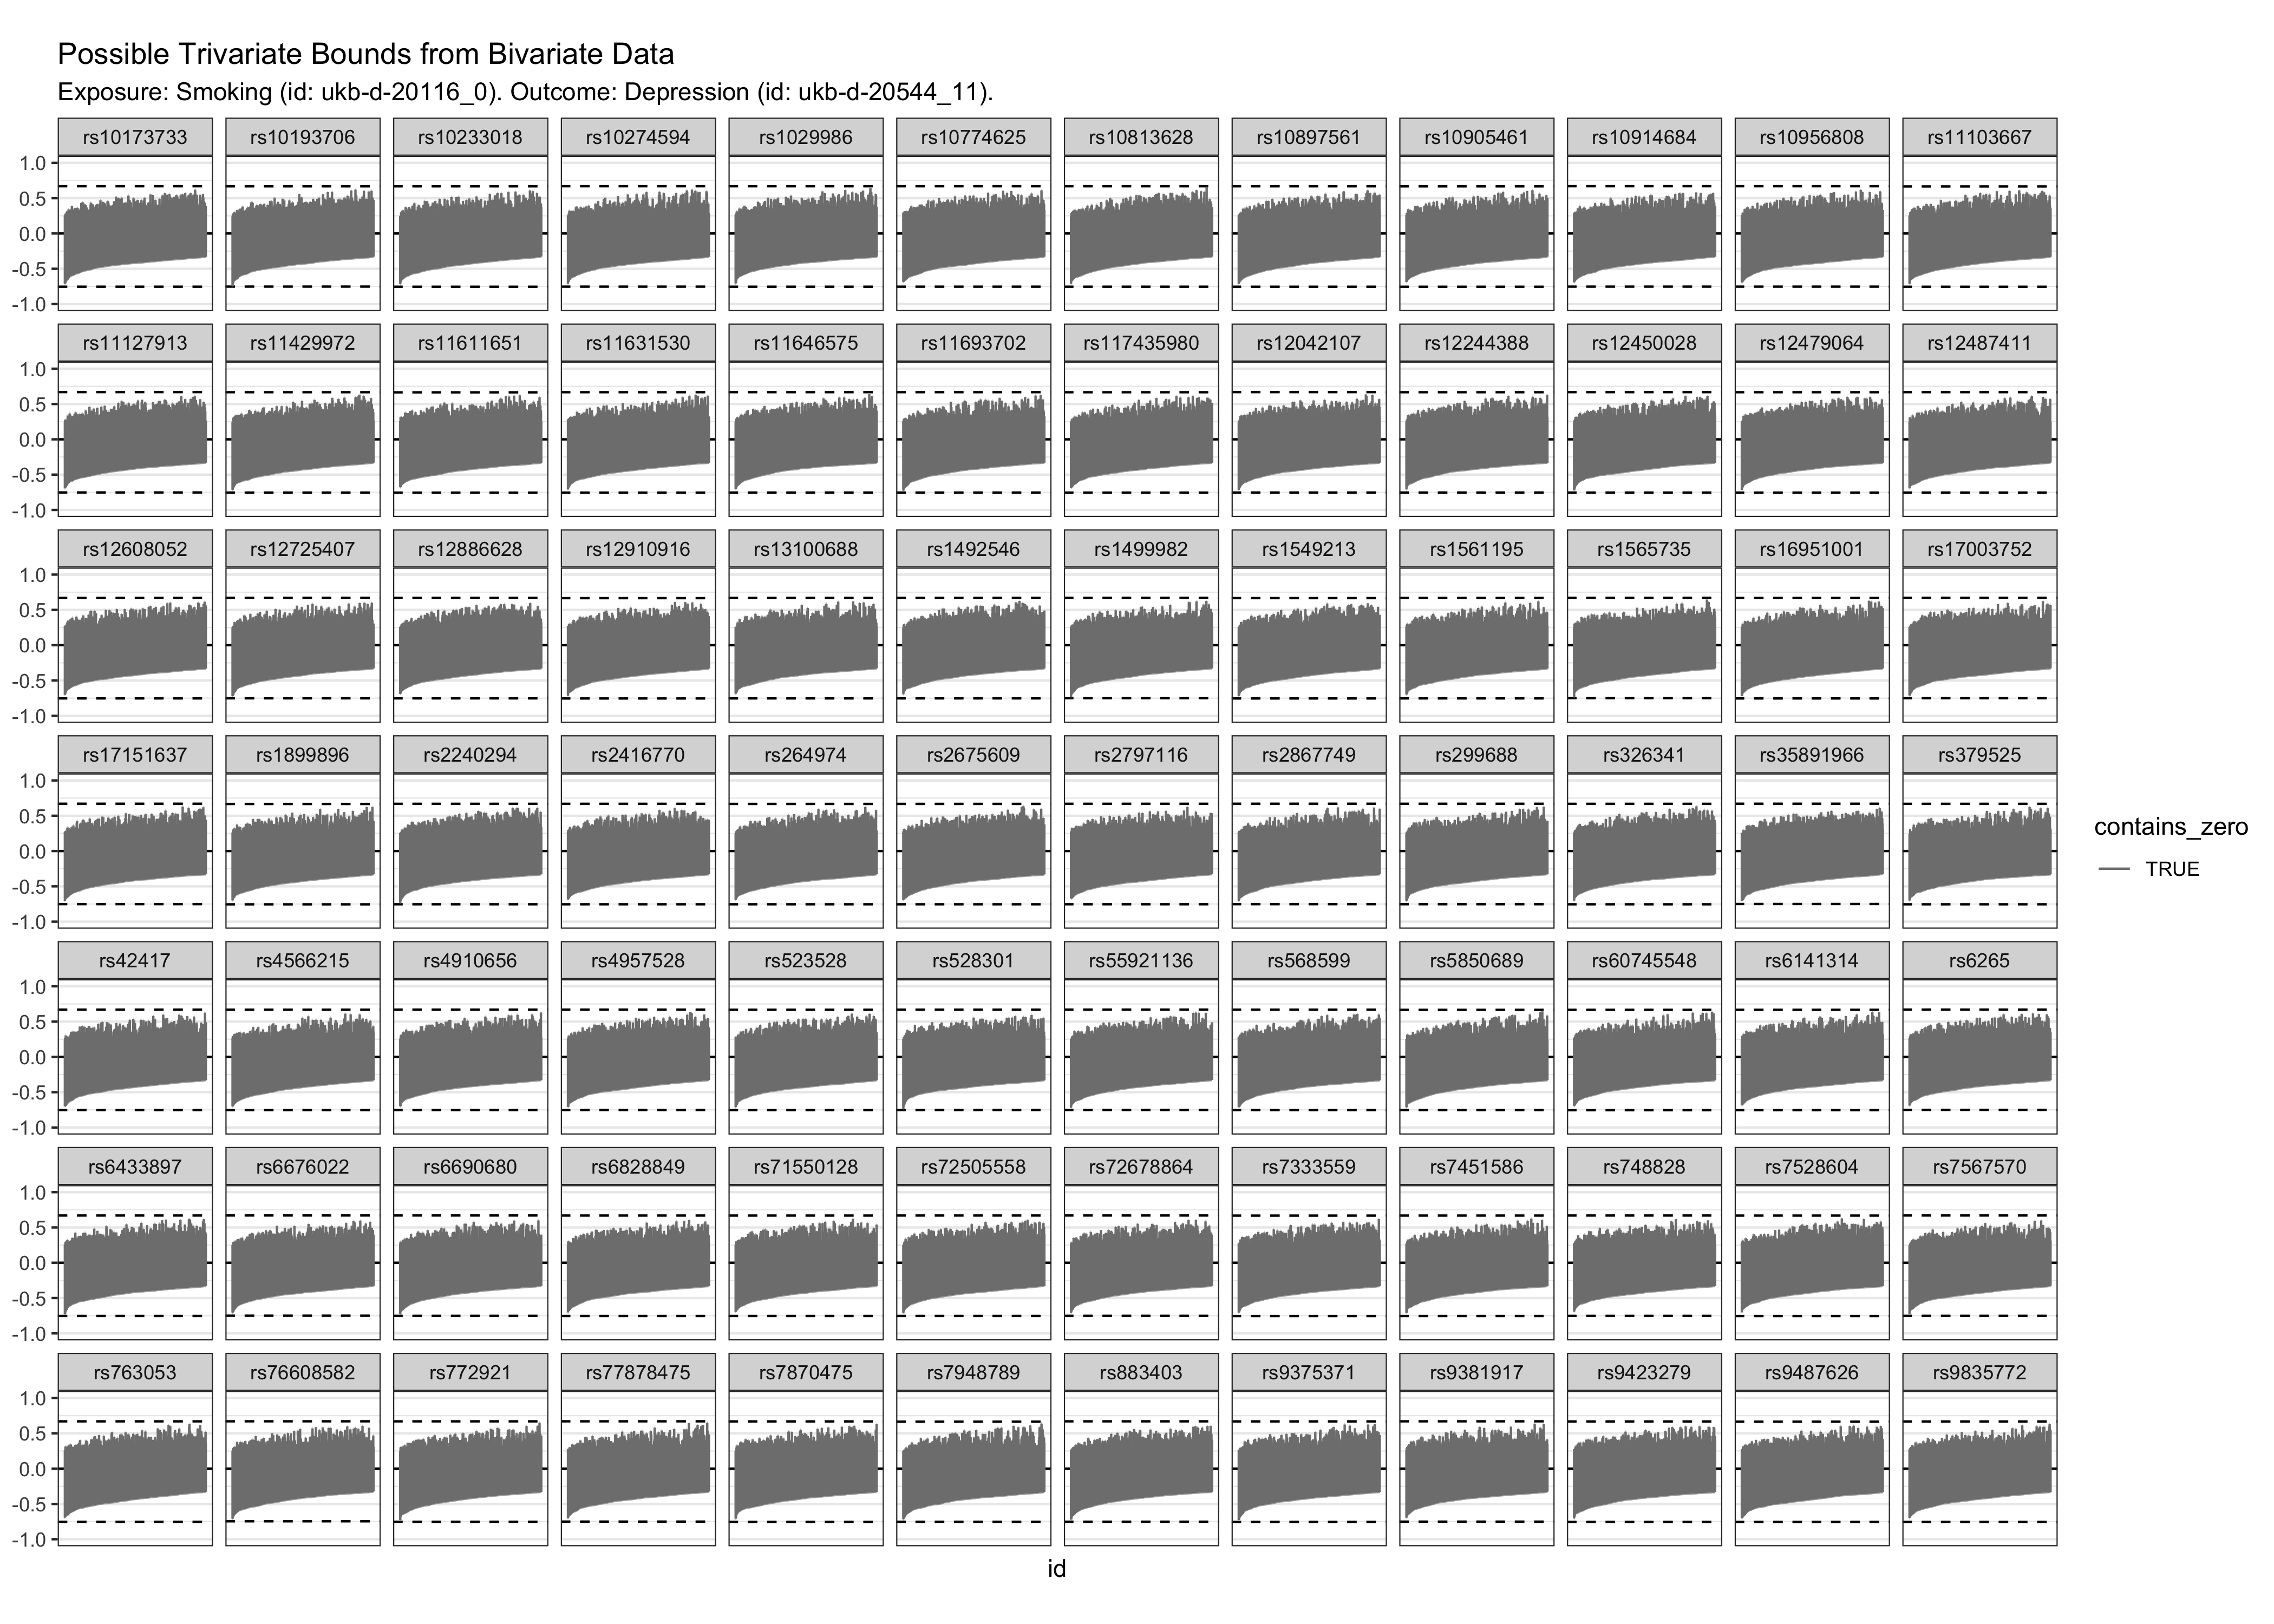
\includegraphics[width = 0.99\textheight]{/Users/ralphtrane/Documents/RPackages_dev/ACEBounds/figures/example_analyses/smoking_depression_individual_SNPs_plot_ukb-d-20116_0_ukb-d-20544_11.png}
    \caption{500 sets of bounds of the average treatment effect of smoking on depression for each of the 84 SNPs. Each bound is based on a set of values for the trivariate distribution randomly sampled. Bounds are color coded to show if they overlap 0 (grey) or do not (red). All bounds overlap 0.}
    \label{fig:smoking_on_depression_tri_bounds}
\end{sidewaysfigure}

\clearpage

\textcolor{red}{fix after discussing what to do with multiple IV section} Aggregating the information from multiple IVs through intersections is a simple idea, but everything we have seen so far points to this not being useful in practice. Figure \ref{fig:smoking_on_depression_intersections} shows the results from doing exactlt this for 9 pairs of SNPs, both when simply creating intersection of the bivariate bounds, and when using our quasi-bayesian approach to estimate the distribution of intersections of bounds from trivariate distributions as described in Section \ref{multiple-iv-case}. Comparing Figure \ref{fig:smoking_on_depression_intersections} to Figure \ref{fig:smoking_on_depression_tri_bounds}, we notice that the intersection bounds are essentially the same width. As for intersections of trivariate bounds, these are narrower than the corresponding intersections of bivariate bounds, but we do not see any scenario where intersections of trivariate bounds would help us determine direction of the ATE. Again, the conclusion is that no sets of trivariate distributions allows us to determine direction of the average treatment effect through the use of non-parametric bounds.

\begin{figure}[H]
  \centering
  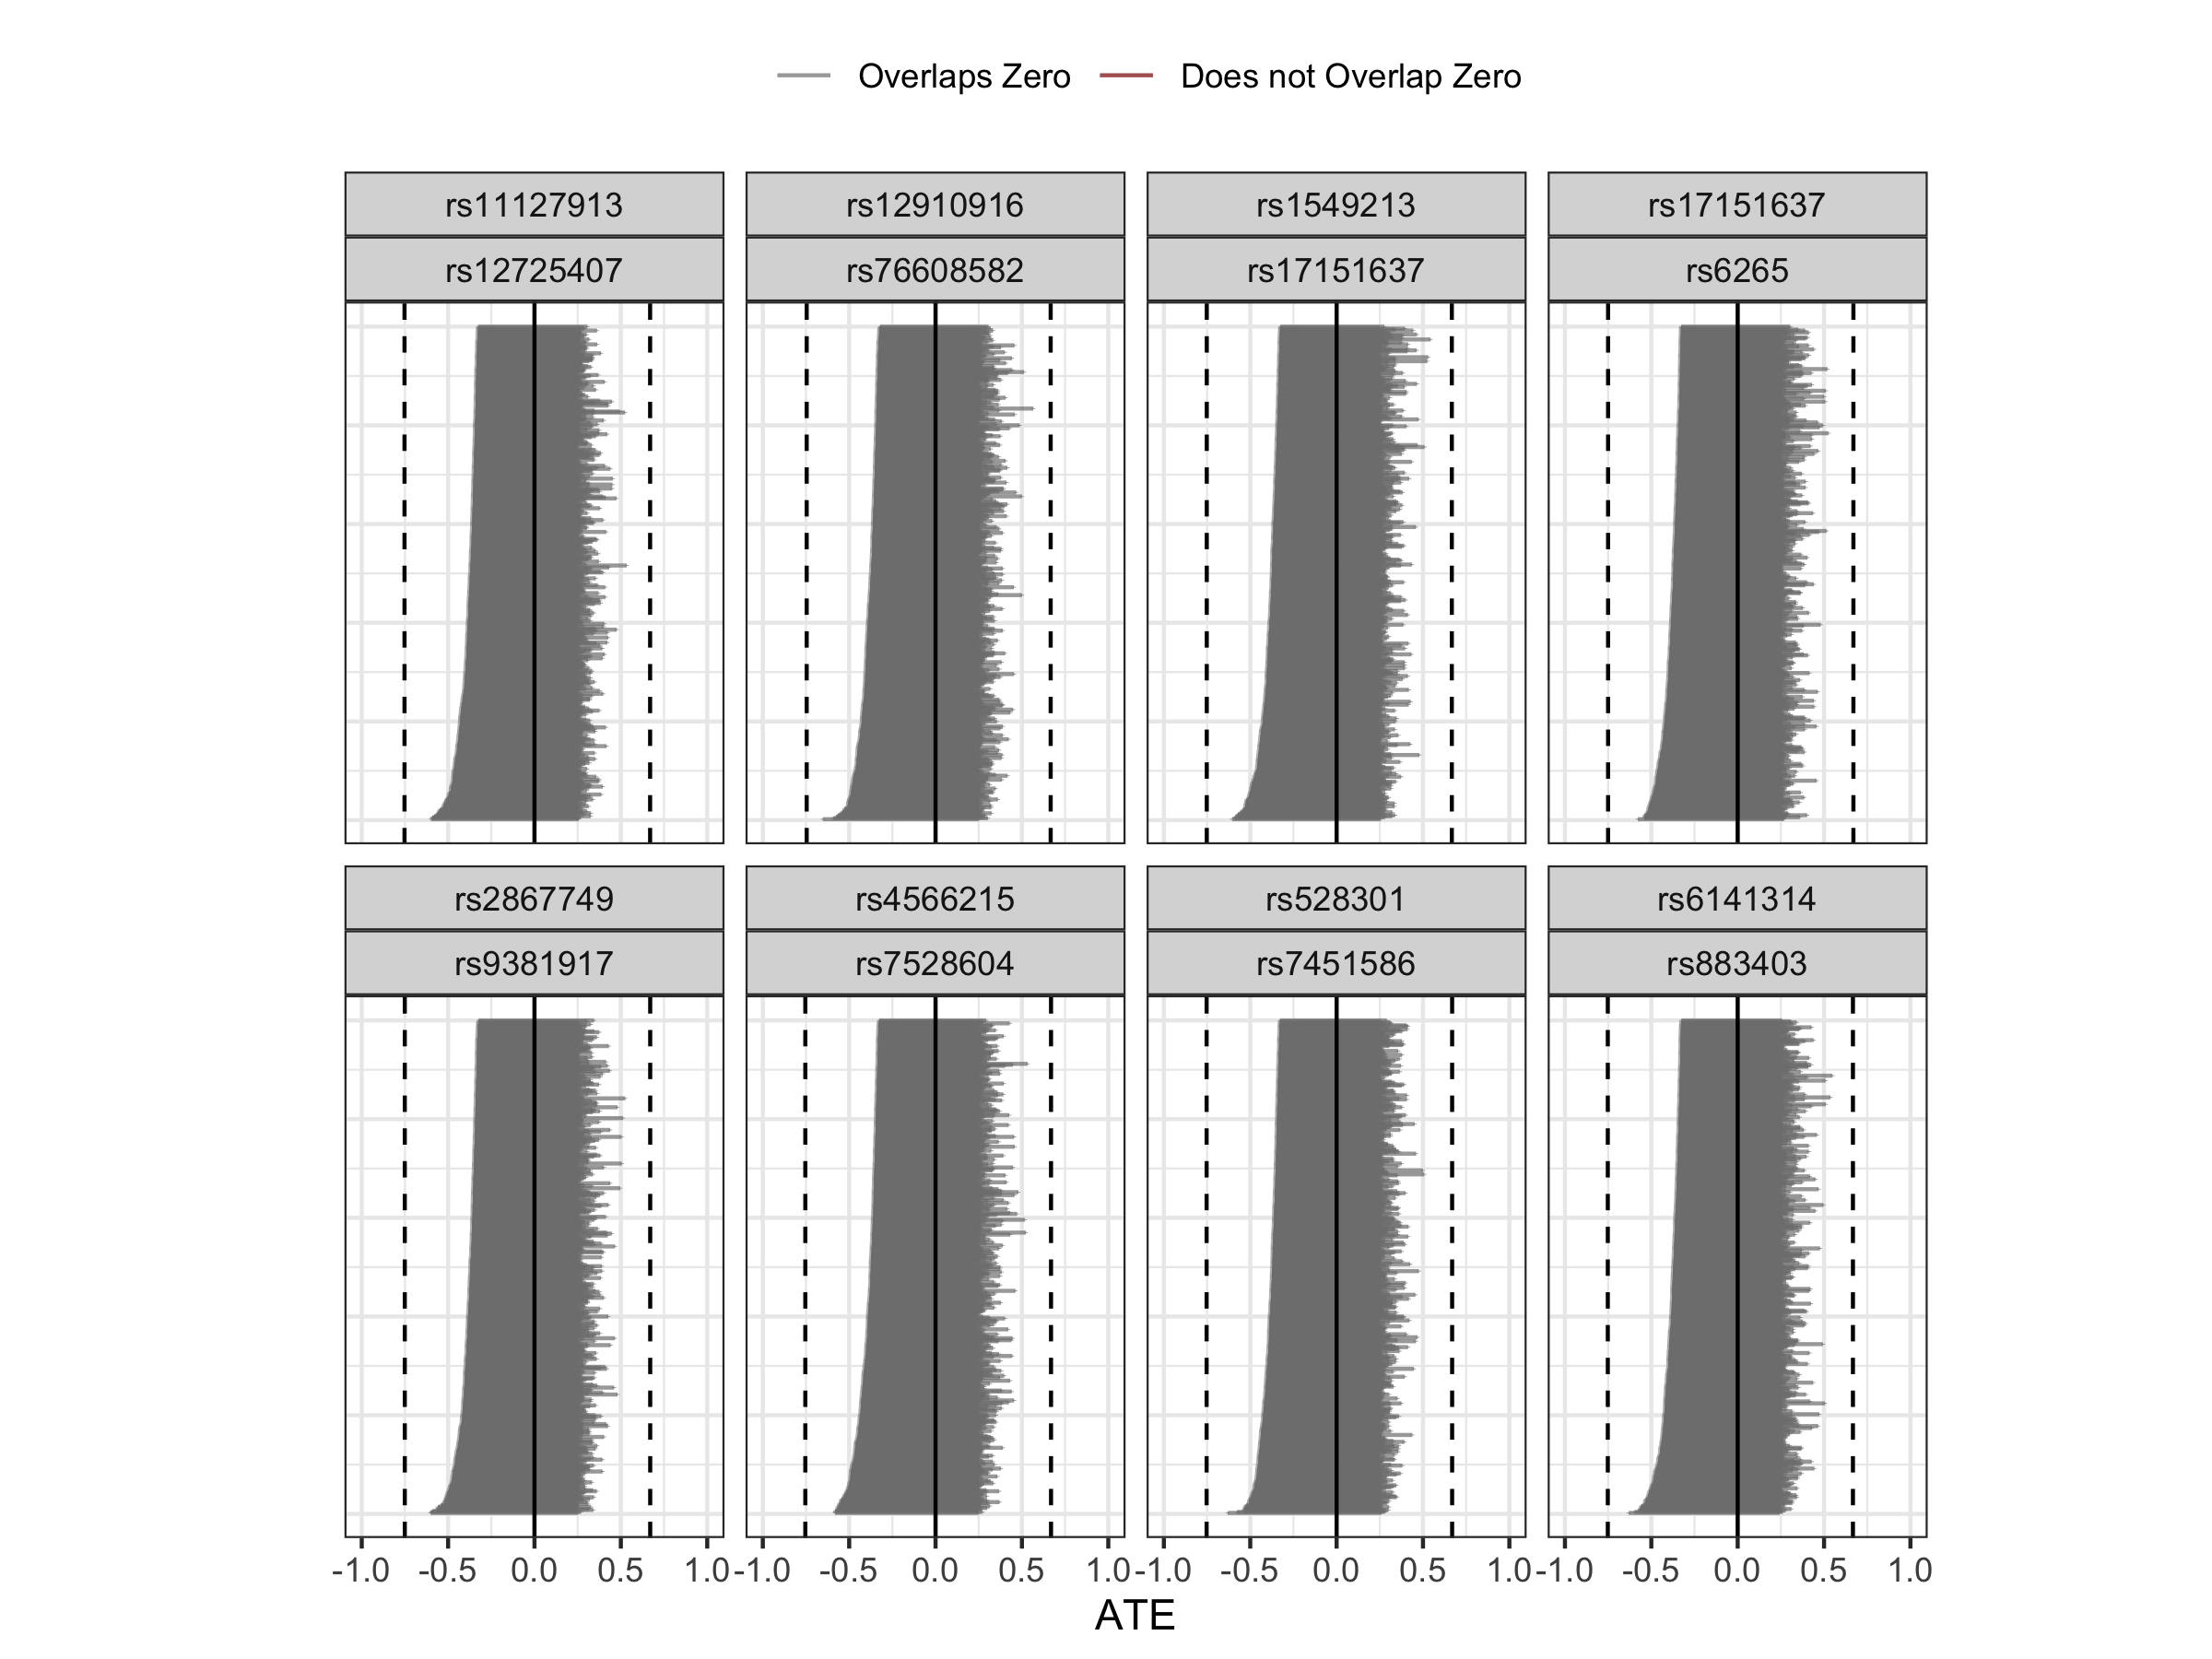
\includegraphics[width = 0.99\linewidth]{/Users/ralphtrane/Documents/RPackages_dev/ACEBounds/figures/example_analyses/smoking_depression_intersection_bounds_plot_ukb-d-20116_0_ukb-d-20544_11.png}
  \caption{Intersection bounds of the average treatment effect of smoking on depression based on randomly sampled trivariate distributions from pairs of SNPs. These 9 pairs were randomly chosen from all possible pairs.}
  \label{fig:smoking_on_depression_intersections}
\end{figure}

\hypertarget{smoking-effect-on-lung-cancer}{%
\subsection{Smoking effect on lung cancer}\label{smoking-effect-on-lung-cancer}}

As a positive control, we consider the effect of smoking on lung cancer. We use the same 84 instruments as in Section \ref{smoking-effect-on-depression} and as expected, the two-sample bounds (Figure \ref{fig:smoking_on_lung_cancer_ind_bounds}) are rather wide; all of them have width greater than 1 and they convey no truly useful information about the ATE. Additionally, even if we were to obtain one-sample data, we will not be able to determine the direction of the ATE (Figure \ref{fig:smoking_on_lung_cancer_tri_bounds}). Aggregating through intersections (Figure \ref{fig:smoking_on_lung_cancer_intersections}) does not lead to real gain in information, even if this is done using bounds based on trivariate distributions.

\begin{figure}[H]
  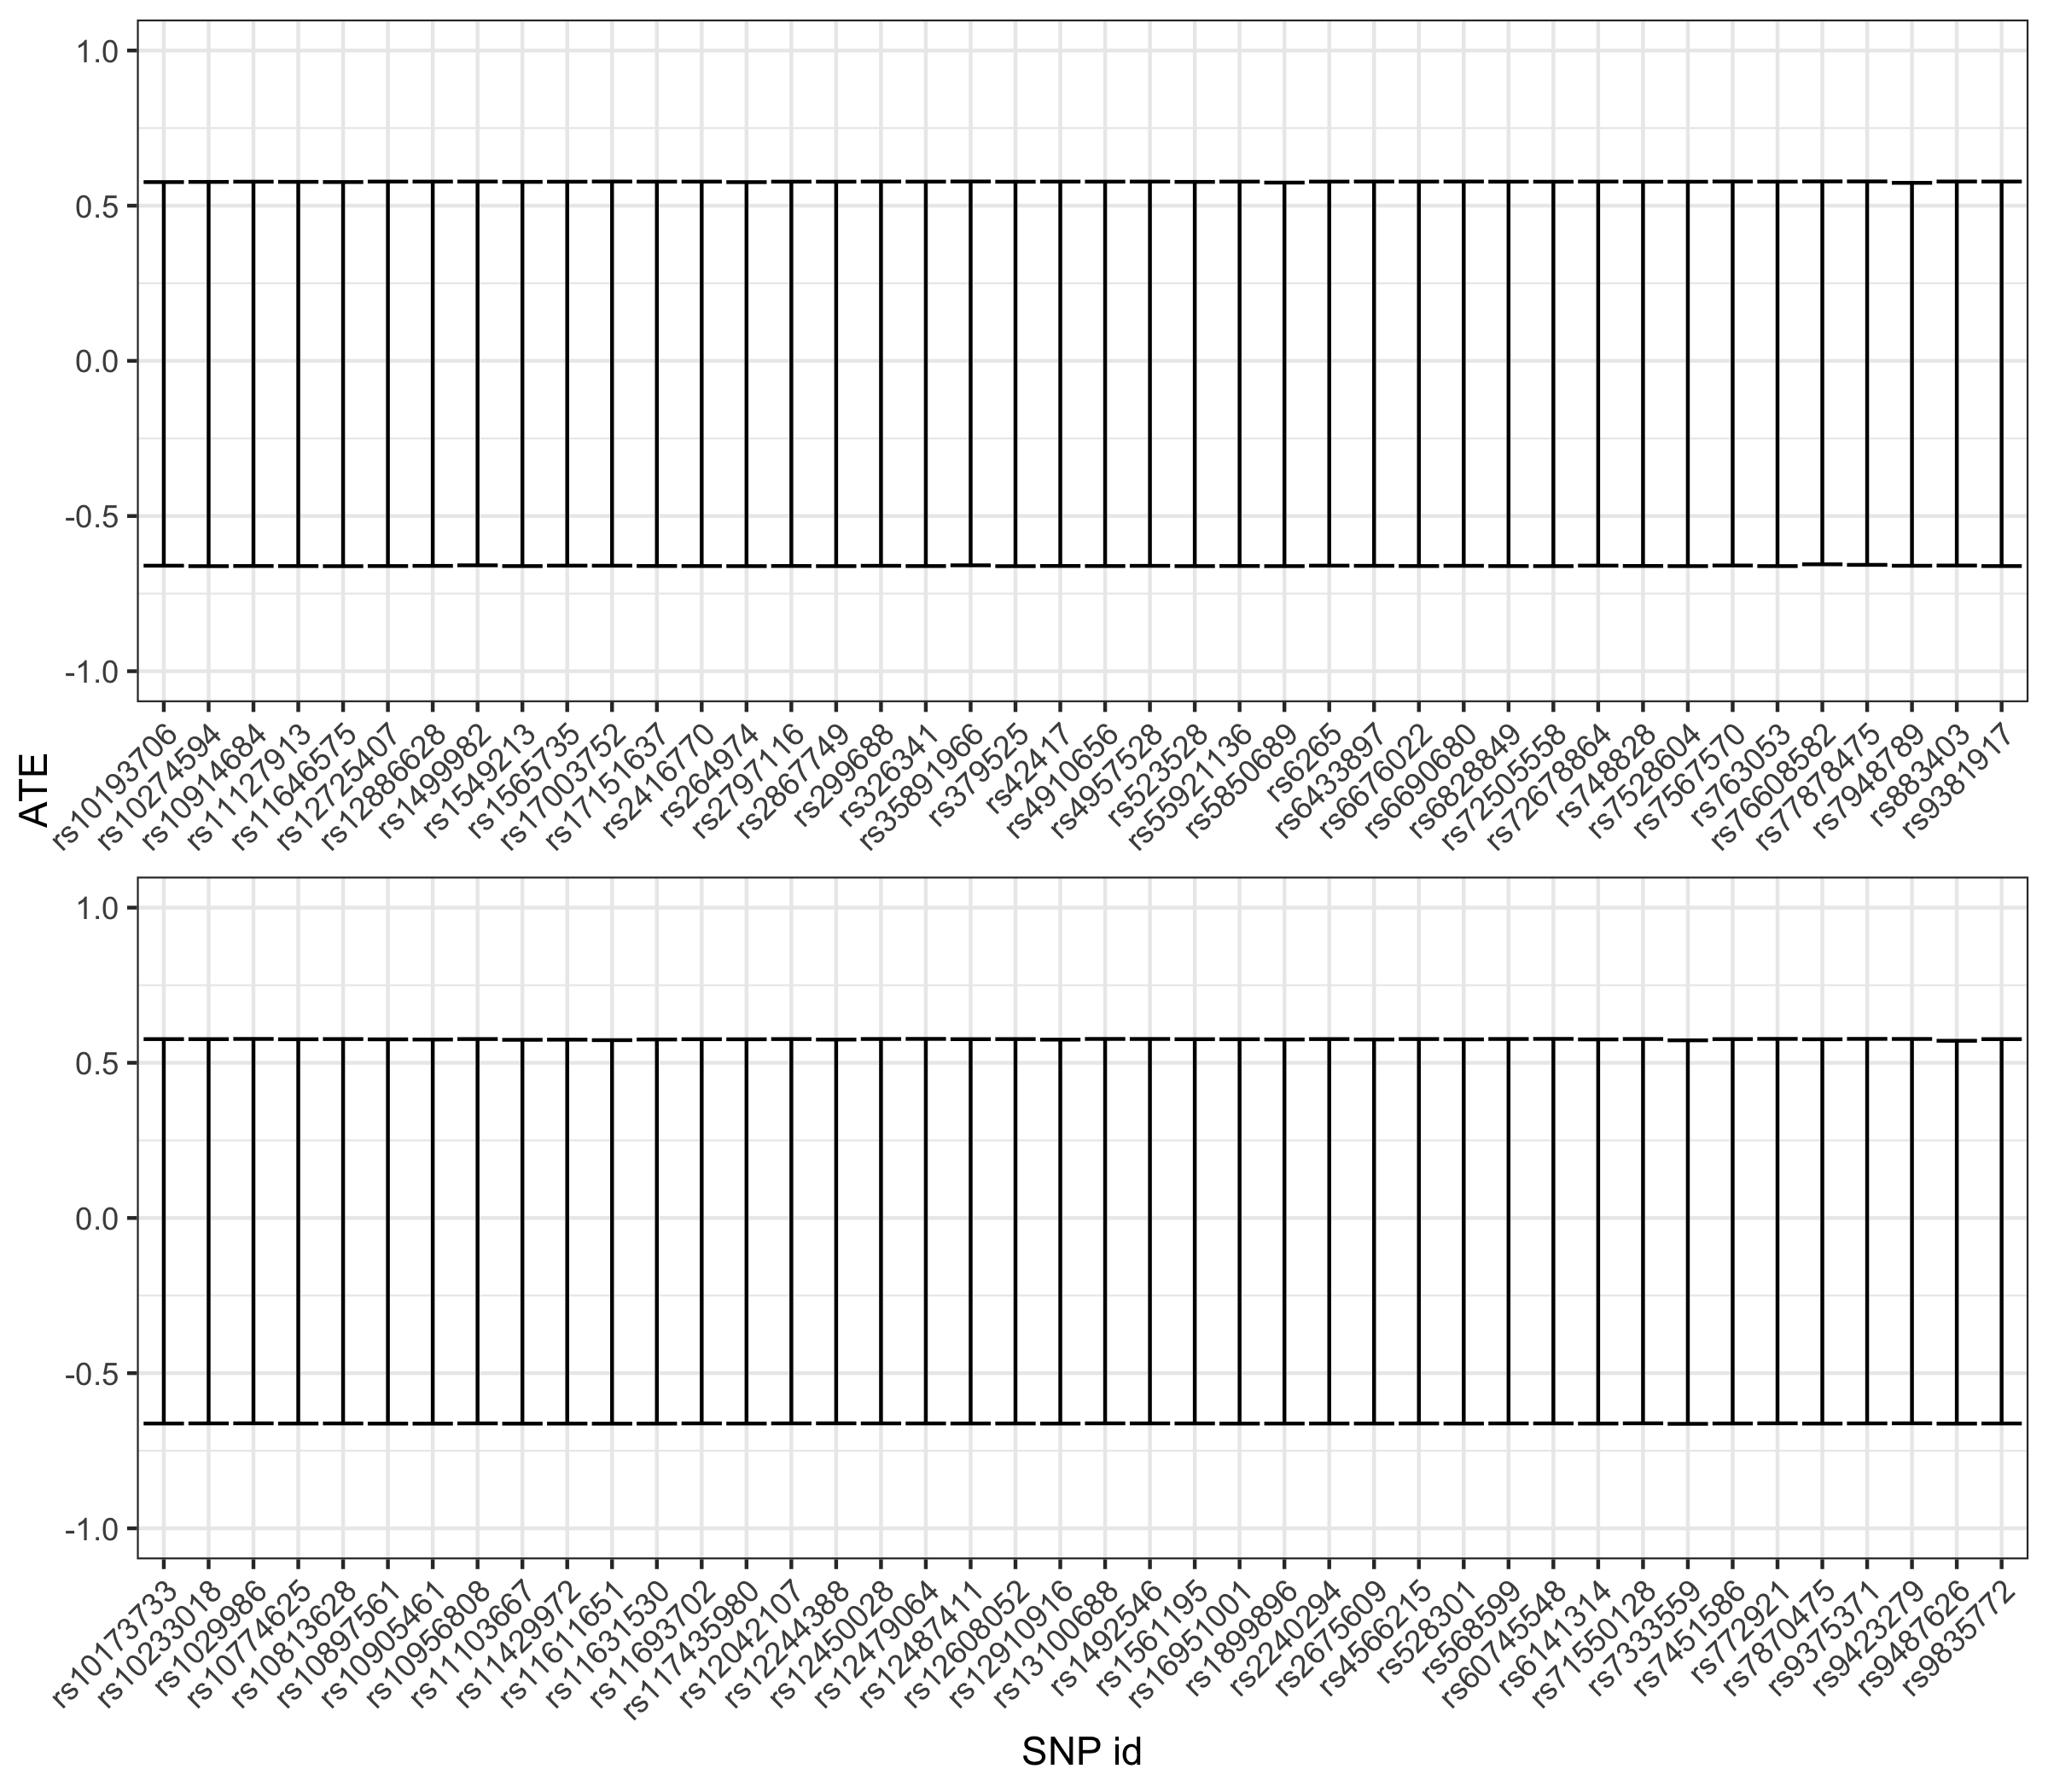
\includegraphics[width = 0.99\linewidth]{/Users/ralphtrane/Documents/RPackages_dev/ACEBounds/figures/example_analyses/smoking_lung_cancer_3_bivaraite_bounds_ukb-d-20116_0_ukb-d-40001_C349.png}
  \caption{Non-parametric bounds on the average treatment effect of smoking on lung cancer.}
  \label{fig:smoking_on_lung_cancer_ind_bounds}
\end{figure}

\clearpage

\begin{sidewaysfigure}
  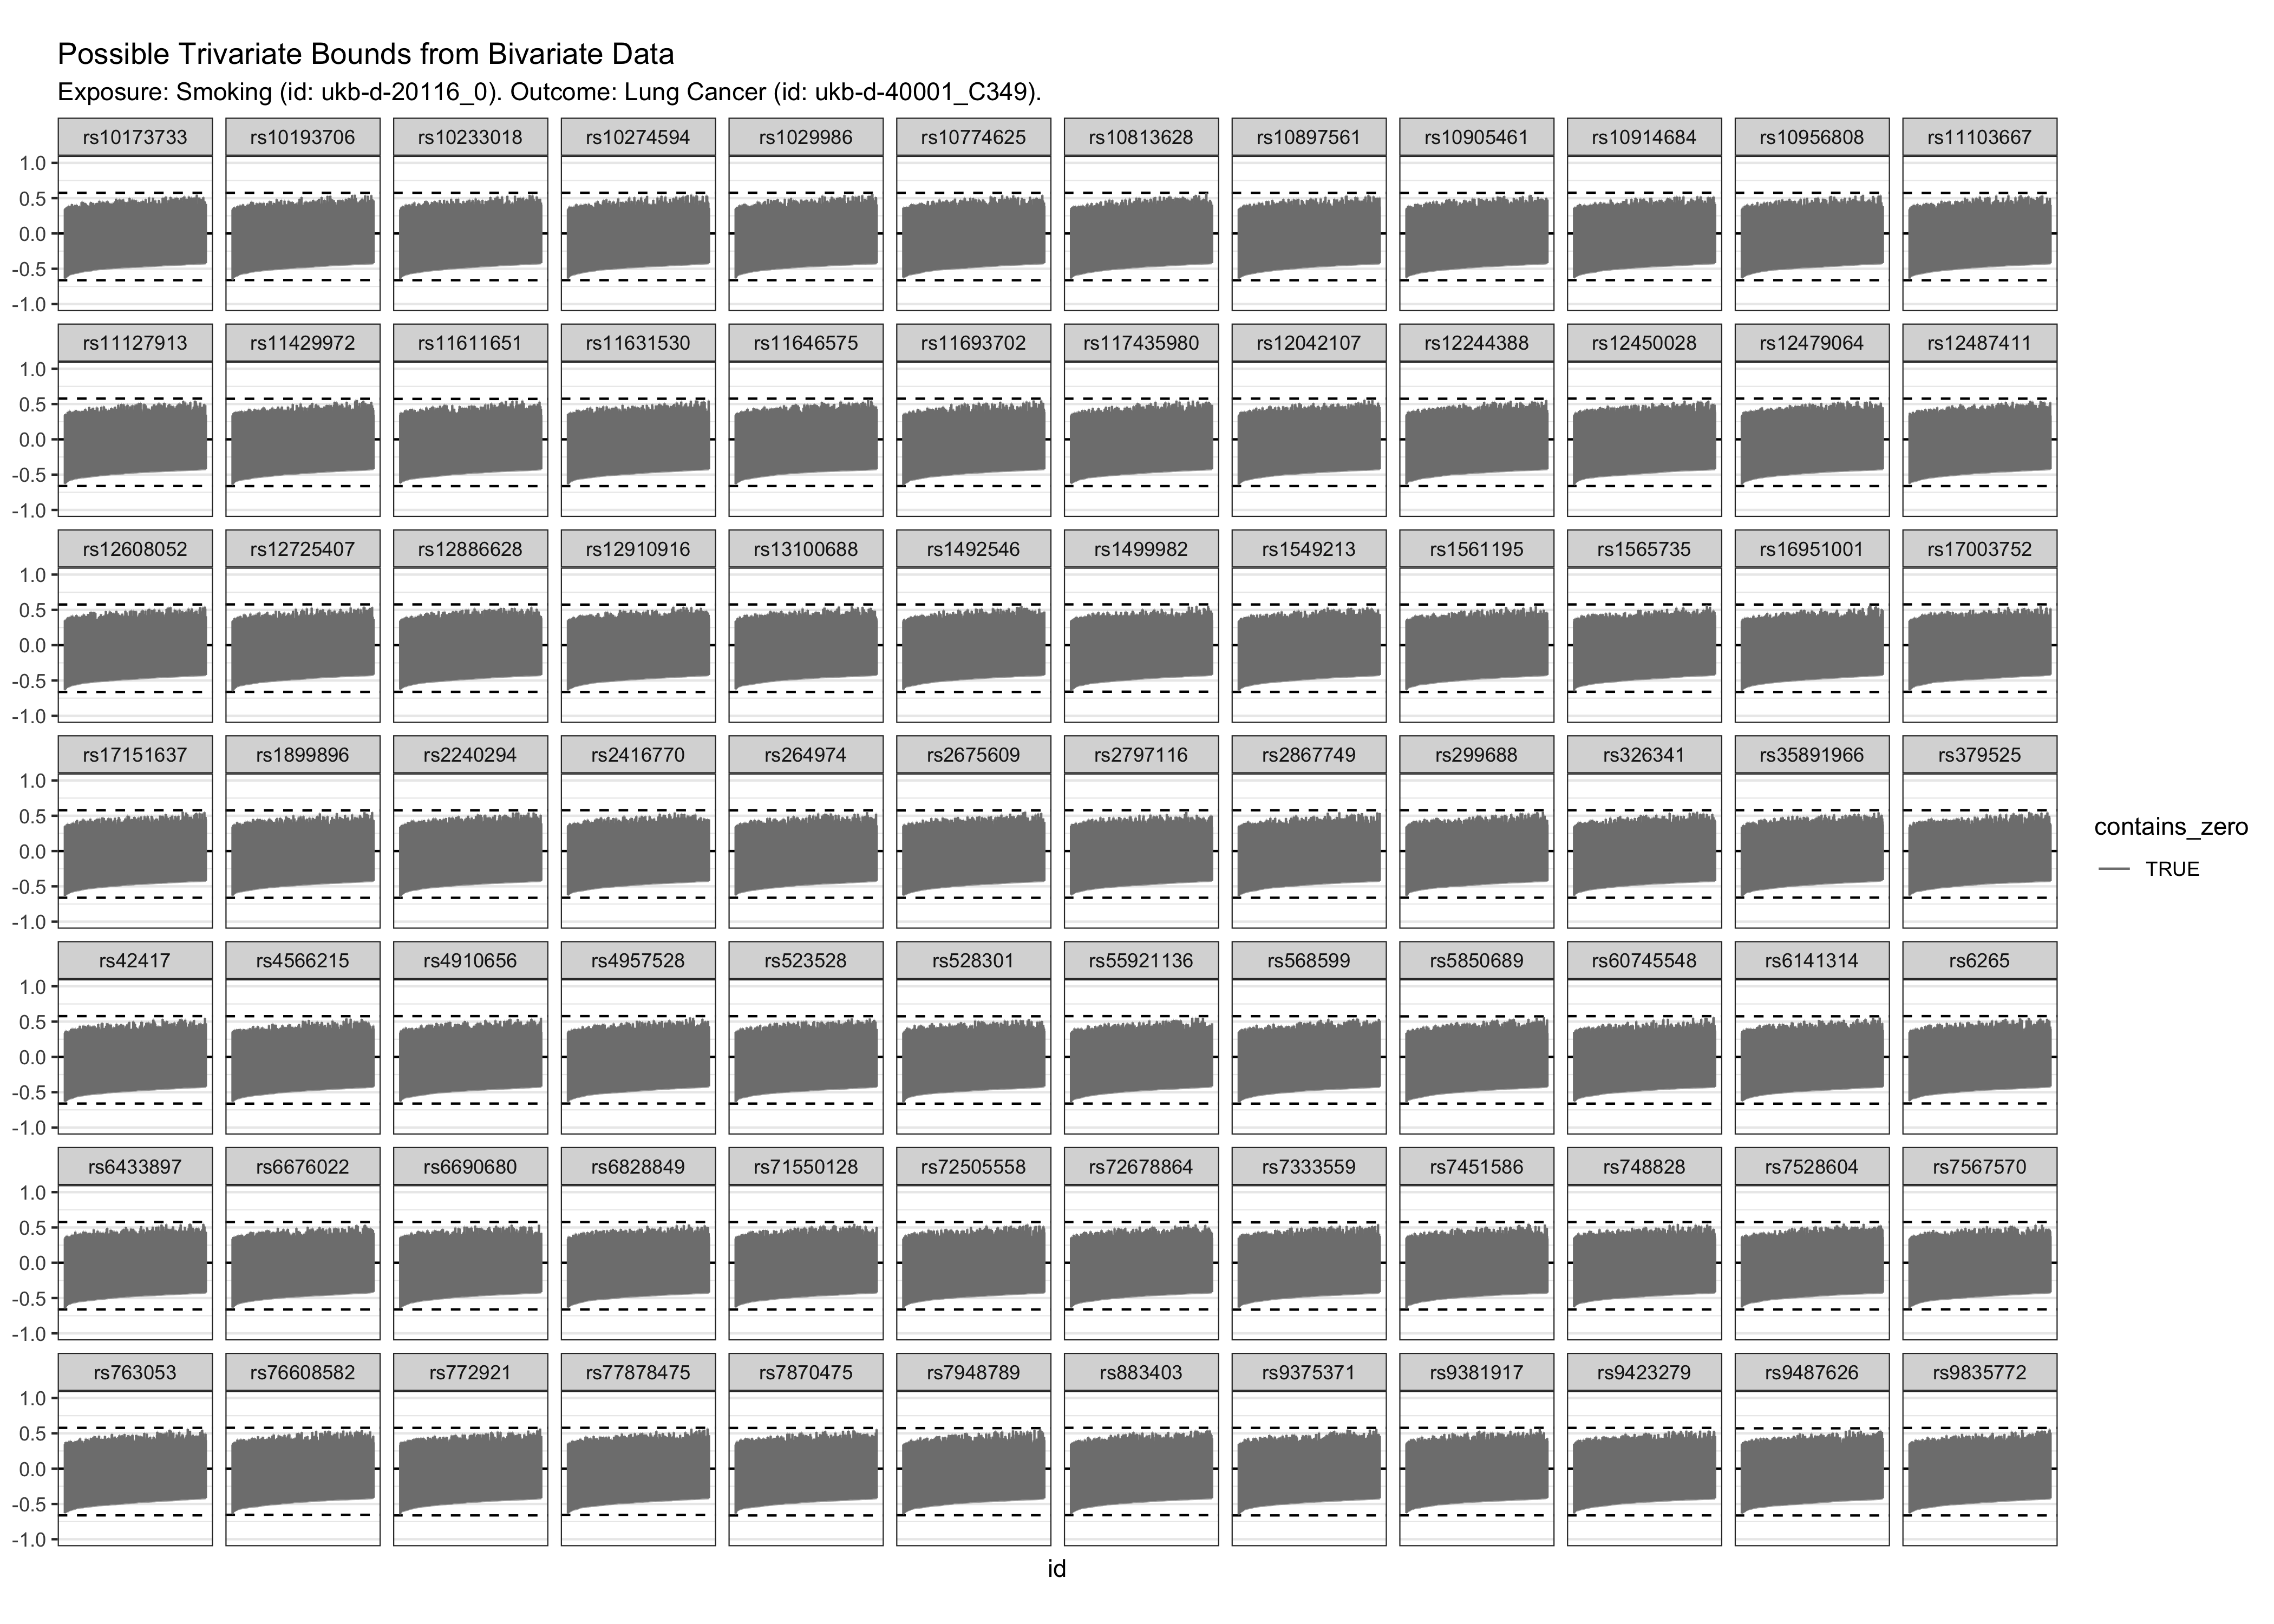
\includegraphics[width = 0.99\textheight]{/Users/ralphtrane/Documents/RPackages_dev/ACEBounds/figures/example_analyses/smoking_lung_cancer_3_individual_SNPs_plot_ukb-d-20116_0_ukb-d-40001_C349.png}
    \caption{500 sets of bounds of the average treatment effect of smoking on lung cancer for each of the 84 SNPs. Each bound is based on a set of values for the trivariate distribution randomyl sampled. Bounds are color coded to show if they overlap 0 (grey) or do not (red). All bounds overlap 0.}
    \label{fig:smoking_on_lung_cancer_tri_bounds}
\end{sidewaysfigure}

\clearpage

\begin{figure}[H]
  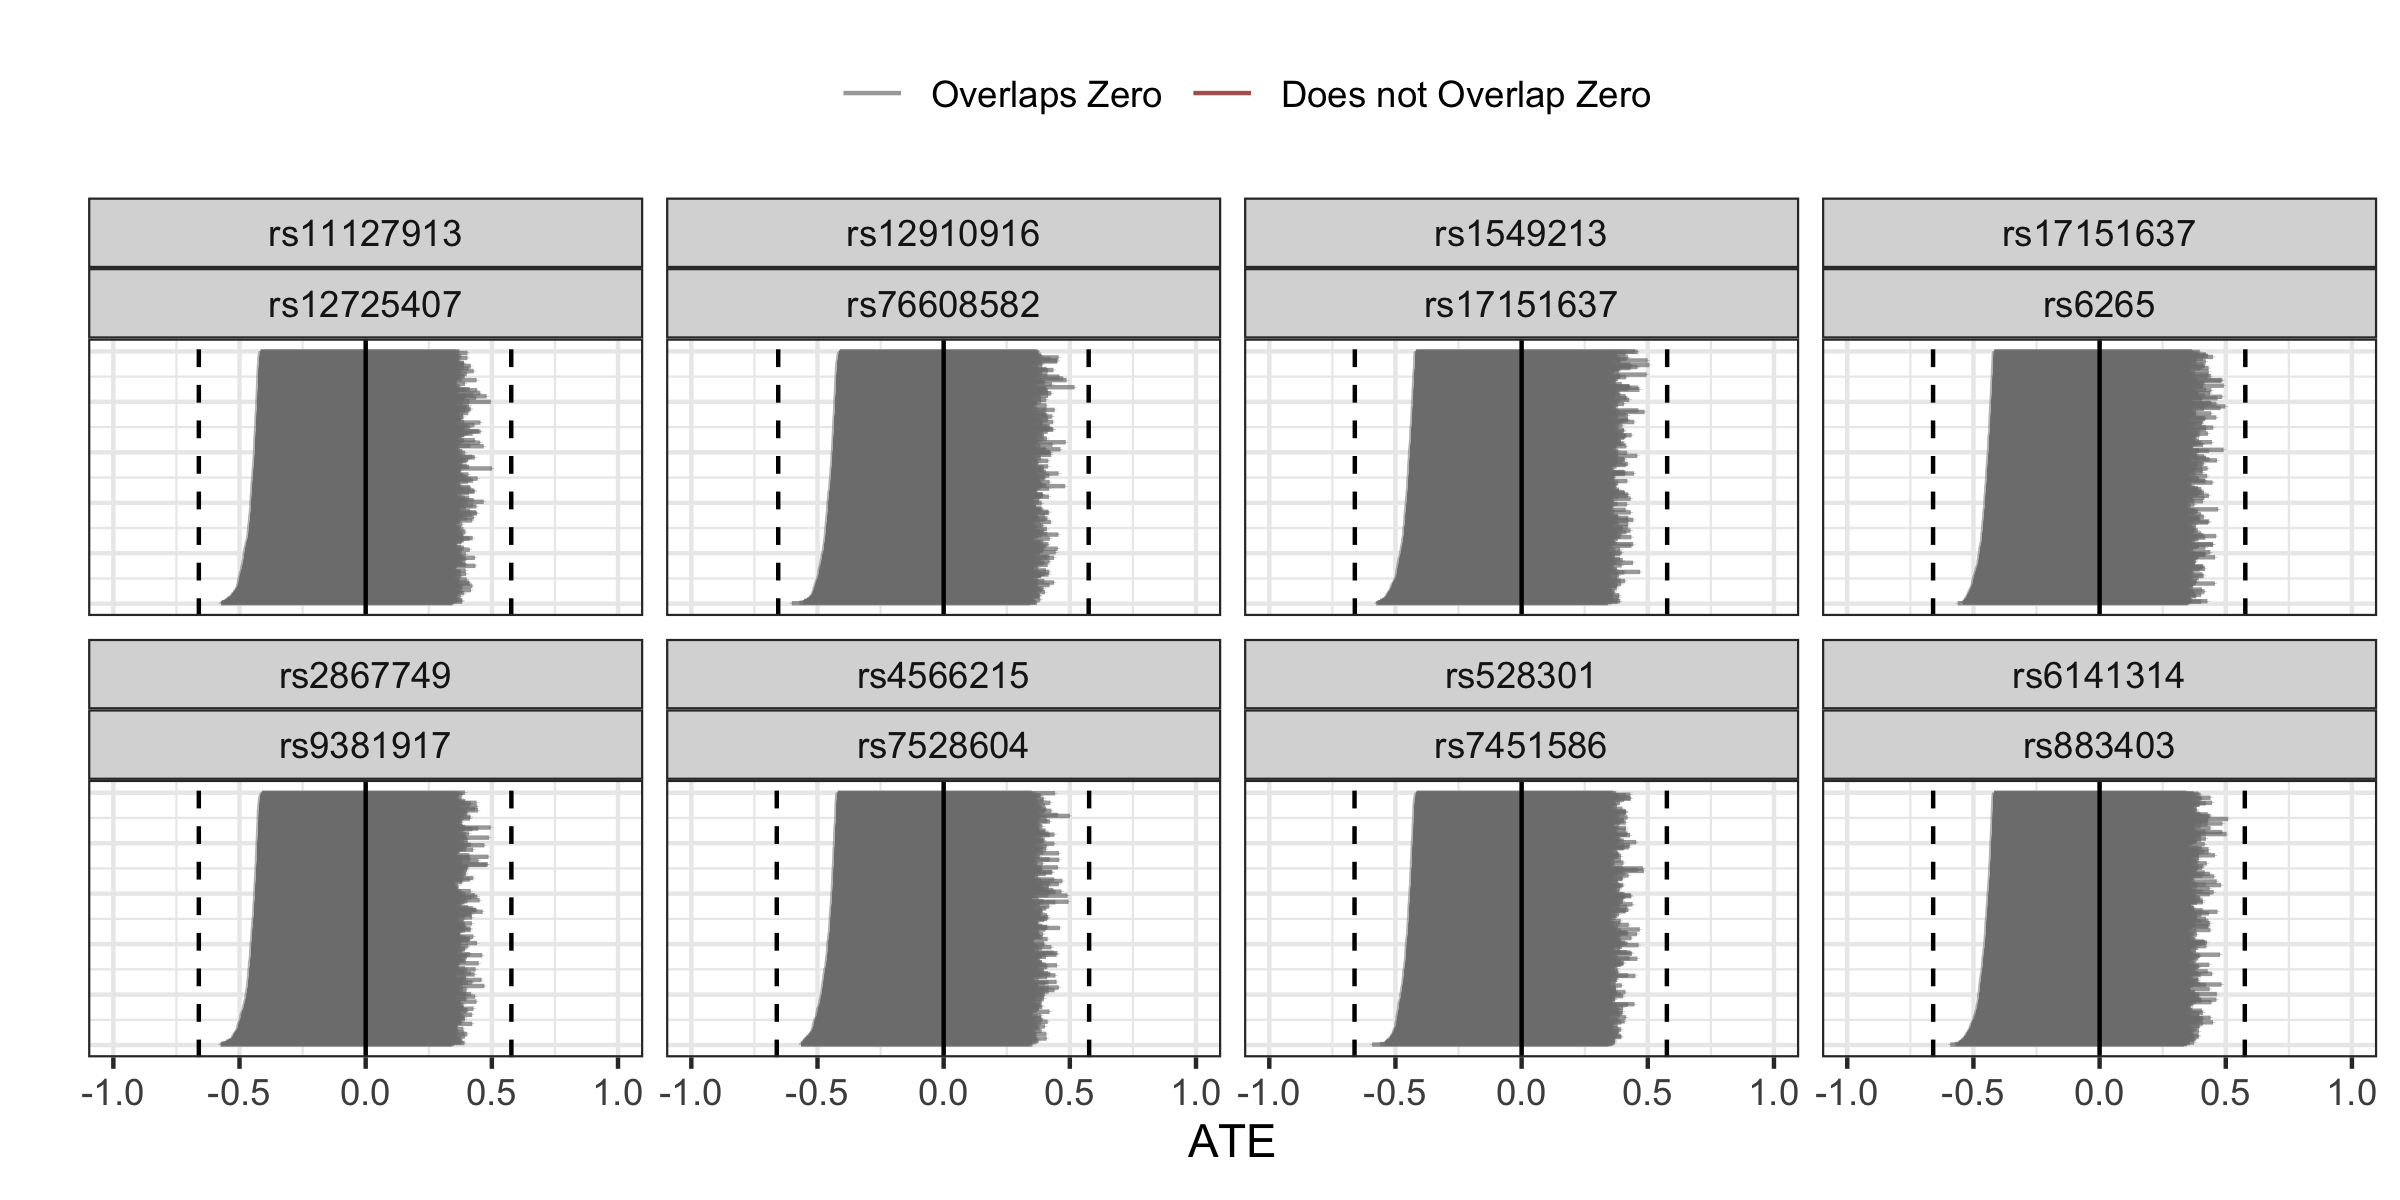
\includegraphics[width = 0.99\linewidth]{/Users/ralphtrane/Documents/RPackages_dev/ACEBounds/figures/example_analyses/smoking_lung_cancer_3_intersection_bounds_plot_ukb-d-20116_0_ukb-d-40001_C349.png}
  \caption{Intersection bounds of the average treatment effect of smoking on lung cancer based on randomly sampled trivariate distributions from pairs of SNPs. These 9 pairs were randomly chosen from all possible pairs.}
  \label{fig:smoking_on_lung_cancer_intersections}
\end{figure}

The result from our positive control is a cause for concern. In particular, it is well established that smoking has a strong causal effect on the chances of developing lung cancer \citep{cornfield_smoking_1959}. The fact that we are unable to say anything about the ATE in this case does not leave much hope in terms of future discoveries based on non-parametric bounds from two-sample MR studies. Even more concerning is the fact that had we obtained one-sample MR data, we would still be unsuccessful in determining the direction of the effect based on a bound-based analysis of the ATE. In short, while non-parametric bounds allow us to make little assumptions about the data and as such, is robust to some common modeling assumptions in MR, they are often too conservative and are not suited for MR studies with many weak instruments.

\newpage

\hypertarget{conclusion-and-practical-considerations}{%
\section{Conclusion and Practical Considerations}\label{conclusion-and-practical-considerations}}

Non-parametric bounds are without a doubt an attractive concept. With a minimal set of assumptions they let us obtain bounds on the average treatment effect. However, as we have seen here, in typical MR studies with two-sample summary data and many weak instruments, bounds may be too uninformative to make meaningful conclusions about the ATE. Specifically, non-parametric bounds in usual one-sample settings data come with very nice guarantees, such as the width always being less than 1. But, in Mendelian randomization analyses with two-sample data, we lose the strong guarantees on the maximum width of the bounds and strong assumptions about the strength of the IV are often required to make sure that the width is less than \(1\). Even aggregating information from many instruments through simple intersections will only be as good as using a single strong instrument.

To address the limitations that the two-sample design has in terms of producing informative bounds, we outline an approach to generate a plausible range of one-sample bounds that are in agreement with the two-sample data at hand. This gives us the opportunity to assess the range of conclusions that can be drawn from bound-based approaches had we had one-sample data. We applied our method to a few different settings of two-sample data and showed the range conclusions about the ATE that can be drawn from it. This exercise also highlighted a significant loss of information in two-sample designs compared to one-sample designs.

\textcolor{red}{need a better way to tie these two paragraphs to rest}
To demonstrate the use of non-parametric bounds in Mendelian randomization analyses, we considered two examples. In the first example, we aimed at finding bounds on the effect of smoking on the chances of developing depression. Unfortunately, all instruments available were very weak with the strongest instrument having a strength of less than \(0.01\). This results in bounds that provide very little information. Our approach suggests that even one-sample bounds would not be able to provide much extra information.

In our second example, we explored the effect of smoking on the chances of developing lung cancer. It has been well established that there is a rather strong causal effect of smoking on the chances of developing lung cancer. Unfortunately, our non-parametric bounds were not able to determine the direction of this effect, and the one-sample bounds once again brought marginal improvement.

\%In this context, it is important to note that the conclusions made about the trivariate distributions only hold if the bivariate probabilities are correct. Whether that is the case here is questionable, as these probabilities are estimated based on logistic regression models.

Using non-parametric bounds in two-sample MR studies seem a promising idea since many MR analysis rely on a host of potentially unjustifiable modeling assumptions. But, as we seen above, the non-parametric nature of these bounds as well as the two-sample design can make these bounds often meaningless in practice. Nevertheless, one potential use case of non-parametric bounds in two-sample MR studies could be when one has prior knowledge about the direction of the effect, but wish to get a better sense of the magnitude. By knowing the sign of the effect a priori, non-parametric bounds can provide an upper limit on this magnitude. This is especially useful in cases where the exposure is known to cause harm or benefit, for example in our smoking lung cancer example where the direction of the effect of smoking on lung cancer is well known and an upper bound on this effect would tell investigators about the maximum possible effect that smoking could have on increasing the propensity of lung cancer.

\newpage

\hypertarget{appendix-appendix}{%
\appendix}


\hypertarget{proof-of-theorem}{%
\section{\texorpdfstring{Proof of Theorem \ref{thm:upperBoundWidth}}{Proof of Theorem }}\label{proof-of-theorem}}

First of all, we note that the bounds found using the approach previously described when we impose both of the mentioned monotonicity assumptions are as follows:

\[
  \begin{aligned}
    &\max
      \begin{Bmatrix}
        -P(Y = 0 | Z = 2) - P(Y = 1 | Z = 0) + P(X = 0 | Z = 0) - P(X = 0 | Z = 2) \\
        P(Y = 0 | Z = 0) - 2\cdot P(Y = 0 | Z = 2) - P(X = 0 | Z = 2) \\
        -P(Y = 0 | Z = 2) - 2\cdot P(Y = 1 | Z = 0) + P(X = 0 | Z = 0)
      \end{Bmatrix} 
      \begin{matrix} (L1) \\ (L2) \\ (L3) \end{matrix}  \\
    &\qquad \qquad \qquad \qquad \qquad\le ATE \le \\
    &\min
      \begin{Bmatrix}
        1 + P(Y = 0 | Z = 0) - P(X = 0 | Z = 0) \\
        1 + P(Y = 0 | Z = 0) - P(Y = 0 | Z = 2) - P(X = 0 | Z = 0) + P(X = 0 | Z = 2) \\
        1 - P(Y = 0 | Z = 2) +  P(X = 0 | Z = 2)
      \end{Bmatrix}
      \begin{matrix} (U1) \\ (U2) \\ (U3) \end{matrix}
  \end{aligned}
\]

This gives us a total of nine different expressions for the width of the bounds. Since we assume monotonicity of the effect of \(Z\) on \(X\), the strength simplifies to \(\text{ST} = P(X = 1 | Z = 2) - P(X = 1 | Z = 0)\).

\textbf{Width = U1 - L1}

If the upper bound is \(U1\), \(U1 \le U2\), which implies \(P(Y = 0 | Z = 2) - P(X = 0 | Z = 2) \le 0\). Therefore,

\[\begin{aligned}
U1 - L1 &= 1 + P(Y = 0 | Z = 0) - P(X = 0 | Z = 0) + P(Y = 0 | Z = 2) + \\
        & \qquad \qquad P(Y = 1 | Z = 0) - P(X = 0 | Z = 0) + P(X = 0 | Z = 2) \\
        &= 2 - ST + P(Y = 0 | Z = 2) - P(X = 0 | Z = 0) \\
        &= 2 - 2\cdot ST + P(Y = 0 | Z = 2) - P(X = 0 | Z = 2) \le 2 - 2\cdot ST.
\end{aligned}\]

\textbf{Width = U2 - L1}

\[\begin{aligned}
U2 - L1 &= 1 + P(Y = 0 | Z = 0) - P(Y = 0 | Z = 2) - P(X = 0 | Z = 0) + P(X = 0 | Z = 2) \\
        &\qquad + P(Y = 0 | Z = 2) + P(Y = 1 | Z = 0) - P(X = 0 | Z = 0) + P(X = 0 | Z = 2) \\
        &= 2 - 2\cdot ST
\end{aligned}\]

\textbf{Width = U3 - L1}

Since the upper bound is \(U3\), \(U3 \le U2\), which implies \(P(X = 0 | Z = 0) - P(Y = 0 | Z = 0) \le 0\). Therefore,

\[\begin{aligned}
U3 - L1 &= 1 - P(Y = 0 | Z = 2) +  P(X = 0 | Z = 2) + P(Y = 0 | Z = 2) + \\
        & \qquad \qquad P(Y = 1 | Z = 0) - P(X = 0 | Z = 0) + P(X = 0 | Z = 2) \\
        &= 1 + P(Y = 1 | Z = 0) - ST + P(X = 0 | Z = 2) \\
        &= 2 - 2\cdot ST + P(X = 0 | Z = 0) - P(Y = 0 | Z = 0) \le 2 - 2 \cdot ST.
\end{aligned}\]

\textbf{Width = U1 - L2}

Since the upper bound is \(U1\), \(P(Y = 0 | Z = 2) \le P(X = 0 | Z = 2)\). Since the lower bound is \(L2\), \(L2 \ge L1\), which gives us \(1 - P(X = 0 | Z = 0) \ge P(Y = 0 | Z = 2)\). Therefore,

\[\begin{aligned}
U1 - L2 &= 1 + P(Y = 0 | Z = 0) - P(X = 0 | Z = 0) - P(Y = 0 | Z = 0) + 2\cdot P(Y = 0 | Z = 2) + P(X = 0 | Z = 2) \\
        &= 1 - ST + 2P(Y = 0 | Z = 2) \\
        &\le 2 - ST - P(X = 0 | Z = 0) + P(X = 0 | Z = 2) = 2 - 2\cdot ST.
\end{aligned}\]

\textbf{Width = U2 - L2}

Since the lower bound is \(L2\), \(1 - P(X = 0 | Z = 0) \ge P(Y = 0 | Z = 2)\). So,

\[\begin{aligned}
U2 - L2 &= 1 - P(X = 0 | Z = 0) + P(X = 0 | Z = 2) + P(Y = 0 | Z = 2) + P(X = 0 | Z = 2) \\
        &= 1 - ST + P(Y = 0 | Z = 2) + P(X = 0 | Z = 2) \\
        &\le 2 - 2\cdot ST.
\end{aligned}\]

\textbf{Width = U3 - L2}

Since the lower bound is \(L2\), \(1 - P(X = 0 | Z = 0) \ge P(Y = 0 | Z = 2)\). Since the upper bound is \(U3\), \(P(X = 0 | Z = 0) \le P(Y = 0 | Z = 0)\). Therefore,

\[\begin{aligned}
U3 - L2 &= 1 - P(Y = 0 | Z = 2) +  P(X = 0 | Z = 2) - P(Y = 0 | Z = 0) + 2\cdot P(Y = 0 | Z = 2) + P(X = 0 | Z = 2) \\
        &= 1 + 2\cdot P(X = 0 | Z = 2) + P(Y = 0 | Z = 2) - P(Y = 0 | Z = 0) \\
        &= 1 - 2\cdot ST + 2 P(X = 0 | Z = 0) + P(Y = 0 | Z = 2) - P(Y = 0 | Z = 0) \\
        &\le 2 - 2\cdot ST
\end{aligned}\]

\textbf{Width = U1 - L3}

Since the upper bound is \(U1\), \(P(Y = 0 | Z = 2) \le P(X = 0 | Z = 2)\). Since the lower bound is \(L3\), \(L3 \ge L1\), which implies \(P(Y = 1 | Z = 0) \le P(X = 0 | Z = 2)\). So,

\[\begin{aligned}
U1 - L3 &= 2 - P(X = 0 | Z = 0) + P(Y = 0 | Z = 2) + P(Y = 1 | Z = 0) - P(X = 0 | Z = 0) \\
        &= 2 - 2\cdot ST - 2\cdot P(X = 0 | Z = 2) + P(Y = 0 | Z = 2) + P(Y = 1 | Z = 0) \\
        &\le 2 - 2\cdot ST
\end{aligned}\]

\textbf{Width = U2 - L3}

Since the lower bound is \(L3\), \(P(Y = 1 | Z = 0) \le P(X = 0 | Z = 2)\)

\[\begin{aligned}
U2 - L3 &= 2 - 2\cdot P(X = 0 | Z = 0) + P(X = 0 | Z = 2) + P(Y = 1 | Z = 0) \\
        &= 2 - ST + P(Y = 1 | Z = 0) - P(X = 0 | Z = 0) \\
        &= 2 - 2\cdot ST + P(Y = 1 | Z = 0) - P(X = 0 | Z = 2) \le 2 - 2\cdot ST
\end{aligned}\]

\textbf{Width = U3 - L3}

Since the lower bound is \(L3\), \(P(Y = 1 | Z = 0) \le P(X = 0 | Z = 2)\). Since the upper bound is \(U3\), \(1 - P(X = 0 | Z = 0) \ge P(Y = 1 | Z = 0)\). Therefore,

\[\begin{aligned}
U3 - L3 &= 1 + P(X = 0 | Z = 2) + 2\cdot P(Y = 1 | Z = 0) - P(X = 0 | Z = 0) \\
        &\le 1 - ST + P(X = 0 | Z = 2) + 1 - P(X = 0 | Z = 0) \\
        &= 2 - 2\cdot ST.
\end{aligned}\]

\newpage

\hypertarget{bounds-on-average-treatment-effect}{%
\section{Bounds on Average Treatment Effect}\label{bounds-on-average-treatment-effect}}

We briefly review the method presented by \citet{ramsahai_causal_2012} to bound the average treatment effect using two-sample summary data. Let \(\vec{\tau}^* = \Big(P(Y = 1 | X = 0, U), P(Y = 1 | X = 1, U), P(X = 1 | Z = 0, U), ..., P(X = 1 | Z = k-1, U)\Big) \in [0,1]^{2+k}\) and \(\vec{v}^* = \Big(P(Y = 0 | Z = 0, U), ..., P(Y = 1 | Z = k-1, U), P(X = 0 | Z = 0, U), ..., P(X = 1 | Z = k-1, U), \alpha^*\Big)\) where

\[
\begin{aligned}
\alpha^* &= P(Y = 1 | X = 1, U) - P(Y = 1 | X = 0, U).
\end{aligned}
\]

Since \(U \perp Z\), \(E_U[P(X = x | Z = z, U)] = P(X = x | Z = z)\) and \(E_U[P(Y = y | Z = z, U)] = P(Y = y | Z = z)\). Let \(\vec{v} = E_U[\vec{v}^*] = \Big(P(Y = 0 | Z = 0), ..., P(Y = 1 | Z = k-1), P(X = 0 | Z = 0), ..., P(X = 1 | Z = k-1), \alpha \Big)\), where

\[
\begin{aligned}
\alpha &= E_U[P(Y = 1 | X = 1, U) - P(Y = 1 | X = 0, U)] \\
       &= E[Y^1] - E[Y^0] = \text{ATE}.
\end{aligned}
\]

Note that while \(\vec{\tau}^*\) and \(\vec{v}^*\) are both entirely unobervable, \(\vec{v}\) consists of \(k\) observable values, and one unobservable value, the ATE.

By the exclusion restriction, we have

\[
P(X = x, Y = y | Z = z, U) = P(Y = 1 | X = x, U) P(X = x | Z = z, U),
\]

which means we can define a mapping \(f:[0,1]^{2+k} \mapsto \mathcal{V}\) such that \(f(\vec{\tau}^*) = \vec{v^*}\) as

\[
f(y_0, y_1, x_0, x_1, ..., x_{k-1}) =
  \begin{pmatrix}
    (1-y_0)\cdot(1-x_0) + (1 - y_1)\cdot x_0 \\
    y_0\cdot (1-x_0) + y_1\cdot x_0 \\
    \vdots \\
    (1-y_0)\cdot(1-x_{k-1}) + (1 - y_1)\cdot x_{k-1} \\
    y_0\cdot (1-x_{k-1}) + y_1\cdot x_{k-1} \\
  \end{pmatrix} \label{eq:f}
\]

We define \(\mathcal{V} = f([0,1]^{2+k})\).

Since \(\vec{v} = E_U[\vec{v}^*]\), \(\vec{v}\) must be a convex combination of \(\vec{v}^*\). Let \(\mathcal{H}\) be the convex hull of \(\mathcal{V}\). Then \(\vec{v}\) will be in \(\mathcal{H}\).

Now, let \(\hat{\mathcal{T}}\) be the set of extreme vertices of \([0,1]^{2+k}\), \(\hat{\mathcal{V}} = f(\hat{\mathcal{T}})\), and \(\hat{\mathcal{H}}\) be the convex hull of \(\hat{\mathcal{V}}\). By Theorem 1 in Appendix B of \citet{ramsahai_causal_2012}, \(\mathcal{H} = \mathcal{\hat{H}}\). This means that \(\vec{v} \in \mathcal{\hat{H}}\). Utilizing a program such as Polymake, we can describe \(\mathcal{H}\) with a set of inequalities, which give us constraints that \(\vec{v}\) must satisfy.

This means that we can obtain inequalities that the components of \(\vec{v}\) must satisfy by describing the extreme vertices of \([0,1]^{2+k}\), map them to \(\mathcal{V}\) using the relatively simple function \(f\), and then use polymake to find inequalities that characterize the convex hull of \(f([0,1])^{2+k}\). This gives us a set of inequalities involving the components of \(\vec{v}\). Some of these will be verifiable, as they will not include the only unobservable quantity \(\alpha\). Others will not be verifiable, but will allow us to obtain bounds on the unobservable quantity \(\alpha\) using the observable entries of \(\vec{v}\).

Following the approach from Ramsahai (2012) as outlined in Section \ref{bounds-on-average-treatment-effect}, we obtain bounds on the average treatment effect from the quantities \(P(X = 1 | Z = z)\) and \(P(Y = 1 | Z = z)\), \(z = 0,1,2\). To do so, we first write down the most extreme values of each of \(P(Y = 1 | X = x, U)\) and \(P(X = x | Z = z, U)\) for all \(x=0,1\), \(z=0,1,2\). Since these are probabilities, the extreme values are \(0\) and \(1\).

\begin{longtable}[]{@{}ccccc@{}}
\caption{Most extreme values of \(P(Y = 1 | X = x, U)\) and \(P(X = 1 | Z = z, U)\). Here, PY1XxU = \(P(Y = 1 | X = x, U)\) and PX1ZzU = \(P(X = 1 | Z = z, U)\).}\tabularnewline
\toprule
\begin{minipage}[b]{0.11\columnwidth}\centering
PY1X0U\strut
\end{minipage} & \begin{minipage}[b]{0.11\columnwidth}\centering
PY1X1U\strut
\end{minipage} & \begin{minipage}[b]{0.11\columnwidth}\centering
PY1Z0U\strut
\end{minipage} & \begin{minipage}[b]{0.11\columnwidth}\centering
PX1Z1U\strut
\end{minipage} & \begin{minipage}[b]{0.11\columnwidth}\centering
PX1Z2U\strut
\end{minipage}\tabularnewline
\midrule
\endfirsthead
\toprule
\begin{minipage}[b]{0.11\columnwidth}\centering
PY1X0U\strut
\end{minipage} & \begin{minipage}[b]{0.11\columnwidth}\centering
PY1X1U\strut
\end{minipage} & \begin{minipage}[b]{0.11\columnwidth}\centering
PY1Z0U\strut
\end{minipage} & \begin{minipage}[b]{0.11\columnwidth}\centering
PX1Z1U\strut
\end{minipage} & \begin{minipage}[b]{0.11\columnwidth}\centering
PX1Z2U\strut
\end{minipage}\tabularnewline
\midrule
\endhead
\begin{minipage}[t]{0.11\columnwidth}\centering
0\strut
\end{minipage} & \begin{minipage}[t]{0.11\columnwidth}\centering
0\strut
\end{minipage} & \begin{minipage}[t]{0.11\columnwidth}\centering
0\strut
\end{minipage} & \begin{minipage}[t]{0.11\columnwidth}\centering
0\strut
\end{minipage} & \begin{minipage}[t]{0.11\columnwidth}\centering
0\strut
\end{minipage}\tabularnewline
\begin{minipage}[t]{0.11\columnwidth}\centering
0\strut
\end{minipage} & \begin{minipage}[t]{0.11\columnwidth}\centering
0\strut
\end{minipage} & \begin{minipage}[t]{0.11\columnwidth}\centering
0\strut
\end{minipage} & \begin{minipage}[t]{0.11\columnwidth}\centering
0\strut
\end{minipage} & \begin{minipage}[t]{0.11\columnwidth}\centering
1\strut
\end{minipage}\tabularnewline
\begin{minipage}[t]{0.11\columnwidth}\centering
0\strut
\end{minipage} & \begin{minipage}[t]{0.11\columnwidth}\centering
0\strut
\end{minipage} & \begin{minipage}[t]{0.11\columnwidth}\centering
0\strut
\end{minipage} & \begin{minipage}[t]{0.11\columnwidth}\centering
1\strut
\end{minipage} & \begin{minipage}[t]{0.11\columnwidth}\centering
0\strut
\end{minipage}\tabularnewline
\begin{minipage}[t]{0.11\columnwidth}\centering
0\strut
\end{minipage} & \begin{minipage}[t]{0.11\columnwidth}\centering
0\strut
\end{minipage} & \begin{minipage}[t]{0.11\columnwidth}\centering
0\strut
\end{minipage} & \begin{minipage}[t]{0.11\columnwidth}\centering
1\strut
\end{minipage} & \begin{minipage}[t]{0.11\columnwidth}\centering
1\strut
\end{minipage}\tabularnewline
\begin{minipage}[t]{0.11\columnwidth}\centering
0\strut
\end{minipage} & \begin{minipage}[t]{0.11\columnwidth}\centering
0\strut
\end{minipage} & \begin{minipage}[t]{0.11\columnwidth}\centering
1\strut
\end{minipage} & \begin{minipage}[t]{0.11\columnwidth}\centering
0\strut
\end{minipage} & \begin{minipage}[t]{0.11\columnwidth}\centering
0\strut
\end{minipage}\tabularnewline
\begin{minipage}[t]{0.11\columnwidth}\centering
0\strut
\end{minipage} & \begin{minipage}[t]{0.11\columnwidth}\centering
0\strut
\end{minipage} & \begin{minipage}[t]{0.11\columnwidth}\centering
1\strut
\end{minipage} & \begin{minipage}[t]{0.11\columnwidth}\centering
0\strut
\end{minipage} & \begin{minipage}[t]{0.11\columnwidth}\centering
1\strut
\end{minipage}\tabularnewline
\begin{minipage}[t]{0.11\columnwidth}\centering
0\strut
\end{minipage} & \begin{minipage}[t]{0.11\columnwidth}\centering
0\strut
\end{minipage} & \begin{minipage}[t]{0.11\columnwidth}\centering
1\strut
\end{minipage} & \begin{minipage}[t]{0.11\columnwidth}\centering
1\strut
\end{minipage} & \begin{minipage}[t]{0.11\columnwidth}\centering
0\strut
\end{minipage}\tabularnewline
\begin{minipage}[t]{0.11\columnwidth}\centering
0\strut
\end{minipage} & \begin{minipage}[t]{0.11\columnwidth}\centering
0\strut
\end{minipage} & \begin{minipage}[t]{0.11\columnwidth}\centering
1\strut
\end{minipage} & \begin{minipage}[t]{0.11\columnwidth}\centering
1\strut
\end{minipage} & \begin{minipage}[t]{0.11\columnwidth}\centering
1\strut
\end{minipage}\tabularnewline
\begin{minipage}[t]{0.11\columnwidth}\centering
0\strut
\end{minipage} & \begin{minipage}[t]{0.11\columnwidth}\centering
1\strut
\end{minipage} & \begin{minipage}[t]{0.11\columnwidth}\centering
0\strut
\end{minipage} & \begin{minipage}[t]{0.11\columnwidth}\centering
0\strut
\end{minipage} & \begin{minipage}[t]{0.11\columnwidth}\centering
0\strut
\end{minipage}\tabularnewline
\begin{minipage}[t]{0.11\columnwidth}\centering
0\strut
\end{minipage} & \begin{minipage}[t]{0.11\columnwidth}\centering
1\strut
\end{minipage} & \begin{minipage}[t]{0.11\columnwidth}\centering
0\strut
\end{minipage} & \begin{minipage}[t]{0.11\columnwidth}\centering
0\strut
\end{minipage} & \begin{minipage}[t]{0.11\columnwidth}\centering
1\strut
\end{minipage}\tabularnewline
\begin{minipage}[t]{0.11\columnwidth}\centering
0\strut
\end{minipage} & \begin{minipage}[t]{0.11\columnwidth}\centering
1\strut
\end{minipage} & \begin{minipage}[t]{0.11\columnwidth}\centering
0\strut
\end{minipage} & \begin{minipage}[t]{0.11\columnwidth}\centering
1\strut
\end{minipage} & \begin{minipage}[t]{0.11\columnwidth}\centering
0\strut
\end{minipage}\tabularnewline
\begin{minipage}[t]{0.11\columnwidth}\centering
0\strut
\end{minipage} & \begin{minipage}[t]{0.11\columnwidth}\centering
1\strut
\end{minipage} & \begin{minipage}[t]{0.11\columnwidth}\centering
0\strut
\end{minipage} & \begin{minipage}[t]{0.11\columnwidth}\centering
1\strut
\end{minipage} & \begin{minipage}[t]{0.11\columnwidth}\centering
1\strut
\end{minipage}\tabularnewline
\begin{minipage}[t]{0.11\columnwidth}\centering
0\strut
\end{minipage} & \begin{minipage}[t]{0.11\columnwidth}\centering
1\strut
\end{minipage} & \begin{minipage}[t]{0.11\columnwidth}\centering
1\strut
\end{minipage} & \begin{minipage}[t]{0.11\columnwidth}\centering
0\strut
\end{minipage} & \begin{minipage}[t]{0.11\columnwidth}\centering
0\strut
\end{minipage}\tabularnewline
\begin{minipage}[t]{0.11\columnwidth}\centering
0\strut
\end{minipage} & \begin{minipage}[t]{0.11\columnwidth}\centering
1\strut
\end{minipage} & \begin{minipage}[t]{0.11\columnwidth}\centering
1\strut
\end{minipage} & \begin{minipage}[t]{0.11\columnwidth}\centering
0\strut
\end{minipage} & \begin{minipage}[t]{0.11\columnwidth}\centering
1\strut
\end{minipage}\tabularnewline
\begin{minipage}[t]{0.11\columnwidth}\centering
0\strut
\end{minipage} & \begin{minipage}[t]{0.11\columnwidth}\centering
1\strut
\end{minipage} & \begin{minipage}[t]{0.11\columnwidth}\centering
1\strut
\end{minipage} & \begin{minipage}[t]{0.11\columnwidth}\centering
1\strut
\end{minipage} & \begin{minipage}[t]{0.11\columnwidth}\centering
0\strut
\end{minipage}\tabularnewline
\begin{minipage}[t]{0.11\columnwidth}\centering
0\strut
\end{minipage} & \begin{minipage}[t]{0.11\columnwidth}\centering
1\strut
\end{minipage} & \begin{minipage}[t]{0.11\columnwidth}\centering
1\strut
\end{minipage} & \begin{minipage}[t]{0.11\columnwidth}\centering
1\strut
\end{minipage} & \begin{minipage}[t]{0.11\columnwidth}\centering
1\strut
\end{minipage}\tabularnewline
\begin{minipage}[t]{0.11\columnwidth}\centering
1\strut
\end{minipage} & \begin{minipage}[t]{0.11\columnwidth}\centering
0\strut
\end{minipage} & \begin{minipage}[t]{0.11\columnwidth}\centering
0\strut
\end{minipage} & \begin{minipage}[t]{0.11\columnwidth}\centering
0\strut
\end{minipage} & \begin{minipage}[t]{0.11\columnwidth}\centering
0\strut
\end{minipage}\tabularnewline
\begin{minipage}[t]{0.11\columnwidth}\centering
1\strut
\end{minipage} & \begin{minipage}[t]{0.11\columnwidth}\centering
0\strut
\end{minipage} & \begin{minipage}[t]{0.11\columnwidth}\centering
0\strut
\end{minipage} & \begin{minipage}[t]{0.11\columnwidth}\centering
0\strut
\end{minipage} & \begin{minipage}[t]{0.11\columnwidth}\centering
1\strut
\end{minipage}\tabularnewline
\begin{minipage}[t]{0.11\columnwidth}\centering
1\strut
\end{minipage} & \begin{minipage}[t]{0.11\columnwidth}\centering
0\strut
\end{minipage} & \begin{minipage}[t]{0.11\columnwidth}\centering
0\strut
\end{minipage} & \begin{minipage}[t]{0.11\columnwidth}\centering
1\strut
\end{minipage} & \begin{minipage}[t]{0.11\columnwidth}\centering
0\strut
\end{minipage}\tabularnewline
\begin{minipage}[t]{0.11\columnwidth}\centering
1\strut
\end{minipage} & \begin{minipage}[t]{0.11\columnwidth}\centering
0\strut
\end{minipage} & \begin{minipage}[t]{0.11\columnwidth}\centering
0\strut
\end{minipage} & \begin{minipage}[t]{0.11\columnwidth}\centering
1\strut
\end{minipage} & \begin{minipage}[t]{0.11\columnwidth}\centering
1\strut
\end{minipage}\tabularnewline
\begin{minipage}[t]{0.11\columnwidth}\centering
1\strut
\end{minipage} & \begin{minipage}[t]{0.11\columnwidth}\centering
0\strut
\end{minipage} & \begin{minipage}[t]{0.11\columnwidth}\centering
1\strut
\end{minipage} & \begin{minipage}[t]{0.11\columnwidth}\centering
0\strut
\end{minipage} & \begin{minipage}[t]{0.11\columnwidth}\centering
0\strut
\end{minipage}\tabularnewline
\begin{minipage}[t]{0.11\columnwidth}\centering
1\strut
\end{minipage} & \begin{minipage}[t]{0.11\columnwidth}\centering
0\strut
\end{minipage} & \begin{minipage}[t]{0.11\columnwidth}\centering
1\strut
\end{minipage} & \begin{minipage}[t]{0.11\columnwidth}\centering
0\strut
\end{minipage} & \begin{minipage}[t]{0.11\columnwidth}\centering
1\strut
\end{minipage}\tabularnewline
\begin{minipage}[t]{0.11\columnwidth}\centering
1\strut
\end{minipage} & \begin{minipage}[t]{0.11\columnwidth}\centering
0\strut
\end{minipage} & \begin{minipage}[t]{0.11\columnwidth}\centering
1\strut
\end{minipage} & \begin{minipage}[t]{0.11\columnwidth}\centering
1\strut
\end{minipage} & \begin{minipage}[t]{0.11\columnwidth}\centering
0\strut
\end{minipage}\tabularnewline
\begin{minipage}[t]{0.11\columnwidth}\centering
1\strut
\end{minipage} & \begin{minipage}[t]{0.11\columnwidth}\centering
0\strut
\end{minipage} & \begin{minipage}[t]{0.11\columnwidth}\centering
1\strut
\end{minipage} & \begin{minipage}[t]{0.11\columnwidth}\centering
1\strut
\end{minipage} & \begin{minipage}[t]{0.11\columnwidth}\centering
1\strut
\end{minipage}\tabularnewline
\begin{minipage}[t]{0.11\columnwidth}\centering
1\strut
\end{minipage} & \begin{minipage}[t]{0.11\columnwidth}\centering
1\strut
\end{minipage} & \begin{minipage}[t]{0.11\columnwidth}\centering
0\strut
\end{minipage} & \begin{minipage}[t]{0.11\columnwidth}\centering
0\strut
\end{minipage} & \begin{minipage}[t]{0.11\columnwidth}\centering
0\strut
\end{minipage}\tabularnewline
\begin{minipage}[t]{0.11\columnwidth}\centering
1\strut
\end{minipage} & \begin{minipage}[t]{0.11\columnwidth}\centering
1\strut
\end{minipage} & \begin{minipage}[t]{0.11\columnwidth}\centering
0\strut
\end{minipage} & \begin{minipage}[t]{0.11\columnwidth}\centering
0\strut
\end{minipage} & \begin{minipage}[t]{0.11\columnwidth}\centering
1\strut
\end{minipage}\tabularnewline
\begin{minipage}[t]{0.11\columnwidth}\centering
1\strut
\end{minipage} & \begin{minipage}[t]{0.11\columnwidth}\centering
1\strut
\end{minipage} & \begin{minipage}[t]{0.11\columnwidth}\centering
0\strut
\end{minipage} & \begin{minipage}[t]{0.11\columnwidth}\centering
1\strut
\end{minipage} & \begin{minipage}[t]{0.11\columnwidth}\centering
0\strut
\end{minipage}\tabularnewline
\begin{minipage}[t]{0.11\columnwidth}\centering
1\strut
\end{minipage} & \begin{minipage}[t]{0.11\columnwidth}\centering
1\strut
\end{minipage} & \begin{minipage}[t]{0.11\columnwidth}\centering
0\strut
\end{minipage} & \begin{minipage}[t]{0.11\columnwidth}\centering
1\strut
\end{minipage} & \begin{minipage}[t]{0.11\columnwidth}\centering
1\strut
\end{minipage}\tabularnewline
\begin{minipage}[t]{0.11\columnwidth}\centering
1\strut
\end{minipage} & \begin{minipage}[t]{0.11\columnwidth}\centering
1\strut
\end{minipage} & \begin{minipage}[t]{0.11\columnwidth}\centering
1\strut
\end{minipage} & \begin{minipage}[t]{0.11\columnwidth}\centering
0\strut
\end{minipage} & \begin{minipage}[t]{0.11\columnwidth}\centering
0\strut
\end{minipage}\tabularnewline
\begin{minipage}[t]{0.11\columnwidth}\centering
1\strut
\end{minipage} & \begin{minipage}[t]{0.11\columnwidth}\centering
1\strut
\end{minipage} & \begin{minipage}[t]{0.11\columnwidth}\centering
1\strut
\end{minipage} & \begin{minipage}[t]{0.11\columnwidth}\centering
0\strut
\end{minipage} & \begin{minipage}[t]{0.11\columnwidth}\centering
1\strut
\end{minipage}\tabularnewline
\begin{minipage}[t]{0.11\columnwidth}\centering
1\strut
\end{minipage} & \begin{minipage}[t]{0.11\columnwidth}\centering
1\strut
\end{minipage} & \begin{minipage}[t]{0.11\columnwidth}\centering
1\strut
\end{minipage} & \begin{minipage}[t]{0.11\columnwidth}\centering
1\strut
\end{minipage} & \begin{minipage}[t]{0.11\columnwidth}\centering
0\strut
\end{minipage}\tabularnewline
\begin{minipage}[t]{0.11\columnwidth}\centering
1\strut
\end{minipage} & \begin{minipage}[t]{0.11\columnwidth}\centering
1\strut
\end{minipage} & \begin{minipage}[t]{0.11\columnwidth}\centering
1\strut
\end{minipage} & \begin{minipage}[t]{0.11\columnwidth}\centering
1\strut
\end{minipage} & \begin{minipage}[t]{0.11\columnwidth}\centering
1\strut
\end{minipage}\tabularnewline
\bottomrule
\end{longtable}

By applying the function \(f\), as presented in \eqref{eq:f}, to each row, we get the most extreme vertices of \(P(X = x | Z = z, U)\) and \(P(Y = y | Z = z, U)\) for all \(x=0,1,\ y=0,1\) and \(z=0,1,2\).

\begin{longtable}[]{@{}ccccccccccccc@{}}
\caption{Most extreme values of \(P(Y = y | Z = z)\) and \(P(X = x | Z = z, U)\). Here, PYyZzU = \(P(Y = y | Z = z, U)\), PXxZzU = \(P(X = x | Z = z, U)\), and \(\alpha = P(Y = 1 | X = 1,U) - P(Y = 1 | X = 0,U)\).}\tabularnewline
\toprule
\begin{minipage}[b]{0.05\columnwidth}\centering
PY0Z0\strut
\end{minipage} & \begin{minipage}[b]{0.05\columnwidth}\centering
PY0Z1\strut
\end{minipage} & \begin{minipage}[b]{0.05\columnwidth}\centering
PY0Z2\strut
\end{minipage} & \begin{minipage}[b]{0.05\columnwidth}\centering
PY1Z0\strut
\end{minipage} & \begin{minipage}[b]{0.05\columnwidth}\centering
PY1Z1\strut
\end{minipage} & \begin{minipage}[b]{0.05\columnwidth}\centering
PY1Z2\strut
\end{minipage} & \begin{minipage}[b]{0.05\columnwidth}\centering
PX0Z0\strut
\end{minipage} & \begin{minipage}[b]{0.05\columnwidth}\centering
PX0Z1\strut
\end{minipage} & \begin{minipage}[b]{0.05\columnwidth}\centering
PX0Z2\strut
\end{minipage} & \begin{minipage}[b]{0.05\columnwidth}\centering
PX1Z0\strut
\end{minipage} & \begin{minipage}[b]{0.05\columnwidth}\centering
PX1Z1\strut
\end{minipage} & \begin{minipage}[b]{0.05\columnwidth}\centering
PX1Z2\strut
\end{minipage} & \begin{minipage}[b]{0.07\columnwidth}\centering
\(\alpha\)\strut
\end{minipage}\tabularnewline
\midrule
\endfirsthead
\toprule
\begin{minipage}[b]{0.05\columnwidth}\centering
PY0Z0\strut
\end{minipage} & \begin{minipage}[b]{0.05\columnwidth}\centering
PY0Z1\strut
\end{minipage} & \begin{minipage}[b]{0.05\columnwidth}\centering
PY0Z2\strut
\end{minipage} & \begin{minipage}[b]{0.05\columnwidth}\centering
PY1Z0\strut
\end{minipage} & \begin{minipage}[b]{0.05\columnwidth}\centering
PY1Z1\strut
\end{minipage} & \begin{minipage}[b]{0.05\columnwidth}\centering
PY1Z2\strut
\end{minipage} & \begin{minipage}[b]{0.05\columnwidth}\centering
PX0Z0\strut
\end{minipage} & \begin{minipage}[b]{0.05\columnwidth}\centering
PX0Z1\strut
\end{minipage} & \begin{minipage}[b]{0.05\columnwidth}\centering
PX0Z2\strut
\end{minipage} & \begin{minipage}[b]{0.05\columnwidth}\centering
PX1Z0\strut
\end{minipage} & \begin{minipage}[b]{0.05\columnwidth}\centering
PX1Z1\strut
\end{minipage} & \begin{minipage}[b]{0.05\columnwidth}\centering
PX1Z2\strut
\end{minipage} & \begin{minipage}[b]{0.07\columnwidth}\centering
\(\alpha\)\strut
\end{minipage}\tabularnewline
\midrule
\endhead
\begin{minipage}[t]{0.05\columnwidth}\centering
1\strut
\end{minipage} & \begin{minipage}[t]{0.05\columnwidth}\centering
1\strut
\end{minipage} & \begin{minipage}[t]{0.05\columnwidth}\centering
1\strut
\end{minipage} & \begin{minipage}[t]{0.05\columnwidth}\centering
0\strut
\end{minipage} & \begin{minipage}[t]{0.05\columnwidth}\centering
0\strut
\end{minipage} & \begin{minipage}[t]{0.05\columnwidth}\centering
0\strut
\end{minipage} & \begin{minipage}[t]{0.05\columnwidth}\centering
1\strut
\end{minipage} & \begin{minipage}[t]{0.05\columnwidth}\centering
1\strut
\end{minipage} & \begin{minipage}[t]{0.05\columnwidth}\centering
1\strut
\end{minipage} & \begin{minipage}[t]{0.05\columnwidth}\centering
0\strut
\end{minipage} & \begin{minipage}[t]{0.05\columnwidth}\centering
0\strut
\end{minipage} & \begin{minipage}[t]{0.05\columnwidth}\centering
0\strut
\end{minipage} & \begin{minipage}[t]{0.07\columnwidth}\centering
0\strut
\end{minipage}\tabularnewline
\begin{minipage}[t]{0.05\columnwidth}\centering
0\strut
\end{minipage} & \begin{minipage}[t]{0.05\columnwidth}\centering
0\strut
\end{minipage} & \begin{minipage}[t]{0.05\columnwidth}\centering
0\strut
\end{minipage} & \begin{minipage}[t]{0.05\columnwidth}\centering
1\strut
\end{minipage} & \begin{minipage}[t]{0.05\columnwidth}\centering
1\strut
\end{minipage} & \begin{minipage}[t]{0.05\columnwidth}\centering
1\strut
\end{minipage} & \begin{minipage}[t]{0.05\columnwidth}\centering
1\strut
\end{minipage} & \begin{minipage}[t]{0.05\columnwidth}\centering
1\strut
\end{minipage} & \begin{minipage}[t]{0.05\columnwidth}\centering
1\strut
\end{minipage} & \begin{minipage}[t]{0.05\columnwidth}\centering
0\strut
\end{minipage} & \begin{minipage}[t]{0.05\columnwidth}\centering
0\strut
\end{minipage} & \begin{minipage}[t]{0.05\columnwidth}\centering
0\strut
\end{minipage} & \begin{minipage}[t]{0.07\columnwidth}\centering
-1\strut
\end{minipage}\tabularnewline
\begin{minipage}[t]{0.05\columnwidth}\centering
1\strut
\end{minipage} & \begin{minipage}[t]{0.05\columnwidth}\centering
1\strut
\end{minipage} & \begin{minipage}[t]{0.05\columnwidth}\centering
1\strut
\end{minipage} & \begin{minipage}[t]{0.05\columnwidth}\centering
0\strut
\end{minipage} & \begin{minipage}[t]{0.05\columnwidth}\centering
0\strut
\end{minipage} & \begin{minipage}[t]{0.05\columnwidth}\centering
0\strut
\end{minipage} & \begin{minipage}[t]{0.05\columnwidth}\centering
1\strut
\end{minipage} & \begin{minipage}[t]{0.05\columnwidth}\centering
1\strut
\end{minipage} & \begin{minipage}[t]{0.05\columnwidth}\centering
1\strut
\end{minipage} & \begin{minipage}[t]{0.05\columnwidth}\centering
0\strut
\end{minipage} & \begin{minipage}[t]{0.05\columnwidth}\centering
0\strut
\end{minipage} & \begin{minipage}[t]{0.05\columnwidth}\centering
0\strut
\end{minipage} & \begin{minipage}[t]{0.07\columnwidth}\centering
1\strut
\end{minipage}\tabularnewline
\begin{minipage}[t]{0.05\columnwidth}\centering
0\strut
\end{minipage} & \begin{minipage}[t]{0.05\columnwidth}\centering
0\strut
\end{minipage} & \begin{minipage}[t]{0.05\columnwidth}\centering
0\strut
\end{minipage} & \begin{minipage}[t]{0.05\columnwidth}\centering
1\strut
\end{minipage} & \begin{minipage}[t]{0.05\columnwidth}\centering
1\strut
\end{minipage} & \begin{minipage}[t]{0.05\columnwidth}\centering
1\strut
\end{minipage} & \begin{minipage}[t]{0.05\columnwidth}\centering
1\strut
\end{minipage} & \begin{minipage}[t]{0.05\columnwidth}\centering
1\strut
\end{minipage} & \begin{minipage}[t]{0.05\columnwidth}\centering
1\strut
\end{minipage} & \begin{minipage}[t]{0.05\columnwidth}\centering
0\strut
\end{minipage} & \begin{minipage}[t]{0.05\columnwidth}\centering
0\strut
\end{minipage} & \begin{minipage}[t]{0.05\columnwidth}\centering
0\strut
\end{minipage} & \begin{minipage}[t]{0.07\columnwidth}\centering
0\strut
\end{minipage}\tabularnewline
\begin{minipage}[t]{0.05\columnwidth}\centering
1\strut
\end{minipage} & \begin{minipage}[t]{0.05\columnwidth}\centering
1\strut
\end{minipage} & \begin{minipage}[t]{0.05\columnwidth}\centering
1\strut
\end{minipage} & \begin{minipage}[t]{0.05\columnwidth}\centering
0\strut
\end{minipage} & \begin{minipage}[t]{0.05\columnwidth}\centering
0\strut
\end{minipage} & \begin{minipage}[t]{0.05\columnwidth}\centering
0\strut
\end{minipage} & \begin{minipage}[t]{0.05\columnwidth}\centering
0\strut
\end{minipage} & \begin{minipage}[t]{0.05\columnwidth}\centering
1\strut
\end{minipage} & \begin{minipage}[t]{0.05\columnwidth}\centering
1\strut
\end{minipage} & \begin{minipage}[t]{0.05\columnwidth}\centering
1\strut
\end{minipage} & \begin{minipage}[t]{0.05\columnwidth}\centering
0\strut
\end{minipage} & \begin{minipage}[t]{0.05\columnwidth}\centering
0\strut
\end{minipage} & \begin{minipage}[t]{0.07\columnwidth}\centering
0\strut
\end{minipage}\tabularnewline
\begin{minipage}[t]{0.05\columnwidth}\centering
1\strut
\end{minipage} & \begin{minipage}[t]{0.05\columnwidth}\centering
0\strut
\end{minipage} & \begin{minipage}[t]{0.05\columnwidth}\centering
0\strut
\end{minipage} & \begin{minipage}[t]{0.05\columnwidth}\centering
0\strut
\end{minipage} & \begin{minipage}[t]{0.05\columnwidth}\centering
1\strut
\end{minipage} & \begin{minipage}[t]{0.05\columnwidth}\centering
1\strut
\end{minipage} & \begin{minipage}[t]{0.05\columnwidth}\centering
0\strut
\end{minipage} & \begin{minipage}[t]{0.05\columnwidth}\centering
1\strut
\end{minipage} & \begin{minipage}[t]{0.05\columnwidth}\centering
1\strut
\end{minipage} & \begin{minipage}[t]{0.05\columnwidth}\centering
1\strut
\end{minipage} & \begin{minipage}[t]{0.05\columnwidth}\centering
0\strut
\end{minipage} & \begin{minipage}[t]{0.05\columnwidth}\centering
0\strut
\end{minipage} & \begin{minipage}[t]{0.07\columnwidth}\centering
-1\strut
\end{minipage}\tabularnewline
\begin{minipage}[t]{0.05\columnwidth}\centering
0\strut
\end{minipage} & \begin{minipage}[t]{0.05\columnwidth}\centering
1\strut
\end{minipage} & \begin{minipage}[t]{0.05\columnwidth}\centering
1\strut
\end{minipage} & \begin{minipage}[t]{0.05\columnwidth}\centering
1\strut
\end{minipage} & \begin{minipage}[t]{0.05\columnwidth}\centering
0\strut
\end{minipage} & \begin{minipage}[t]{0.05\columnwidth}\centering
0\strut
\end{minipage} & \begin{minipage}[t]{0.05\columnwidth}\centering
0\strut
\end{minipage} & \begin{minipage}[t]{0.05\columnwidth}\centering
1\strut
\end{minipage} & \begin{minipage}[t]{0.05\columnwidth}\centering
1\strut
\end{minipage} & \begin{minipage}[t]{0.05\columnwidth}\centering
1\strut
\end{minipage} & \begin{minipage}[t]{0.05\columnwidth}\centering
0\strut
\end{minipage} & \begin{minipage}[t]{0.05\columnwidth}\centering
0\strut
\end{minipage} & \begin{minipage}[t]{0.07\columnwidth}\centering
1\strut
\end{minipage}\tabularnewline
\begin{minipage}[t]{0.05\columnwidth}\centering
0\strut
\end{minipage} & \begin{minipage}[t]{0.05\columnwidth}\centering
0\strut
\end{minipage} & \begin{minipage}[t]{0.05\columnwidth}\centering
0\strut
\end{minipage} & \begin{minipage}[t]{0.05\columnwidth}\centering
1\strut
\end{minipage} & \begin{minipage}[t]{0.05\columnwidth}\centering
1\strut
\end{minipage} & \begin{minipage}[t]{0.05\columnwidth}\centering
1\strut
\end{minipage} & \begin{minipage}[t]{0.05\columnwidth}\centering
0\strut
\end{minipage} & \begin{minipage}[t]{0.05\columnwidth}\centering
1\strut
\end{minipage} & \begin{minipage}[t]{0.05\columnwidth}\centering
1\strut
\end{minipage} & \begin{minipage}[t]{0.05\columnwidth}\centering
1\strut
\end{minipage} & \begin{minipage}[t]{0.05\columnwidth}\centering
0\strut
\end{minipage} & \begin{minipage}[t]{0.05\columnwidth}\centering
0\strut
\end{minipage} & \begin{minipage}[t]{0.07\columnwidth}\centering
0\strut
\end{minipage}\tabularnewline
\begin{minipage}[t]{0.05\columnwidth}\centering
1\strut
\end{minipage} & \begin{minipage}[t]{0.05\columnwidth}\centering
1\strut
\end{minipage} & \begin{minipage}[t]{0.05\columnwidth}\centering
1\strut
\end{minipage} & \begin{minipage}[t]{0.05\columnwidth}\centering
0\strut
\end{minipage} & \begin{minipage}[t]{0.05\columnwidth}\centering
0\strut
\end{minipage} & \begin{minipage}[t]{0.05\columnwidth}\centering
0\strut
\end{minipage} & \begin{minipage}[t]{0.05\columnwidth}\centering
1\strut
\end{minipage} & \begin{minipage}[t]{0.05\columnwidth}\centering
0\strut
\end{minipage} & \begin{minipage}[t]{0.05\columnwidth}\centering
1\strut
\end{minipage} & \begin{minipage}[t]{0.05\columnwidth}\centering
0\strut
\end{minipage} & \begin{minipage}[t]{0.05\columnwidth}\centering
1\strut
\end{minipage} & \begin{minipage}[t]{0.05\columnwidth}\centering
0\strut
\end{minipage} & \begin{minipage}[t]{0.07\columnwidth}\centering
0\strut
\end{minipage}\tabularnewline
\begin{minipage}[t]{0.05\columnwidth}\centering
0\strut
\end{minipage} & \begin{minipage}[t]{0.05\columnwidth}\centering
1\strut
\end{minipage} & \begin{minipage}[t]{0.05\columnwidth}\centering
0\strut
\end{minipage} & \begin{minipage}[t]{0.05\columnwidth}\centering
1\strut
\end{minipage} & \begin{minipage}[t]{0.05\columnwidth}\centering
0\strut
\end{minipage} & \begin{minipage}[t]{0.05\columnwidth}\centering
1\strut
\end{minipage} & \begin{minipage}[t]{0.05\columnwidth}\centering
1\strut
\end{minipage} & \begin{minipage}[t]{0.05\columnwidth}\centering
0\strut
\end{minipage} & \begin{minipage}[t]{0.05\columnwidth}\centering
1\strut
\end{minipage} & \begin{minipage}[t]{0.05\columnwidth}\centering
0\strut
\end{minipage} & \begin{minipage}[t]{0.05\columnwidth}\centering
1\strut
\end{minipage} & \begin{minipage}[t]{0.05\columnwidth}\centering
0\strut
\end{minipage} & \begin{minipage}[t]{0.07\columnwidth}\centering
-1\strut
\end{minipage}\tabularnewline
\begin{minipage}[t]{0.05\columnwidth}\centering
1\strut
\end{minipage} & \begin{minipage}[t]{0.05\columnwidth}\centering
0\strut
\end{minipage} & \begin{minipage}[t]{0.05\columnwidth}\centering
1\strut
\end{minipage} & \begin{minipage}[t]{0.05\columnwidth}\centering
0\strut
\end{minipage} & \begin{minipage}[t]{0.05\columnwidth}\centering
1\strut
\end{minipage} & \begin{minipage}[t]{0.05\columnwidth}\centering
0\strut
\end{minipage} & \begin{minipage}[t]{0.05\columnwidth}\centering
1\strut
\end{minipage} & \begin{minipage}[t]{0.05\columnwidth}\centering
0\strut
\end{minipage} & \begin{minipage}[t]{0.05\columnwidth}\centering
1\strut
\end{minipage} & \begin{minipage}[t]{0.05\columnwidth}\centering
0\strut
\end{minipage} & \begin{minipage}[t]{0.05\columnwidth}\centering
1\strut
\end{minipage} & \begin{minipage}[t]{0.05\columnwidth}\centering
0\strut
\end{minipage} & \begin{minipage}[t]{0.07\columnwidth}\centering
1\strut
\end{minipage}\tabularnewline
\begin{minipage}[t]{0.05\columnwidth}\centering
0\strut
\end{minipage} & \begin{minipage}[t]{0.05\columnwidth}\centering
0\strut
\end{minipage} & \begin{minipage}[t]{0.05\columnwidth}\centering
0\strut
\end{minipage} & \begin{minipage}[t]{0.05\columnwidth}\centering
1\strut
\end{minipage} & \begin{minipage}[t]{0.05\columnwidth}\centering
1\strut
\end{minipage} & \begin{minipage}[t]{0.05\columnwidth}\centering
1\strut
\end{minipage} & \begin{minipage}[t]{0.05\columnwidth}\centering
1\strut
\end{minipage} & \begin{minipage}[t]{0.05\columnwidth}\centering
0\strut
\end{minipage} & \begin{minipage}[t]{0.05\columnwidth}\centering
1\strut
\end{minipage} & \begin{minipage}[t]{0.05\columnwidth}\centering
0\strut
\end{minipage} & \begin{minipage}[t]{0.05\columnwidth}\centering
1\strut
\end{minipage} & \begin{minipage}[t]{0.05\columnwidth}\centering
0\strut
\end{minipage} & \begin{minipage}[t]{0.07\columnwidth}\centering
0\strut
\end{minipage}\tabularnewline
\begin{minipage}[t]{0.05\columnwidth}\centering
1\strut
\end{minipage} & \begin{minipage}[t]{0.05\columnwidth}\centering
1\strut
\end{minipage} & \begin{minipage}[t]{0.05\columnwidth}\centering
1\strut
\end{minipage} & \begin{minipage}[t]{0.05\columnwidth}\centering
0\strut
\end{minipage} & \begin{minipage}[t]{0.05\columnwidth}\centering
0\strut
\end{minipage} & \begin{minipage}[t]{0.05\columnwidth}\centering
0\strut
\end{minipage} & \begin{minipage}[t]{0.05\columnwidth}\centering
0\strut
\end{minipage} & \begin{minipage}[t]{0.05\columnwidth}\centering
0\strut
\end{minipage} & \begin{minipage}[t]{0.05\columnwidth}\centering
1\strut
\end{minipage} & \begin{minipage}[t]{0.05\columnwidth}\centering
1\strut
\end{minipage} & \begin{minipage}[t]{0.05\columnwidth}\centering
1\strut
\end{minipage} & \begin{minipage}[t]{0.05\columnwidth}\centering
0\strut
\end{minipage} & \begin{minipage}[t]{0.07\columnwidth}\centering
0\strut
\end{minipage}\tabularnewline
\begin{minipage}[t]{0.05\columnwidth}\centering
1\strut
\end{minipage} & \begin{minipage}[t]{0.05\columnwidth}\centering
1\strut
\end{minipage} & \begin{minipage}[t]{0.05\columnwidth}\centering
0\strut
\end{minipage} & \begin{minipage}[t]{0.05\columnwidth}\centering
0\strut
\end{minipage} & \begin{minipage}[t]{0.05\columnwidth}\centering
0\strut
\end{minipage} & \begin{minipage}[t]{0.05\columnwidth}\centering
1\strut
\end{minipage} & \begin{minipage}[t]{0.05\columnwidth}\centering
0\strut
\end{minipage} & \begin{minipage}[t]{0.05\columnwidth}\centering
0\strut
\end{minipage} & \begin{minipage}[t]{0.05\columnwidth}\centering
1\strut
\end{minipage} & \begin{minipage}[t]{0.05\columnwidth}\centering
1\strut
\end{minipage} & \begin{minipage}[t]{0.05\columnwidth}\centering
1\strut
\end{minipage} & \begin{minipage}[t]{0.05\columnwidth}\centering
0\strut
\end{minipage} & \begin{minipage}[t]{0.07\columnwidth}\centering
-1\strut
\end{minipage}\tabularnewline
\begin{minipage}[t]{0.05\columnwidth}\centering
0\strut
\end{minipage} & \begin{minipage}[t]{0.05\columnwidth}\centering
0\strut
\end{minipage} & \begin{minipage}[t]{0.05\columnwidth}\centering
1\strut
\end{minipage} & \begin{minipage}[t]{0.05\columnwidth}\centering
1\strut
\end{minipage} & \begin{minipage}[t]{0.05\columnwidth}\centering
1\strut
\end{minipage} & \begin{minipage}[t]{0.05\columnwidth}\centering
0\strut
\end{minipage} & \begin{minipage}[t]{0.05\columnwidth}\centering
0\strut
\end{minipage} & \begin{minipage}[t]{0.05\columnwidth}\centering
0\strut
\end{minipage} & \begin{minipage}[t]{0.05\columnwidth}\centering
1\strut
\end{minipage} & \begin{minipage}[t]{0.05\columnwidth}\centering
1\strut
\end{minipage} & \begin{minipage}[t]{0.05\columnwidth}\centering
1\strut
\end{minipage} & \begin{minipage}[t]{0.05\columnwidth}\centering
0\strut
\end{minipage} & \begin{minipage}[t]{0.07\columnwidth}\centering
1\strut
\end{minipage}\tabularnewline
\begin{minipage}[t]{0.05\columnwidth}\centering
0\strut
\end{minipage} & \begin{minipage}[t]{0.05\columnwidth}\centering
0\strut
\end{minipage} & \begin{minipage}[t]{0.05\columnwidth}\centering
0\strut
\end{minipage} & \begin{minipage}[t]{0.05\columnwidth}\centering
1\strut
\end{minipage} & \begin{minipage}[t]{0.05\columnwidth}\centering
1\strut
\end{minipage} & \begin{minipage}[t]{0.05\columnwidth}\centering
1\strut
\end{minipage} & \begin{minipage}[t]{0.05\columnwidth}\centering
0\strut
\end{minipage} & \begin{minipage}[t]{0.05\columnwidth}\centering
0\strut
\end{minipage} & \begin{minipage}[t]{0.05\columnwidth}\centering
1\strut
\end{minipage} & \begin{minipage}[t]{0.05\columnwidth}\centering
1\strut
\end{minipage} & \begin{minipage}[t]{0.05\columnwidth}\centering
1\strut
\end{minipage} & \begin{minipage}[t]{0.05\columnwidth}\centering
0\strut
\end{minipage} & \begin{minipage}[t]{0.07\columnwidth}\centering
0\strut
\end{minipage}\tabularnewline
\begin{minipage}[t]{0.05\columnwidth}\centering
1\strut
\end{minipage} & \begin{minipage}[t]{0.05\columnwidth}\centering
1\strut
\end{minipage} & \begin{minipage}[t]{0.05\columnwidth}\centering
1\strut
\end{minipage} & \begin{minipage}[t]{0.05\columnwidth}\centering
0\strut
\end{minipage} & \begin{minipage}[t]{0.05\columnwidth}\centering
0\strut
\end{minipage} & \begin{minipage}[t]{0.05\columnwidth}\centering
0\strut
\end{minipage} & \begin{minipage}[t]{0.05\columnwidth}\centering
1\strut
\end{minipage} & \begin{minipage}[t]{0.05\columnwidth}\centering
1\strut
\end{minipage} & \begin{minipage}[t]{0.05\columnwidth}\centering
0\strut
\end{minipage} & \begin{minipage}[t]{0.05\columnwidth}\centering
0\strut
\end{minipage} & \begin{minipage}[t]{0.05\columnwidth}\centering
0\strut
\end{minipage} & \begin{minipage}[t]{0.05\columnwidth}\centering
1\strut
\end{minipage} & \begin{minipage}[t]{0.07\columnwidth}\centering
0\strut
\end{minipage}\tabularnewline
\begin{minipage}[t]{0.05\columnwidth}\centering
0\strut
\end{minipage} & \begin{minipage}[t]{0.05\columnwidth}\centering
0\strut
\end{minipage} & \begin{minipage}[t]{0.05\columnwidth}\centering
1\strut
\end{minipage} & \begin{minipage}[t]{0.05\columnwidth}\centering
1\strut
\end{minipage} & \begin{minipage}[t]{0.05\columnwidth}\centering
1\strut
\end{minipage} & \begin{minipage}[t]{0.05\columnwidth}\centering
0\strut
\end{minipage} & \begin{minipage}[t]{0.05\columnwidth}\centering
1\strut
\end{minipage} & \begin{minipage}[t]{0.05\columnwidth}\centering
1\strut
\end{minipage} & \begin{minipage}[t]{0.05\columnwidth}\centering
0\strut
\end{minipage} & \begin{minipage}[t]{0.05\columnwidth}\centering
0\strut
\end{minipage} & \begin{minipage}[t]{0.05\columnwidth}\centering
0\strut
\end{minipage} & \begin{minipage}[t]{0.05\columnwidth}\centering
1\strut
\end{minipage} & \begin{minipage}[t]{0.07\columnwidth}\centering
-1\strut
\end{minipage}\tabularnewline
\begin{minipage}[t]{0.05\columnwidth}\centering
1\strut
\end{minipage} & \begin{minipage}[t]{0.05\columnwidth}\centering
1\strut
\end{minipage} & \begin{minipage}[t]{0.05\columnwidth}\centering
0\strut
\end{minipage} & \begin{minipage}[t]{0.05\columnwidth}\centering
0\strut
\end{minipage} & \begin{minipage}[t]{0.05\columnwidth}\centering
0\strut
\end{minipage} & \begin{minipage}[t]{0.05\columnwidth}\centering
1\strut
\end{minipage} & \begin{minipage}[t]{0.05\columnwidth}\centering
1\strut
\end{minipage} & \begin{minipage}[t]{0.05\columnwidth}\centering
1\strut
\end{minipage} & \begin{minipage}[t]{0.05\columnwidth}\centering
0\strut
\end{minipage} & \begin{minipage}[t]{0.05\columnwidth}\centering
0\strut
\end{minipage} & \begin{minipage}[t]{0.05\columnwidth}\centering
0\strut
\end{minipage} & \begin{minipage}[t]{0.05\columnwidth}\centering
1\strut
\end{minipage} & \begin{minipage}[t]{0.07\columnwidth}\centering
1\strut
\end{minipage}\tabularnewline
\begin{minipage}[t]{0.05\columnwidth}\centering
0\strut
\end{minipage} & \begin{minipage}[t]{0.05\columnwidth}\centering
0\strut
\end{minipage} & \begin{minipage}[t]{0.05\columnwidth}\centering
0\strut
\end{minipage} & \begin{minipage}[t]{0.05\columnwidth}\centering
1\strut
\end{minipage} & \begin{minipage}[t]{0.05\columnwidth}\centering
1\strut
\end{minipage} & \begin{minipage}[t]{0.05\columnwidth}\centering
1\strut
\end{minipage} & \begin{minipage}[t]{0.05\columnwidth}\centering
1\strut
\end{minipage} & \begin{minipage}[t]{0.05\columnwidth}\centering
1\strut
\end{minipage} & \begin{minipage}[t]{0.05\columnwidth}\centering
0\strut
\end{minipage} & \begin{minipage}[t]{0.05\columnwidth}\centering
0\strut
\end{minipage} & \begin{minipage}[t]{0.05\columnwidth}\centering
0\strut
\end{minipage} & \begin{minipage}[t]{0.05\columnwidth}\centering
1\strut
\end{minipage} & \begin{minipage}[t]{0.07\columnwidth}\centering
0\strut
\end{minipage}\tabularnewline
\begin{minipage}[t]{0.05\columnwidth}\centering
1\strut
\end{minipage} & \begin{minipage}[t]{0.05\columnwidth}\centering
1\strut
\end{minipage} & \begin{minipage}[t]{0.05\columnwidth}\centering
1\strut
\end{minipage} & \begin{minipage}[t]{0.05\columnwidth}\centering
0\strut
\end{minipage} & \begin{minipage}[t]{0.05\columnwidth}\centering
0\strut
\end{minipage} & \begin{minipage}[t]{0.05\columnwidth}\centering
0\strut
\end{minipage} & \begin{minipage}[t]{0.05\columnwidth}\centering
0\strut
\end{minipage} & \begin{minipage}[t]{0.05\columnwidth}\centering
1\strut
\end{minipage} & \begin{minipage}[t]{0.05\columnwidth}\centering
0\strut
\end{minipage} & \begin{minipage}[t]{0.05\columnwidth}\centering
1\strut
\end{minipage} & \begin{minipage}[t]{0.05\columnwidth}\centering
0\strut
\end{minipage} & \begin{minipage}[t]{0.05\columnwidth}\centering
1\strut
\end{minipage} & \begin{minipage}[t]{0.07\columnwidth}\centering
0\strut
\end{minipage}\tabularnewline
\begin{minipage}[t]{0.05\columnwidth}\centering
1\strut
\end{minipage} & \begin{minipage}[t]{0.05\columnwidth}\centering
0\strut
\end{minipage} & \begin{minipage}[t]{0.05\columnwidth}\centering
1\strut
\end{minipage} & \begin{minipage}[t]{0.05\columnwidth}\centering
0\strut
\end{minipage} & \begin{minipage}[t]{0.05\columnwidth}\centering
1\strut
\end{minipage} & \begin{minipage}[t]{0.05\columnwidth}\centering
0\strut
\end{minipage} & \begin{minipage}[t]{0.05\columnwidth}\centering
0\strut
\end{minipage} & \begin{minipage}[t]{0.05\columnwidth}\centering
1\strut
\end{minipage} & \begin{minipage}[t]{0.05\columnwidth}\centering
0\strut
\end{minipage} & \begin{minipage}[t]{0.05\columnwidth}\centering
1\strut
\end{minipage} & \begin{minipage}[t]{0.05\columnwidth}\centering
0\strut
\end{minipage} & \begin{minipage}[t]{0.05\columnwidth}\centering
1\strut
\end{minipage} & \begin{minipage}[t]{0.07\columnwidth}\centering
-1\strut
\end{minipage}\tabularnewline
\begin{minipage}[t]{0.05\columnwidth}\centering
0\strut
\end{minipage} & \begin{minipage}[t]{0.05\columnwidth}\centering
1\strut
\end{minipage} & \begin{minipage}[t]{0.05\columnwidth}\centering
0\strut
\end{minipage} & \begin{minipage}[t]{0.05\columnwidth}\centering
1\strut
\end{minipage} & \begin{minipage}[t]{0.05\columnwidth}\centering
0\strut
\end{minipage} & \begin{minipage}[t]{0.05\columnwidth}\centering
1\strut
\end{minipage} & \begin{minipage}[t]{0.05\columnwidth}\centering
0\strut
\end{minipage} & \begin{minipage}[t]{0.05\columnwidth}\centering
1\strut
\end{minipage} & \begin{minipage}[t]{0.05\columnwidth}\centering
0\strut
\end{minipage} & \begin{minipage}[t]{0.05\columnwidth}\centering
1\strut
\end{minipage} & \begin{minipage}[t]{0.05\columnwidth}\centering
0\strut
\end{minipage} & \begin{minipage}[t]{0.05\columnwidth}\centering
1\strut
\end{minipage} & \begin{minipage}[t]{0.07\columnwidth}\centering
1\strut
\end{minipage}\tabularnewline
\begin{minipage}[t]{0.05\columnwidth}\centering
0\strut
\end{minipage} & \begin{minipage}[t]{0.05\columnwidth}\centering
0\strut
\end{minipage} & \begin{minipage}[t]{0.05\columnwidth}\centering
0\strut
\end{minipage} & \begin{minipage}[t]{0.05\columnwidth}\centering
1\strut
\end{minipage} & \begin{minipage}[t]{0.05\columnwidth}\centering
1\strut
\end{minipage} & \begin{minipage}[t]{0.05\columnwidth}\centering
1\strut
\end{minipage} & \begin{minipage}[t]{0.05\columnwidth}\centering
0\strut
\end{minipage} & \begin{minipage}[t]{0.05\columnwidth}\centering
1\strut
\end{minipage} & \begin{minipage}[t]{0.05\columnwidth}\centering
0\strut
\end{minipage} & \begin{minipage}[t]{0.05\columnwidth}\centering
1\strut
\end{minipage} & \begin{minipage}[t]{0.05\columnwidth}\centering
0\strut
\end{minipage} & \begin{minipage}[t]{0.05\columnwidth}\centering
1\strut
\end{minipage} & \begin{minipage}[t]{0.07\columnwidth}\centering
0\strut
\end{minipage}\tabularnewline
\begin{minipage}[t]{0.05\columnwidth}\centering
1\strut
\end{minipage} & \begin{minipage}[t]{0.05\columnwidth}\centering
1\strut
\end{minipage} & \begin{minipage}[t]{0.05\columnwidth}\centering
1\strut
\end{minipage} & \begin{minipage}[t]{0.05\columnwidth}\centering
0\strut
\end{minipage} & \begin{minipage}[t]{0.05\columnwidth}\centering
0\strut
\end{minipage} & \begin{minipage}[t]{0.05\columnwidth}\centering
0\strut
\end{minipage} & \begin{minipage}[t]{0.05\columnwidth}\centering
1\strut
\end{minipage} & \begin{minipage}[t]{0.05\columnwidth}\centering
0\strut
\end{minipage} & \begin{minipage}[t]{0.05\columnwidth}\centering
0\strut
\end{minipage} & \begin{minipage}[t]{0.05\columnwidth}\centering
0\strut
\end{minipage} & \begin{minipage}[t]{0.05\columnwidth}\centering
1\strut
\end{minipage} & \begin{minipage}[t]{0.05\columnwidth}\centering
1\strut
\end{minipage} & \begin{minipage}[t]{0.07\columnwidth}\centering
0\strut
\end{minipage}\tabularnewline
\begin{minipage}[t]{0.05\columnwidth}\centering
0\strut
\end{minipage} & \begin{minipage}[t]{0.05\columnwidth}\centering
1\strut
\end{minipage} & \begin{minipage}[t]{0.05\columnwidth}\centering
1\strut
\end{minipage} & \begin{minipage}[t]{0.05\columnwidth}\centering
1\strut
\end{minipage} & \begin{minipage}[t]{0.05\columnwidth}\centering
0\strut
\end{minipage} & \begin{minipage}[t]{0.05\columnwidth}\centering
0\strut
\end{minipage} & \begin{minipage}[t]{0.05\columnwidth}\centering
1\strut
\end{minipage} & \begin{minipage}[t]{0.05\columnwidth}\centering
0\strut
\end{minipage} & \begin{minipage}[t]{0.05\columnwidth}\centering
0\strut
\end{minipage} & \begin{minipage}[t]{0.05\columnwidth}\centering
0\strut
\end{minipage} & \begin{minipage}[t]{0.05\columnwidth}\centering
1\strut
\end{minipage} & \begin{minipage}[t]{0.05\columnwidth}\centering
1\strut
\end{minipage} & \begin{minipage}[t]{0.07\columnwidth}\centering
-1\strut
\end{minipage}\tabularnewline
\begin{minipage}[t]{0.05\columnwidth}\centering
1\strut
\end{minipage} & \begin{minipage}[t]{0.05\columnwidth}\centering
0\strut
\end{minipage} & \begin{minipage}[t]{0.05\columnwidth}\centering
0\strut
\end{minipage} & \begin{minipage}[t]{0.05\columnwidth}\centering
0\strut
\end{minipage} & \begin{minipage}[t]{0.05\columnwidth}\centering
1\strut
\end{minipage} & \begin{minipage}[t]{0.05\columnwidth}\centering
1\strut
\end{minipage} & \begin{minipage}[t]{0.05\columnwidth}\centering
1\strut
\end{minipage} & \begin{minipage}[t]{0.05\columnwidth}\centering
0\strut
\end{minipage} & \begin{minipage}[t]{0.05\columnwidth}\centering
0\strut
\end{minipage} & \begin{minipage}[t]{0.05\columnwidth}\centering
0\strut
\end{minipage} & \begin{minipage}[t]{0.05\columnwidth}\centering
1\strut
\end{minipage} & \begin{minipage}[t]{0.05\columnwidth}\centering
1\strut
\end{minipage} & \begin{minipage}[t]{0.07\columnwidth}\centering
1\strut
\end{minipage}\tabularnewline
\begin{minipage}[t]{0.05\columnwidth}\centering
0\strut
\end{minipage} & \begin{minipage}[t]{0.05\columnwidth}\centering
0\strut
\end{minipage} & \begin{minipage}[t]{0.05\columnwidth}\centering
0\strut
\end{minipage} & \begin{minipage}[t]{0.05\columnwidth}\centering
1\strut
\end{minipage} & \begin{minipage}[t]{0.05\columnwidth}\centering
1\strut
\end{minipage} & \begin{minipage}[t]{0.05\columnwidth}\centering
1\strut
\end{minipage} & \begin{minipage}[t]{0.05\columnwidth}\centering
1\strut
\end{minipage} & \begin{minipage}[t]{0.05\columnwidth}\centering
0\strut
\end{minipage} & \begin{minipage}[t]{0.05\columnwidth}\centering
0\strut
\end{minipage} & \begin{minipage}[t]{0.05\columnwidth}\centering
0\strut
\end{minipage} & \begin{minipage}[t]{0.05\columnwidth}\centering
1\strut
\end{minipage} & \begin{minipage}[t]{0.05\columnwidth}\centering
1\strut
\end{minipage} & \begin{minipage}[t]{0.07\columnwidth}\centering
0\strut
\end{minipage}\tabularnewline
\begin{minipage}[t]{0.05\columnwidth}\centering
1\strut
\end{minipage} & \begin{minipage}[t]{0.05\columnwidth}\centering
1\strut
\end{minipage} & \begin{minipage}[t]{0.05\columnwidth}\centering
1\strut
\end{minipage} & \begin{minipage}[t]{0.05\columnwidth}\centering
0\strut
\end{minipage} & \begin{minipage}[t]{0.05\columnwidth}\centering
0\strut
\end{minipage} & \begin{minipage}[t]{0.05\columnwidth}\centering
0\strut
\end{minipage} & \begin{minipage}[t]{0.05\columnwidth}\centering
0\strut
\end{minipage} & \begin{minipage}[t]{0.05\columnwidth}\centering
0\strut
\end{minipage} & \begin{minipage}[t]{0.05\columnwidth}\centering
0\strut
\end{minipage} & \begin{minipage}[t]{0.05\columnwidth}\centering
1\strut
\end{minipage} & \begin{minipage}[t]{0.05\columnwidth}\centering
1\strut
\end{minipage} & \begin{minipage}[t]{0.05\columnwidth}\centering
1\strut
\end{minipage} & \begin{minipage}[t]{0.07\columnwidth}\centering
0\strut
\end{minipage}\tabularnewline
\begin{minipage}[t]{0.05\columnwidth}\centering
1\strut
\end{minipage} & \begin{minipage}[t]{0.05\columnwidth}\centering
1\strut
\end{minipage} & \begin{minipage}[t]{0.05\columnwidth}\centering
1\strut
\end{minipage} & \begin{minipage}[t]{0.05\columnwidth}\centering
0\strut
\end{minipage} & \begin{minipage}[t]{0.05\columnwidth}\centering
0\strut
\end{minipage} & \begin{minipage}[t]{0.05\columnwidth}\centering
0\strut
\end{minipage} & \begin{minipage}[t]{0.05\columnwidth}\centering
0\strut
\end{minipage} & \begin{minipage}[t]{0.05\columnwidth}\centering
0\strut
\end{minipage} & \begin{minipage}[t]{0.05\columnwidth}\centering
0\strut
\end{minipage} & \begin{minipage}[t]{0.05\columnwidth}\centering
1\strut
\end{minipage} & \begin{minipage}[t]{0.05\columnwidth}\centering
1\strut
\end{minipage} & \begin{minipage}[t]{0.05\columnwidth}\centering
1\strut
\end{minipage} & \begin{minipage}[t]{0.07\columnwidth}\centering
-1\strut
\end{minipage}\tabularnewline
\begin{minipage}[t]{0.05\columnwidth}\centering
0\strut
\end{minipage} & \begin{minipage}[t]{0.05\columnwidth}\centering
0\strut
\end{minipage} & \begin{minipage}[t]{0.05\columnwidth}\centering
0\strut
\end{minipage} & \begin{minipage}[t]{0.05\columnwidth}\centering
1\strut
\end{minipage} & \begin{minipage}[t]{0.05\columnwidth}\centering
1\strut
\end{minipage} & \begin{minipage}[t]{0.05\columnwidth}\centering
1\strut
\end{minipage} & \begin{minipage}[t]{0.05\columnwidth}\centering
0\strut
\end{minipage} & \begin{minipage}[t]{0.05\columnwidth}\centering
0\strut
\end{minipage} & \begin{minipage}[t]{0.05\columnwidth}\centering
0\strut
\end{minipage} & \begin{minipage}[t]{0.05\columnwidth}\centering
1\strut
\end{minipage} & \begin{minipage}[t]{0.05\columnwidth}\centering
1\strut
\end{minipage} & \begin{minipage}[t]{0.05\columnwidth}\centering
1\strut
\end{minipage} & \begin{minipage}[t]{0.07\columnwidth}\centering
1\strut
\end{minipage}\tabularnewline
\begin{minipage}[t]{0.05\columnwidth}\centering
0\strut
\end{minipage} & \begin{minipage}[t]{0.05\columnwidth}\centering
0\strut
\end{minipage} & \begin{minipage}[t]{0.05\columnwidth}\centering
0\strut
\end{minipage} & \begin{minipage}[t]{0.05\columnwidth}\centering
1\strut
\end{minipage} & \begin{minipage}[t]{0.05\columnwidth}\centering
1\strut
\end{minipage} & \begin{minipage}[t]{0.05\columnwidth}\centering
1\strut
\end{minipage} & \begin{minipage}[t]{0.05\columnwidth}\centering
0\strut
\end{minipage} & \begin{minipage}[t]{0.05\columnwidth}\centering
0\strut
\end{minipage} & \begin{minipage}[t]{0.05\columnwidth}\centering
0\strut
\end{minipage} & \begin{minipage}[t]{0.05\columnwidth}\centering
1\strut
\end{minipage} & \begin{minipage}[t]{0.05\columnwidth}\centering
1\strut
\end{minipage} & \begin{minipage}[t]{0.05\columnwidth}\centering
1\strut
\end{minipage} & \begin{minipage}[t]{0.07\columnwidth}\centering
0\strut
\end{minipage}\tabularnewline
\bottomrule
\end{longtable}

Theorem 1 of Ramsahai (2012) tells us that the values of \(P(X = 1 | Z = z), P(Y = 1 | Z = z),\ z = 0,1,2\) must lie in the convex hull. This means that the vector of these values must be a convex combination of the rows in the matrix above. Using this with the fact that they must sum to 1 is what enables us to use polymake to find inequalities that the values of \(P(X = 1 | Z = z)\), \(P(Y = 1 | Z = z)\), and \(\alpha\) must satisfy. In this particular case, these are as presented below. This table should be read as rows of coefficients \(PYyZz, PXxZz\) such that \(\sum_{z = 0}^2 PX1Zz \cdot P(X = 1 | Z = z) + \sum_{z = 0}^2 PY0Zz\cdot P(Y = 0 | Z = z) + PY1Z0\cdot P(Y = 1 | Z = 0) + c_\alpha \alpha \ge 0\).

\begin{longtable}[]{@{}cccccccc@{}}
\caption{Results from polymake. Columns with all zeroes have been removed.}\tabularnewline
\toprule
\begin{minipage}[b]{0.09\columnwidth}\centering
PY0Z0\strut
\end{minipage} & \begin{minipage}[b]{0.09\columnwidth}\centering
PY0Z1\strut
\end{minipage} & \begin{minipage}[b]{0.09\columnwidth}\centering
PY0Z2\strut
\end{minipage} & \begin{minipage}[b]{0.09\columnwidth}\centering
PY1Z0\strut
\end{minipage} & \begin{minipage}[b]{0.09\columnwidth}\centering
PX1Z0\strut
\end{minipage} & \begin{minipage}[b]{0.09\columnwidth}\centering
PX1Z1\strut
\end{minipage} & \begin{minipage}[b]{0.09\columnwidth}\centering
PX1Z2\strut
\end{minipage} & \begin{minipage}[b]{0.16\columnwidth}\centering
\(c_{\alpha}\)\strut
\end{minipage}\tabularnewline
\midrule
\endfirsthead
\toprule
\begin{minipage}[b]{0.09\columnwidth}\centering
PY0Z0\strut
\end{minipage} & \begin{minipage}[b]{0.09\columnwidth}\centering
PY0Z1\strut
\end{minipage} & \begin{minipage}[b]{0.09\columnwidth}\centering
PY0Z2\strut
\end{minipage} & \begin{minipage}[b]{0.09\columnwidth}\centering
PY1Z0\strut
\end{minipage} & \begin{minipage}[b]{0.09\columnwidth}\centering
PX1Z0\strut
\end{minipage} & \begin{minipage}[b]{0.09\columnwidth}\centering
PX1Z1\strut
\end{minipage} & \begin{minipage}[b]{0.09\columnwidth}\centering
PX1Z2\strut
\end{minipage} & \begin{minipage}[b]{0.16\columnwidth}\centering
\(c_{\alpha}\)\strut
\end{minipage}\tabularnewline
\midrule
\endhead
\begin{minipage}[t]{0.09\columnwidth}\centering
2\strut
\end{minipage} & \begin{minipage}[t]{0.09\columnwidth}\centering
0\strut
\end{minipage} & \begin{minipage}[t]{0.09\columnwidth}\centering
-1\strut
\end{minipage} & \begin{minipage}[t]{0.09\columnwidth}\centering
0\strut
\end{minipage} & \begin{minipage}[t]{0.09\columnwidth}\centering
2\strut
\end{minipage} & \begin{minipage}[t]{0.09\columnwidth}\centering
0\strut
\end{minipage} & \begin{minipage}[t]{0.09\columnwidth}\centering
0\strut
\end{minipage} & \begin{minipage}[t]{0.16\columnwidth}\centering
-1\strut
\end{minipage}\tabularnewline
\begin{minipage}[t]{0.09\columnwidth}\centering
1\strut
\end{minipage} & \begin{minipage}[t]{0.09\columnwidth}\centering
0\strut
\end{minipage} & \begin{minipage}[t]{0.09\columnwidth}\centering
-1\strut
\end{minipage} & \begin{minipage}[t]{0.09\columnwidth}\centering
1\strut
\end{minipage} & \begin{minipage}[t]{0.09\columnwidth}\centering
0\strut
\end{minipage} & \begin{minipage}[t]{0.09\columnwidth}\centering
0\strut
\end{minipage} & \begin{minipage}[t]{0.09\columnwidth}\centering
0\strut
\end{minipage} & \begin{minipage}[t]{0.16\columnwidth}\centering
0\strut
\end{minipage}\tabularnewline
\begin{minipage}[t]{0.09\columnwidth}\centering
1\strut
\end{minipage} & \begin{minipage}[t]{0.09\columnwidth}\centering
-1\strut
\end{minipage} & \begin{minipage}[t]{0.09\columnwidth}\centering
0\strut
\end{minipage} & \begin{minipage}[t]{0.09\columnwidth}\centering
1\strut
\end{minipage} & \begin{minipage}[t]{0.09\columnwidth}\centering
0\strut
\end{minipage} & \begin{minipage}[t]{0.09\columnwidth}\centering
0\strut
\end{minipage} & \begin{minipage}[t]{0.09\columnwidth}\centering
0\strut
\end{minipage} & \begin{minipage}[t]{0.16\columnwidth}\centering
0\strut
\end{minipage}\tabularnewline
\begin{minipage}[t]{0.09\columnwidth}\centering
1\strut
\end{minipage} & \begin{minipage}[t]{0.09\columnwidth}\centering
-1\strut
\end{minipage} & \begin{minipage}[t]{0.09\columnwidth}\centering
0\strut
\end{minipage} & \begin{minipage}[t]{0.09\columnwidth}\centering
0\strut
\end{minipage} & \begin{minipage}[t]{0.09\columnwidth}\centering
1\strut
\end{minipage} & \begin{minipage}[t]{0.09\columnwidth}\centering
1\strut
\end{minipage} & \begin{minipage}[t]{0.09\columnwidth}\centering
0\strut
\end{minipage} & \begin{minipage}[t]{0.16\columnwidth}\centering
0\strut
\end{minipage}\tabularnewline
\begin{minipage}[t]{0.09\columnwidth}\centering
1\strut
\end{minipage} & \begin{minipage}[t]{0.09\columnwidth}\centering
0\strut
\end{minipage} & \begin{minipage}[t]{0.09\columnwidth}\centering
-1\strut
\end{minipage} & \begin{minipage}[t]{0.09\columnwidth}\centering
0\strut
\end{minipage} & \begin{minipage}[t]{0.09\columnwidth}\centering
1\strut
\end{minipage} & \begin{minipage}[t]{0.09\columnwidth}\centering
0\strut
\end{minipage} & \begin{minipage}[t]{0.09\columnwidth}\centering
1\strut
\end{minipage} & \begin{minipage}[t]{0.16\columnwidth}\centering
0\strut
\end{minipage}\tabularnewline
\begin{minipage}[t]{0.09\columnwidth}\centering
2\strut
\end{minipage} & \begin{minipage}[t]{0.09\columnwidth}\centering
0\strut
\end{minipage} & \begin{minipage}[t]{0.09\columnwidth}\centering
-1\strut
\end{minipage} & \begin{minipage}[t]{0.09\columnwidth}\centering
1\strut
\end{minipage} & \begin{minipage}[t]{0.09\columnwidth}\centering
1\strut
\end{minipage} & \begin{minipage}[t]{0.09\columnwidth}\centering
0\strut
\end{minipage} & \begin{minipage}[t]{0.09\columnwidth}\centering
-1\strut
\end{minipage} & \begin{minipage}[t]{0.16\columnwidth}\centering
-1\strut
\end{minipage}\tabularnewline
\begin{minipage}[t]{0.09\columnwidth}\centering
2\strut
\end{minipage} & \begin{minipage}[t]{0.09\columnwidth}\centering
-1\strut
\end{minipage} & \begin{minipage}[t]{0.09\columnwidth}\centering
0\strut
\end{minipage} & \begin{minipage}[t]{0.09\columnwidth}\centering
1\strut
\end{minipage} & \begin{minipage}[t]{0.09\columnwidth}\centering
1\strut
\end{minipage} & \begin{minipage}[t]{0.09\columnwidth}\centering
-1\strut
\end{minipage} & \begin{minipage}[t]{0.09\columnwidth}\centering
0\strut
\end{minipage} & \begin{minipage}[t]{0.16\columnwidth}\centering
-1\strut
\end{minipage}\tabularnewline
\begin{minipage}[t]{0.09\columnwidth}\centering
2\strut
\end{minipage} & \begin{minipage}[t]{0.09\columnwidth}\centering
0\strut
\end{minipage} & \begin{minipage}[t]{0.09\columnwidth}\centering
-2\strut
\end{minipage} & \begin{minipage}[t]{0.09\columnwidth}\centering
1\strut
\end{minipage} & \begin{minipage}[t]{0.09\columnwidth}\centering
0\strut
\end{minipage} & \begin{minipage}[t]{0.09\columnwidth}\centering
0\strut
\end{minipage} & \begin{minipage}[t]{0.09\columnwidth}\centering
2\strut
\end{minipage} & \begin{minipage}[t]{0.16\columnwidth}\centering
1\strut
\end{minipage}\tabularnewline
\begin{minipage}[t]{0.09\columnwidth}\centering
2\strut
\end{minipage} & \begin{minipage}[t]{0.09\columnwidth}\centering
-1\strut
\end{minipage} & \begin{minipage}[t]{0.09\columnwidth}\centering
0\strut
\end{minipage} & \begin{minipage}[t]{0.09\columnwidth}\centering
1\strut
\end{minipage} & \begin{minipage}[t]{0.09\columnwidth}\centering
-1\strut
\end{minipage} & \begin{minipage}[t]{0.09\columnwidth}\centering
1\strut
\end{minipage} & \begin{minipage}[t]{0.09\columnwidth}\centering
0\strut
\end{minipage} & \begin{minipage}[t]{0.16\columnwidth}\centering
1\strut
\end{minipage}\tabularnewline
\begin{minipage}[t]{0.09\columnwidth}\centering
4\strut
\end{minipage} & \begin{minipage}[t]{0.09\columnwidth}\centering
0\strut
\end{minipage} & \begin{minipage}[t]{0.09\columnwidth}\centering
-2\strut
\end{minipage} & \begin{minipage}[t]{0.09\columnwidth}\centering
3\strut
\end{minipage} & \begin{minipage}[t]{0.09\columnwidth}\centering
0\strut
\end{minipage} & \begin{minipage}[t]{0.09\columnwidth}\centering
0\strut
\end{minipage} & \begin{minipage}[t]{0.09\columnwidth}\centering
-2\strut
\end{minipage} & \begin{minipage}[t]{0.16\columnwidth}\centering
-1\strut
\end{minipage}\tabularnewline
\begin{minipage}[t]{0.09\columnwidth}\centering
2\strut
\end{minipage} & \begin{minipage}[t]{0.09\columnwidth}\centering
-2\strut
\end{minipage} & \begin{minipage}[t]{0.09\columnwidth}\centering
0\strut
\end{minipage} & \begin{minipage}[t]{0.09\columnwidth}\centering
1\strut
\end{minipage} & \begin{minipage}[t]{0.09\columnwidth}\centering
0\strut
\end{minipage} & \begin{minipage}[t]{0.09\columnwidth}\centering
2\strut
\end{minipage} & \begin{minipage}[t]{0.09\columnwidth}\centering
0\strut
\end{minipage} & \begin{minipage}[t]{0.16\columnwidth}\centering
1\strut
\end{minipage}\tabularnewline
\begin{minipage}[t]{0.09\columnwidth}\centering
4\strut
\end{minipage} & \begin{minipage}[t]{0.09\columnwidth}\centering
-1\strut
\end{minipage} & \begin{minipage}[t]{0.09\columnwidth}\centering
0\strut
\end{minipage} & \begin{minipage}[t]{0.09\columnwidth}\centering
2\strut
\end{minipage} & \begin{minipage}[t]{0.09\columnwidth}\centering
-2\strut
\end{minipage} & \begin{minipage}[t]{0.09\columnwidth}\centering
0\strut
\end{minipage} & \begin{minipage}[t]{0.09\columnwidth}\centering
0\strut
\end{minipage} & \begin{minipage}[t]{0.16\columnwidth}\centering
1\strut
\end{minipage}\tabularnewline
\begin{minipage}[t]{0.09\columnwidth}\centering
4\strut
\end{minipage} & \begin{minipage}[t]{0.09\columnwidth}\centering
0\strut
\end{minipage} & \begin{minipage}[t]{0.09\columnwidth}\centering
-1\strut
\end{minipage} & \begin{minipage}[t]{0.09\columnwidth}\centering
2\strut
\end{minipage} & \begin{minipage}[t]{0.09\columnwidth}\centering
-2\strut
\end{minipage} & \begin{minipage}[t]{0.09\columnwidth}\centering
0\strut
\end{minipage} & \begin{minipage}[t]{0.09\columnwidth}\centering
0\strut
\end{minipage} & \begin{minipage}[t]{0.16\columnwidth}\centering
1\strut
\end{minipage}\tabularnewline
\begin{minipage}[t]{0.09\columnwidth}\centering
2\strut
\end{minipage} & \begin{minipage}[t]{0.09\columnwidth}\centering
0\strut
\end{minipage} & \begin{minipage}[t]{0.09\columnwidth}\centering
-1\strut
\end{minipage} & \begin{minipage}[t]{0.09\columnwidth}\centering
1\strut
\end{minipage} & \begin{minipage}[t]{0.09\columnwidth}\centering
-1\strut
\end{minipage} & \begin{minipage}[t]{0.09\columnwidth}\centering
0\strut
\end{minipage} & \begin{minipage}[t]{0.09\columnwidth}\centering
1\strut
\end{minipage} & \begin{minipage}[t]{0.16\columnwidth}\centering
1\strut
\end{minipage}\tabularnewline
\begin{minipage}[t]{0.09\columnwidth}\centering
1\strut
\end{minipage} & \begin{minipage}[t]{0.09\columnwidth}\centering
0\strut
\end{minipage} & \begin{minipage}[t]{0.09\columnwidth}\centering
-1\strut
\end{minipage} & \begin{minipage}[t]{0.09\columnwidth}\centering
1\strut
\end{minipage} & \begin{minipage}[t]{0.09\columnwidth}\centering
0\strut
\end{minipage} & \begin{minipage}[t]{0.09\columnwidth}\centering
0\strut
\end{minipage} & \begin{minipage}[t]{0.09\columnwidth}\centering
1\strut
\end{minipage} & \begin{minipage}[t]{0.16\columnwidth}\centering
1\strut
\end{minipage}\tabularnewline
\begin{minipage}[t]{0.09\columnwidth}\centering
3\strut
\end{minipage} & \begin{minipage}[t]{0.09\columnwidth}\centering
-1\strut
\end{minipage} & \begin{minipage}[t]{0.09\columnwidth}\centering
0\strut
\end{minipage} & \begin{minipage}[t]{0.09\columnwidth}\centering
2\strut
\end{minipage} & \begin{minipage}[t]{0.09\columnwidth}\centering
-1\strut
\end{minipage} & \begin{minipage}[t]{0.09\columnwidth}\centering
-1\strut
\end{minipage} & \begin{minipage}[t]{0.09\columnwidth}\centering
0\strut
\end{minipage} & \begin{minipage}[t]{0.16\columnwidth}\centering
0\strut
\end{minipage}\tabularnewline
\begin{minipage}[t]{0.09\columnwidth}\centering
2\strut
\end{minipage} & \begin{minipage}[t]{0.09\columnwidth}\centering
-1\strut
\end{minipage} & \begin{minipage}[t]{0.09\columnwidth}\centering
0\strut
\end{minipage} & \begin{minipage}[t]{0.09\columnwidth}\centering
0\strut
\end{minipage} & \begin{minipage}[t]{0.09\columnwidth}\centering
2\strut
\end{minipage} & \begin{minipage}[t]{0.09\columnwidth}\centering
0\strut
\end{minipage} & \begin{minipage}[t]{0.09\columnwidth}\centering
0\strut
\end{minipage} & \begin{minipage}[t]{0.16\columnwidth}\centering
-1\strut
\end{minipage}\tabularnewline
\begin{minipage}[t]{0.09\columnwidth}\centering
4\strut
\end{minipage} & \begin{minipage}[t]{0.09\columnwidth}\centering
-2\strut
\end{minipage} & \begin{minipage}[t]{0.09\columnwidth}\centering
0\strut
\end{minipage} & \begin{minipage}[t]{0.09\columnwidth}\centering
3\strut
\end{minipage} & \begin{minipage}[t]{0.09\columnwidth}\centering
0\strut
\end{minipage} & \begin{minipage}[t]{0.09\columnwidth}\centering
-2\strut
\end{minipage} & \begin{minipage}[t]{0.09\columnwidth}\centering
0\strut
\end{minipage} & \begin{minipage}[t]{0.16\columnwidth}\centering
-1\strut
\end{minipage}\tabularnewline
\begin{minipage}[t]{0.09\columnwidth}\centering
3\strut
\end{minipage} & \begin{minipage}[t]{0.09\columnwidth}\centering
0\strut
\end{minipage} & \begin{minipage}[t]{0.09\columnwidth}\centering
-1\strut
\end{minipage} & \begin{minipage}[t]{0.09\columnwidth}\centering
2\strut
\end{minipage} & \begin{minipage}[t]{0.09\columnwidth}\centering
-1\strut
\end{minipage} & \begin{minipage}[t]{0.09\columnwidth}\centering
0\strut
\end{minipage} & \begin{minipage}[t]{0.09\columnwidth}\centering
-1\strut
\end{minipage} & \begin{minipage}[t]{0.16\columnwidth}\centering
0\strut
\end{minipage}\tabularnewline
\begin{minipage}[t]{0.09\columnwidth}\centering
1\strut
\end{minipage} & \begin{minipage}[t]{0.09\columnwidth}\centering
-1\strut
\end{minipage} & \begin{minipage}[t]{0.09\columnwidth}\centering
0\strut
\end{minipage} & \begin{minipage}[t]{0.09\columnwidth}\centering
1\strut
\end{minipage} & \begin{minipage}[t]{0.09\columnwidth}\centering
0\strut
\end{minipage} & \begin{minipage}[t]{0.09\columnwidth}\centering
1\strut
\end{minipage} & \begin{minipage}[t]{0.09\columnwidth}\centering
0\strut
\end{minipage} & \begin{minipage}[t]{0.16\columnwidth}\centering
1\strut
\end{minipage}\tabularnewline
\begin{minipage}[t]{0.09\columnwidth}\centering
1\strut
\end{minipage} & \begin{minipage}[t]{0.09\columnwidth}\centering
-1\strut
\end{minipage} & \begin{minipage}[t]{0.09\columnwidth}\centering
1\strut
\end{minipage} & \begin{minipage}[t]{0.09\columnwidth}\centering
1\strut
\end{minipage} & \begin{minipage}[t]{0.09\columnwidth}\centering
0\strut
\end{minipage} & \begin{minipage}[t]{0.09\columnwidth}\centering
1\strut
\end{minipage} & \begin{minipage}[t]{0.09\columnwidth}\centering
-1\strut
\end{minipage} & \begin{minipage}[t]{0.16\columnwidth}\centering
1\strut
\end{minipage}\tabularnewline
\begin{minipage}[t]{0.09\columnwidth}\centering
1\strut
\end{minipage} & \begin{minipage}[t]{0.09\columnwidth}\centering
0\strut
\end{minipage} & \begin{minipage}[t]{0.09\columnwidth}\centering
0\strut
\end{minipage} & \begin{minipage}[t]{0.09\columnwidth}\centering
1\strut
\end{minipage} & \begin{minipage}[t]{0.09\columnwidth}\centering
0\strut
\end{minipage} & \begin{minipage}[t]{0.09\columnwidth}\centering
-1\strut
\end{minipage} & \begin{minipage}[t]{0.09\columnwidth}\centering
0\strut
\end{minipage} & \begin{minipage}[t]{0.16\columnwidth}\centering
0\strut
\end{minipage}\tabularnewline
\begin{minipage}[t]{0.09\columnwidth}\centering
1\strut
\end{minipage} & \begin{minipage}[t]{0.09\columnwidth}\centering
0\strut
\end{minipage} & \begin{minipage}[t]{0.09\columnwidth}\centering
0\strut
\end{minipage} & \begin{minipage}[t]{0.09\columnwidth}\centering
1\strut
\end{minipage} & \begin{minipage}[t]{0.09\columnwidth}\centering
0\strut
\end{minipage} & \begin{minipage}[t]{0.09\columnwidth}\centering
0\strut
\end{minipage} & \begin{minipage}[t]{0.09\columnwidth}\centering
-1\strut
\end{minipage} & \begin{minipage}[t]{0.16\columnwidth}\centering
0\strut
\end{minipage}\tabularnewline
\begin{minipage}[t]{0.09\columnwidth}\centering
1\strut
\end{minipage} & \begin{minipage}[t]{0.09\columnwidth}\centering
0\strut
\end{minipage} & \begin{minipage}[t]{0.09\columnwidth}\centering
1\strut
\end{minipage} & \begin{minipage}[t]{0.09\columnwidth}\centering
1\strut
\end{minipage} & \begin{minipage}[t]{0.09\columnwidth}\centering
0\strut
\end{minipage} & \begin{minipage}[t]{0.09\columnwidth}\centering
0\strut
\end{minipage} & \begin{minipage}[t]{0.09\columnwidth}\centering
-1\strut
\end{minipage} & \begin{minipage}[t]{0.16\columnwidth}\centering
1\strut
\end{minipage}\tabularnewline
\begin{minipage}[t]{0.09\columnwidth}\centering
2\strut
\end{minipage} & \begin{minipage}[t]{0.09\columnwidth}\centering
-1\strut
\end{minipage} & \begin{minipage}[t]{0.09\columnwidth}\centering
2\strut
\end{minipage} & \begin{minipage}[t]{0.09\columnwidth}\centering
2\strut
\end{minipage} & \begin{minipage}[t]{0.09\columnwidth}\centering
0\strut
\end{minipage} & \begin{minipage}[t]{0.09\columnwidth}\centering
0\strut
\end{minipage} & \begin{minipage}[t]{0.09\columnwidth}\centering
-2\strut
\end{minipage} & \begin{minipage}[t]{0.16\columnwidth}\centering
1\strut
\end{minipage}\tabularnewline
\begin{minipage}[t]{0.09\columnwidth}\centering
1\strut
\end{minipage} & \begin{minipage}[t]{0.09\columnwidth}\centering
1\strut
\end{minipage} & \begin{minipage}[t]{0.09\columnwidth}\centering
0\strut
\end{minipage} & \begin{minipage}[t]{0.09\columnwidth}\centering
1\strut
\end{minipage} & \begin{minipage}[t]{0.09\columnwidth}\centering
0\strut
\end{minipage} & \begin{minipage}[t]{0.09\columnwidth}\centering
-1\strut
\end{minipage} & \begin{minipage}[t]{0.09\columnwidth}\centering
0\strut
\end{minipage} & \begin{minipage}[t]{0.16\columnwidth}\centering
1\strut
\end{minipage}\tabularnewline
\begin{minipage}[t]{0.09\columnwidth}\centering
0\strut
\end{minipage} & \begin{minipage}[t]{0.09\columnwidth}\centering
1\strut
\end{minipage} & \begin{minipage}[t]{0.09\columnwidth}\centering
0\strut
\end{minipage} & \begin{minipage}[t]{0.09\columnwidth}\centering
1\strut
\end{minipage} & \begin{minipage}[t]{0.09\columnwidth}\centering
1\strut
\end{minipage} & \begin{minipage}[t]{0.09\columnwidth}\centering
-1\strut
\end{minipage} & \begin{minipage}[t]{0.09\columnwidth}\centering
0\strut
\end{minipage} & \begin{minipage}[t]{0.16\columnwidth}\centering
1\strut
\end{minipage}\tabularnewline
\begin{minipage}[t]{0.09\columnwidth}\centering
0\strut
\end{minipage} & \begin{minipage}[t]{0.09\columnwidth}\centering
0\strut
\end{minipage} & \begin{minipage}[t]{0.09\columnwidth}\centering
1\strut
\end{minipage} & \begin{minipage}[t]{0.09\columnwidth}\centering
1\strut
\end{minipage} & \begin{minipage}[t]{0.09\columnwidth}\centering
1\strut
\end{minipage} & \begin{minipage}[t]{0.09\columnwidth}\centering
0\strut
\end{minipage} & \begin{minipage}[t]{0.09\columnwidth}\centering
-1\strut
\end{minipage} & \begin{minipage}[t]{0.16\columnwidth}\centering
1\strut
\end{minipage}\tabularnewline
\begin{minipage}[t]{0.09\columnwidth}\centering
2\strut
\end{minipage} & \begin{minipage}[t]{0.09\columnwidth}\centering
2\strut
\end{minipage} & \begin{minipage}[t]{0.09\columnwidth}\centering
-1\strut
\end{minipage} & \begin{minipage}[t]{0.09\columnwidth}\centering
2\strut
\end{minipage} & \begin{minipage}[t]{0.09\columnwidth}\centering
0\strut
\end{minipage} & \begin{minipage}[t]{0.09\columnwidth}\centering
-2\strut
\end{minipage} & \begin{minipage}[t]{0.09\columnwidth}\centering
0\strut
\end{minipage} & \begin{minipage}[t]{0.16\columnwidth}\centering
1\strut
\end{minipage}\tabularnewline
\begin{minipage}[t]{0.09\columnwidth}\centering
2\strut
\end{minipage} & \begin{minipage}[t]{0.09\columnwidth}\centering
1\strut
\end{minipage} & \begin{minipage}[t]{0.09\columnwidth}\centering
-1\strut
\end{minipage} & \begin{minipage}[t]{0.09\columnwidth}\centering
2\strut
\end{minipage} & \begin{minipage}[t]{0.09\columnwidth}\centering
0\strut
\end{minipage} & \begin{minipage}[t]{0.09\columnwidth}\centering
-1\strut
\end{minipage} & \begin{minipage}[t]{0.09\columnwidth}\centering
-1\strut
\end{minipage} & \begin{minipage}[t]{0.16\columnwidth}\centering
0\strut
\end{minipage}\tabularnewline
\begin{minipage}[t]{0.09\columnwidth}\centering
2\strut
\end{minipage} & \begin{minipage}[t]{0.09\columnwidth}\centering
-1\strut
\end{minipage} & \begin{minipage}[t]{0.09\columnwidth}\centering
1\strut
\end{minipage} & \begin{minipage}[t]{0.09\columnwidth}\centering
2\strut
\end{minipage} & \begin{minipage}[t]{0.09\columnwidth}\centering
0\strut
\end{minipage} & \begin{minipage}[t]{0.09\columnwidth}\centering
-1\strut
\end{minipage} & \begin{minipage}[t]{0.09\columnwidth}\centering
-1\strut
\end{minipage} & \begin{minipage}[t]{0.16\columnwidth}\centering
0\strut
\end{minipage}\tabularnewline
\begin{minipage}[t]{0.09\columnwidth}\centering
0\strut
\end{minipage} & \begin{minipage}[t]{0.09\columnwidth}\centering
0\strut
\end{minipage} & \begin{minipage}[t]{0.09\columnwidth}\centering
0\strut
\end{minipage} & \begin{minipage}[t]{0.09\columnwidth}\centering
1\strut
\end{minipage} & \begin{minipage}[t]{0.09\columnwidth}\centering
1\strut
\end{minipage} & \begin{minipage}[t]{0.09\columnwidth}\centering
0\strut
\end{minipage} & \begin{minipage}[t]{0.09\columnwidth}\centering
0\strut
\end{minipage} & \begin{minipage}[t]{0.16\columnwidth}\centering
1\strut
\end{minipage}\tabularnewline
\begin{minipage}[t]{0.09\columnwidth}\centering
1\strut
\end{minipage} & \begin{minipage}[t]{0.09\columnwidth}\centering
1\strut
\end{minipage} & \begin{minipage}[t]{0.09\columnwidth}\centering
-1\strut
\end{minipage} & \begin{minipage}[t]{0.09\columnwidth}\centering
1\strut
\end{minipage} & \begin{minipage}[t]{0.09\columnwidth}\centering
0\strut
\end{minipage} & \begin{minipage}[t]{0.09\columnwidth}\centering
-1\strut
\end{minipage} & \begin{minipage}[t]{0.09\columnwidth}\centering
1\strut
\end{minipage} & \begin{minipage}[t]{0.16\columnwidth}\centering
1\strut
\end{minipage}\tabularnewline
\begin{minipage}[t]{0.09\columnwidth}\centering
0\strut
\end{minipage} & \begin{minipage}[t]{0.09\columnwidth}\centering
0\strut
\end{minipage} & \begin{minipage}[t]{0.09\columnwidth}\centering
0\strut
\end{minipage} & \begin{minipage}[t]{0.09\columnwidth}\centering
0\strut
\end{minipage} & \begin{minipage}[t]{0.09\columnwidth}\centering
1\strut
\end{minipage} & \begin{minipage}[t]{0.09\columnwidth}\centering
0\strut
\end{minipage} & \begin{minipage}[t]{0.09\columnwidth}\centering
0\strut
\end{minipage} & \begin{minipage}[t]{0.16\columnwidth}\centering
0\strut
\end{minipage}\tabularnewline
\begin{minipage}[t]{0.09\columnwidth}\centering
2\strut
\end{minipage} & \begin{minipage}[t]{0.09\columnwidth}\centering
0\strut
\end{minipage} & \begin{minipage}[t]{0.09\columnwidth}\centering
0\strut
\end{minipage} & \begin{minipage}[t]{0.09\columnwidth}\centering
1\strut
\end{minipage} & \begin{minipage}[t]{0.09\columnwidth}\centering
-1\strut
\end{minipage} & \begin{minipage}[t]{0.09\columnwidth}\centering
0\strut
\end{minipage} & \begin{minipage}[t]{0.09\columnwidth}\centering
0\strut
\end{minipage} & \begin{minipage}[t]{0.16\columnwidth}\centering
1\strut
\end{minipage}\tabularnewline
\begin{minipage}[t]{0.09\columnwidth}\centering
0\strut
\end{minipage} & \begin{minipage}[t]{0.09\columnwidth}\centering
0\strut
\end{minipage} & \begin{minipage}[t]{0.09\columnwidth}\centering
1\strut
\end{minipage} & \begin{minipage}[t]{0.09\columnwidth}\centering
1\strut
\end{minipage} & \begin{minipage}[t]{0.09\columnwidth}\centering
-1\strut
\end{minipage} & \begin{minipage}[t]{0.09\columnwidth}\centering
0\strut
\end{minipage} & \begin{minipage}[t]{0.09\columnwidth}\centering
1\strut
\end{minipage} & \begin{minipage}[t]{0.16\columnwidth}\centering
-1\strut
\end{minipage}\tabularnewline
\begin{minipage}[t]{0.09\columnwidth}\centering
0\strut
\end{minipage} & \begin{minipage}[t]{0.09\columnwidth}\centering
0\strut
\end{minipage} & \begin{minipage}[t]{0.09\columnwidth}\centering
0\strut
\end{minipage} & \begin{minipage}[t]{0.09\columnwidth}\centering
0\strut
\end{minipage} & \begin{minipage}[t]{0.09\columnwidth}\centering
0\strut
\end{minipage} & \begin{minipage}[t]{0.09\columnwidth}\centering
1\strut
\end{minipage} & \begin{minipage}[t]{0.09\columnwidth}\centering
0\strut
\end{minipage} & \begin{minipage}[t]{0.16\columnwidth}\centering
0\strut
\end{minipage}\tabularnewline
\begin{minipage}[t]{0.09\columnwidth}\centering
1\strut
\end{minipage} & \begin{minipage}[t]{0.09\columnwidth}\centering
-1\strut
\end{minipage} & \begin{minipage}[t]{0.09\columnwidth}\centering
1\strut
\end{minipage} & \begin{minipage}[t]{0.09\columnwidth}\centering
1\strut
\end{minipage} & \begin{minipage}[t]{0.09\columnwidth}\centering
0\strut
\end{minipage} & \begin{minipage}[t]{0.09\columnwidth}\centering
-1\strut
\end{minipage} & \begin{minipage}[t]{0.09\columnwidth}\centering
1\strut
\end{minipage} & \begin{minipage}[t]{0.16\columnwidth}\centering
-1\strut
\end{minipage}\tabularnewline
\begin{minipage}[t]{0.09\columnwidth}\centering
-1\strut
\end{minipage} & \begin{minipage}[t]{0.09\columnwidth}\centering
2\strut
\end{minipage} & \begin{minipage}[t]{0.09\columnwidth}\centering
0\strut
\end{minipage} & \begin{minipage}[t]{0.09\columnwidth}\centering
0\strut
\end{minipage} & \begin{minipage}[t]{0.09\columnwidth}\centering
0\strut
\end{minipage} & \begin{minipage}[t]{0.09\columnwidth}\centering
2\strut
\end{minipage} & \begin{minipage}[t]{0.09\columnwidth}\centering
0\strut
\end{minipage} & \begin{minipage}[t]{0.16\columnwidth}\centering
-1\strut
\end{minipage}\tabularnewline
\begin{minipage}[t]{0.09\columnwidth}\centering
2\strut
\end{minipage} & \begin{minipage}[t]{0.09\columnwidth}\centering
0\strut
\end{minipage} & \begin{minipage}[t]{0.09\columnwidth}\centering
-1\strut
\end{minipage} & \begin{minipage}[t]{0.09\columnwidth}\centering
2\strut
\end{minipage} & \begin{minipage}[t]{0.09\columnwidth}\centering
0\strut
\end{minipage} & \begin{minipage}[t]{0.09\columnwidth}\centering
0\strut
\end{minipage} & \begin{minipage}[t]{0.09\columnwidth}\centering
-1\strut
\end{minipage} & \begin{minipage}[t]{0.16\columnwidth}\centering
-1\strut
\end{minipage}\tabularnewline
\begin{minipage}[t]{0.09\columnwidth}\centering
1\strut
\end{minipage} & \begin{minipage}[t]{0.09\columnwidth}\centering
0\strut
\end{minipage} & \begin{minipage}[t]{0.09\columnwidth}\centering
1\strut
\end{minipage} & \begin{minipage}[t]{0.09\columnwidth}\centering
3\strut
\end{minipage} & \begin{minipage}[t]{0.09\columnwidth}\centering
-2\strut
\end{minipage} & \begin{minipage}[t]{0.09\columnwidth}\centering
0\strut
\end{minipage} & \begin{minipage}[t]{0.09\columnwidth}\centering
0\strut
\end{minipage} & \begin{minipage}[t]{0.16\columnwidth}\centering
-1\strut
\end{minipage}\tabularnewline
\begin{minipage}[t]{0.09\columnwidth}\centering
1\strut
\end{minipage} & \begin{minipage}[t]{0.09\columnwidth}\centering
1\strut
\end{minipage} & \begin{minipage}[t]{0.09\columnwidth}\centering
0\strut
\end{minipage} & \begin{minipage}[t]{0.09\columnwidth}\centering
2\strut
\end{minipage} & \begin{minipage}[t]{0.09\columnwidth}\centering
-1\strut
\end{minipage} & \begin{minipage}[t]{0.09\columnwidth}\centering
-1\strut
\end{minipage} & \begin{minipage}[t]{0.09\columnwidth}\centering
0\strut
\end{minipage} & \begin{minipage}[t]{0.16\columnwidth}\centering
0\strut
\end{minipage}\tabularnewline
\begin{minipage}[t]{0.09\columnwidth}\centering
0\strut
\end{minipage} & \begin{minipage}[t]{0.09\columnwidth}\centering
1\strut
\end{minipage} & \begin{minipage}[t]{0.09\columnwidth}\centering
-1\strut
\end{minipage} & \begin{minipage}[t]{0.09\columnwidth}\centering
0\strut
\end{minipage} & \begin{minipage}[t]{0.09\columnwidth}\centering
0\strut
\end{minipage} & \begin{minipage}[t]{0.09\columnwidth}\centering
1\strut
\end{minipage} & \begin{minipage}[t]{0.09\columnwidth}\centering
1\strut
\end{minipage} & \begin{minipage}[t]{0.16\columnwidth}\centering
0\strut
\end{minipage}\tabularnewline
\begin{minipage}[t]{0.09\columnwidth}\centering
0\strut
\end{minipage} & \begin{minipage}[t]{0.09\columnwidth}\centering
1\strut
\end{minipage} & \begin{minipage}[t]{0.09\columnwidth}\centering
0\strut
\end{minipage} & \begin{minipage}[t]{0.09\columnwidth}\centering
1\strut
\end{minipage} & \begin{minipage}[t]{0.09\columnwidth}\centering
-1\strut
\end{minipage} & \begin{minipage}[t]{0.09\columnwidth}\centering
1\strut
\end{minipage} & \begin{minipage}[t]{0.09\columnwidth}\centering
0\strut
\end{minipage} & \begin{minipage}[t]{0.16\columnwidth}\centering
-1\strut
\end{minipage}\tabularnewline
\begin{minipage}[t]{0.09\columnwidth}\centering
0\strut
\end{minipage} & \begin{minipage}[t]{0.09\columnwidth}\centering
0\strut
\end{minipage} & \begin{minipage}[t]{0.09\columnwidth}\centering
1\strut
\end{minipage} & \begin{minipage}[t]{0.09\columnwidth}\centering
0\strut
\end{minipage} & \begin{minipage}[t]{0.09\columnwidth}\centering
0\strut
\end{minipage} & \begin{minipage}[t]{0.09\columnwidth}\centering
0\strut
\end{minipage} & \begin{minipage}[t]{0.09\columnwidth}\centering
0\strut
\end{minipage} & \begin{minipage}[t]{0.16\columnwidth}\centering
0\strut
\end{minipage}\tabularnewline
\begin{minipage}[t]{0.09\columnwidth}\centering
-1\strut
\end{minipage} & \begin{minipage}[t]{0.09\columnwidth}\centering
0\strut
\end{minipage} & \begin{minipage}[t]{0.09\columnwidth}\centering
1\strut
\end{minipage} & \begin{minipage}[t]{0.09\columnwidth}\centering
1\strut
\end{minipage} & \begin{minipage}[t]{0.09\columnwidth}\centering
2\strut
\end{minipage} & \begin{minipage}[t]{0.09\columnwidth}\centering
0\strut
\end{minipage} & \begin{minipage}[t]{0.09\columnwidth}\centering
0\strut
\end{minipage} & \begin{minipage}[t]{0.16\columnwidth}\centering
1\strut
\end{minipage}\tabularnewline
\begin{minipage}[t]{0.09\columnwidth}\centering
3\strut
\end{minipage} & \begin{minipage}[t]{0.09\columnwidth}\centering
-2\strut
\end{minipage} & \begin{minipage}[t]{0.09\columnwidth}\centering
1\strut
\end{minipage} & \begin{minipage}[t]{0.09\columnwidth}\centering
3\strut
\end{minipage} & \begin{minipage}[t]{0.09\columnwidth}\centering
0\strut
\end{minipage} & \begin{minipage}[t]{0.09\columnwidth}\centering
-2\strut
\end{minipage} & \begin{minipage}[t]{0.09\columnwidth}\centering
0\strut
\end{minipage} & \begin{minipage}[t]{0.16\columnwidth}\centering
-1\strut
\end{minipage}\tabularnewline
\begin{minipage}[t]{0.09\columnwidth}\centering
0\strut
\end{minipage} & \begin{minipage}[t]{0.09\columnwidth}\centering
0\strut
\end{minipage} & \begin{minipage}[t]{0.09\columnwidth}\centering
0\strut
\end{minipage} & \begin{minipage}[t]{0.09\columnwidth}\centering
0\strut
\end{minipage} & \begin{minipage}[t]{0.09\columnwidth}\centering
0\strut
\end{minipage} & \begin{minipage}[t]{0.09\columnwidth}\centering
0\strut
\end{minipage} & \begin{minipage}[t]{0.09\columnwidth}\centering
1\strut
\end{minipage} & \begin{minipage}[t]{0.16\columnwidth}\centering
0\strut
\end{minipage}\tabularnewline
\begin{minipage}[t]{0.09\columnwidth}\centering
0\strut
\end{minipage} & \begin{minipage}[t]{0.09\columnwidth}\centering
-1\strut
\end{minipage} & \begin{minipage}[t]{0.09\columnwidth}\centering
1\strut
\end{minipage} & \begin{minipage}[t]{0.09\columnwidth}\centering
0\strut
\end{minipage} & \begin{minipage}[t]{0.09\columnwidth}\centering
0\strut
\end{minipage} & \begin{minipage}[t]{0.09\columnwidth}\centering
1\strut
\end{minipage} & \begin{minipage}[t]{0.09\columnwidth}\centering
1\strut
\end{minipage} & \begin{minipage}[t]{0.16\columnwidth}\centering
0\strut
\end{minipage}\tabularnewline
\begin{minipage}[t]{0.09\columnwidth}\centering
0\strut
\end{minipage} & \begin{minipage}[t]{0.09\columnwidth}\centering
1\strut
\end{minipage} & \begin{minipage}[t]{0.09\columnwidth}\centering
0\strut
\end{minipage} & \begin{minipage}[t]{0.09\columnwidth}\centering
0\strut
\end{minipage} & \begin{minipage}[t]{0.09\columnwidth}\centering
0\strut
\end{minipage} & \begin{minipage}[t]{0.09\columnwidth}\centering
0\strut
\end{minipage} & \begin{minipage}[t]{0.09\columnwidth}\centering
0\strut
\end{minipage} & \begin{minipage}[t]{0.16\columnwidth}\centering
0\strut
\end{minipage}\tabularnewline
\begin{minipage}[t]{0.09\columnwidth}\centering
1\strut
\end{minipage} & \begin{minipage}[t]{0.09\columnwidth}\centering
1\strut
\end{minipage} & \begin{minipage}[t]{0.09\columnwidth}\centering
0\strut
\end{minipage} & \begin{minipage}[t]{0.09\columnwidth}\centering
3\strut
\end{minipage} & \begin{minipage}[t]{0.09\columnwidth}\centering
-2\strut
\end{minipage} & \begin{minipage}[t]{0.09\columnwidth}\centering
0\strut
\end{minipage} & \begin{minipage}[t]{0.09\columnwidth}\centering
0\strut
\end{minipage} & \begin{minipage}[t]{0.16\columnwidth}\centering
-1\strut
\end{minipage}\tabularnewline
\begin{minipage}[t]{0.09\columnwidth}\centering
1\strut
\end{minipage} & \begin{minipage}[t]{0.09\columnwidth}\centering
0\strut
\end{minipage} & \begin{minipage}[t]{0.09\columnwidth}\centering
0\strut
\end{minipage} & \begin{minipage}[t]{0.09\columnwidth}\centering
1\strut
\end{minipage} & \begin{minipage}[t]{0.09\columnwidth}\centering
-1\strut
\end{minipage} & \begin{minipage}[t]{0.09\columnwidth}\centering
0\strut
\end{minipage} & \begin{minipage}[t]{0.09\columnwidth}\centering
0\strut
\end{minipage} & \begin{minipage}[t]{0.16\columnwidth}\centering
0\strut
\end{minipage}\tabularnewline
\begin{minipage}[t]{0.09\columnwidth}\centering
0\strut
\end{minipage} & \begin{minipage}[t]{0.09\columnwidth}\centering
2\strut
\end{minipage} & \begin{minipage}[t]{0.09\columnwidth}\centering
-1\strut
\end{minipage} & \begin{minipage}[t]{0.09\columnwidth}\centering
0\strut
\end{minipage} & \begin{minipage}[t]{0.09\columnwidth}\centering
0\strut
\end{minipage} & \begin{minipage}[t]{0.09\columnwidth}\centering
2\strut
\end{minipage} & \begin{minipage}[t]{0.09\columnwidth}\centering
0\strut
\end{minipage} & \begin{minipage}[t]{0.16\columnwidth}\centering
-1\strut
\end{minipage}\tabularnewline
\begin{minipage}[t]{0.09\columnwidth}\centering
1\strut
\end{minipage} & \begin{minipage}[t]{0.09\columnwidth}\centering
0\strut
\end{minipage} & \begin{minipage}[t]{0.09\columnwidth}\centering
2\strut
\end{minipage} & \begin{minipage}[t]{0.09\columnwidth}\centering
2\strut
\end{minipage} & \begin{minipage}[t]{0.09\columnwidth}\centering
0\strut
\end{minipage} & \begin{minipage}[t]{0.09\columnwidth}\centering
0\strut
\end{minipage} & \begin{minipage}[t]{0.09\columnwidth}\centering
-2\strut
\end{minipage} & \begin{minipage}[t]{0.16\columnwidth}\centering
1\strut
\end{minipage}\tabularnewline
\begin{minipage}[t]{0.09\columnwidth}\centering
0\strut
\end{minipage} & \begin{minipage}[t]{0.09\columnwidth}\centering
0\strut
\end{minipage} & \begin{minipage}[t]{0.09\columnwidth}\centering
0\strut
\end{minipage} & \begin{minipage}[t]{0.09\columnwidth}\centering
1\strut
\end{minipage} & \begin{minipage}[t]{0.09\columnwidth}\centering
0\strut
\end{minipage} & \begin{minipage}[t]{0.09\columnwidth}\centering
0\strut
\end{minipage} & \begin{minipage}[t]{0.09\columnwidth}\centering
0\strut
\end{minipage} & \begin{minipage}[t]{0.16\columnwidth}\centering
0\strut
\end{minipage}\tabularnewline
\begin{minipage}[t]{0.09\columnwidth}\centering
1\strut
\end{minipage} & \begin{minipage}[t]{0.09\columnwidth}\centering
-2\strut
\end{minipage} & \begin{minipage}[t]{0.09\columnwidth}\centering
1\strut
\end{minipage} & \begin{minipage}[t]{0.09\columnwidth}\centering
1\strut
\end{minipage} & \begin{minipage}[t]{0.09\columnwidth}\centering
0\strut
\end{minipage} & \begin{minipage}[t]{0.09\columnwidth}\centering
2\strut
\end{minipage} & \begin{minipage}[t]{0.09\columnwidth}\centering
0\strut
\end{minipage} & \begin{minipage}[t]{0.16\columnwidth}\centering
1\strut
\end{minipage}\tabularnewline
\begin{minipage}[t]{0.09\columnwidth}\centering
2\strut
\end{minipage} & \begin{minipage}[t]{0.09\columnwidth}\centering
-1\strut
\end{minipage} & \begin{minipage}[t]{0.09\columnwidth}\centering
0\strut
\end{minipage} & \begin{minipage}[t]{0.09\columnwidth}\centering
2\strut
\end{minipage} & \begin{minipage}[t]{0.09\columnwidth}\centering
0\strut
\end{minipage} & \begin{minipage}[t]{0.09\columnwidth}\centering
-1\strut
\end{minipage} & \begin{minipage}[t]{0.09\columnwidth}\centering
0\strut
\end{minipage} & \begin{minipage}[t]{0.16\columnwidth}\centering
-1\strut
\end{minipage}\tabularnewline
\begin{minipage}[t]{0.09\columnwidth}\centering
1\strut
\end{minipage} & \begin{minipage}[t]{0.09\columnwidth}\centering
1\strut
\end{minipage} & \begin{minipage}[t]{0.09\columnwidth}\centering
-1\strut
\end{minipage} & \begin{minipage}[t]{0.09\columnwidth}\centering
1\strut
\end{minipage} & \begin{minipage}[t]{0.09\columnwidth}\centering
0\strut
\end{minipage} & \begin{minipage}[t]{0.09\columnwidth}\centering
1\strut
\end{minipage} & \begin{minipage}[t]{0.09\columnwidth}\centering
-1\strut
\end{minipage} & \begin{minipage}[t]{0.16\columnwidth}\centering
-1\strut
\end{minipage}\tabularnewline
\begin{minipage}[t]{0.09\columnwidth}\centering
-1\strut
\end{minipage} & \begin{minipage}[t]{0.09\columnwidth}\centering
0\strut
\end{minipage} & \begin{minipage}[t]{0.09\columnwidth}\centering
1\strut
\end{minipage} & \begin{minipage}[t]{0.09\columnwidth}\centering
0\strut
\end{minipage} & \begin{minipage}[t]{0.09\columnwidth}\centering
1\strut
\end{minipage} & \begin{minipage}[t]{0.09\columnwidth}\centering
0\strut
\end{minipage} & \begin{minipage}[t]{0.09\columnwidth}\centering
1\strut
\end{minipage} & \begin{minipage}[t]{0.16\columnwidth}\centering
0\strut
\end{minipage}\tabularnewline
\begin{minipage}[t]{0.09\columnwidth}\centering
1\strut
\end{minipage} & \begin{minipage}[t]{0.09\columnwidth}\centering
0\strut
\end{minipage} & \begin{minipage}[t]{0.09\columnwidth}\centering
0\strut
\end{minipage} & \begin{minipage}[t]{0.09\columnwidth}\centering
0\strut
\end{minipage} & \begin{minipage}[t]{0.09\columnwidth}\centering
1\strut
\end{minipage} & \begin{minipage}[t]{0.09\columnwidth}\centering
0\strut
\end{minipage} & \begin{minipage}[t]{0.09\columnwidth}\centering
0\strut
\end{minipage} & \begin{minipage}[t]{0.16\columnwidth}\centering
-1\strut
\end{minipage}\tabularnewline
\begin{minipage}[t]{0.09\columnwidth}\centering
-1\strut
\end{minipage} & \begin{minipage}[t]{0.09\columnwidth}\centering
0\strut
\end{minipage} & \begin{minipage}[t]{0.09\columnwidth}\centering
2\strut
\end{minipage} & \begin{minipage}[t]{0.09\columnwidth}\centering
0\strut
\end{minipage} & \begin{minipage}[t]{0.09\columnwidth}\centering
0\strut
\end{minipage} & \begin{minipage}[t]{0.09\columnwidth}\centering
0\strut
\end{minipage} & \begin{minipage}[t]{0.09\columnwidth}\centering
2\strut
\end{minipage} & \begin{minipage}[t]{0.16\columnwidth}\centering
-1\strut
\end{minipage}\tabularnewline
\begin{minipage}[t]{0.09\columnwidth}\centering
1\strut
\end{minipage} & \begin{minipage}[t]{0.09\columnwidth}\centering
2\strut
\end{minipage} & \begin{minipage}[t]{0.09\columnwidth}\centering
0\strut
\end{minipage} & \begin{minipage}[t]{0.09\columnwidth}\centering
2\strut
\end{minipage} & \begin{minipage}[t]{0.09\columnwidth}\centering
0\strut
\end{minipage} & \begin{minipage}[t]{0.09\columnwidth}\centering
-2\strut
\end{minipage} & \begin{minipage}[t]{0.09\columnwidth}\centering
0\strut
\end{minipage} & \begin{minipage}[t]{0.16\columnwidth}\centering
1\strut
\end{minipage}\tabularnewline
\begin{minipage}[t]{0.09\columnwidth}\centering
1\strut
\end{minipage} & \begin{minipage}[t]{0.09\columnwidth}\centering
1\strut
\end{minipage} & \begin{minipage}[t]{0.09\columnwidth}\centering
-2\strut
\end{minipage} & \begin{minipage}[t]{0.09\columnwidth}\centering
1\strut
\end{minipage} & \begin{minipage}[t]{0.09\columnwidth}\centering
0\strut
\end{minipage} & \begin{minipage}[t]{0.09\columnwidth}\centering
0\strut
\end{minipage} & \begin{minipage}[t]{0.09\columnwidth}\centering
2\strut
\end{minipage} & \begin{minipage}[t]{0.16\columnwidth}\centering
1\strut
\end{minipage}\tabularnewline
\begin{minipage}[t]{0.09\columnwidth}\centering
-1\strut
\end{minipage} & \begin{minipage}[t]{0.09\columnwidth}\centering
1\strut
\end{minipage} & \begin{minipage}[t]{0.09\columnwidth}\centering
0\strut
\end{minipage} & \begin{minipage}[t]{0.09\columnwidth}\centering
0\strut
\end{minipage} & \begin{minipage}[t]{0.09\columnwidth}\centering
1\strut
\end{minipage} & \begin{minipage}[t]{0.09\columnwidth}\centering
1\strut
\end{minipage} & \begin{minipage}[t]{0.09\columnwidth}\centering
0\strut
\end{minipage} & \begin{minipage}[t]{0.16\columnwidth}\centering
0\strut
\end{minipage}\tabularnewline
\begin{minipage}[t]{0.09\columnwidth}\centering
0\strut
\end{minipage} & \begin{minipage}[t]{0.09\columnwidth}\centering
1\strut
\end{minipage} & \begin{minipage}[t]{0.09\columnwidth}\centering
0\strut
\end{minipage} & \begin{minipage}[t]{0.09\columnwidth}\centering
0\strut
\end{minipage} & \begin{minipage}[t]{0.09\columnwidth}\centering
0\strut
\end{minipage} & \begin{minipage}[t]{0.09\columnwidth}\centering
1\strut
\end{minipage} & \begin{minipage}[t]{0.09\columnwidth}\centering
0\strut
\end{minipage} & \begin{minipage}[t]{0.16\columnwidth}\centering
-1\strut
\end{minipage}\tabularnewline
\begin{minipage}[t]{0.09\columnwidth}\centering
0\strut
\end{minipage} & \begin{minipage}[t]{0.09\columnwidth}\centering
0\strut
\end{minipage} & \begin{minipage}[t]{0.09\columnwidth}\centering
1\strut
\end{minipage} & \begin{minipage}[t]{0.09\columnwidth}\centering
0\strut
\end{minipage} & \begin{minipage}[t]{0.09\columnwidth}\centering
0\strut
\end{minipage} & \begin{minipage}[t]{0.09\columnwidth}\centering
0\strut
\end{minipage} & \begin{minipage}[t]{0.09\columnwidth}\centering
1\strut
\end{minipage} & \begin{minipage}[t]{0.16\columnwidth}\centering
-1\strut
\end{minipage}\tabularnewline
\begin{minipage}[t]{0.09\columnwidth}\centering
1\strut
\end{minipage} & \begin{minipage}[t]{0.09\columnwidth}\centering
0\strut
\end{minipage} & \begin{minipage}[t]{0.09\columnwidth}\centering
0\strut
\end{minipage} & \begin{minipage}[t]{0.09\columnwidth}\centering
2\strut
\end{minipage} & \begin{minipage}[t]{0.09\columnwidth}\centering
-1\strut
\end{minipage} & \begin{minipage}[t]{0.09\columnwidth}\centering
0\strut
\end{minipage} & \begin{minipage}[t]{0.09\columnwidth}\centering
0\strut
\end{minipage} & \begin{minipage}[t]{0.16\columnwidth}\centering
-1\strut
\end{minipage}\tabularnewline
\begin{minipage}[t]{0.09\columnwidth}\centering
-1\strut
\end{minipage} & \begin{minipage}[t]{0.09\columnwidth}\centering
1\strut
\end{minipage} & \begin{minipage}[t]{0.09\columnwidth}\centering
0\strut
\end{minipage} & \begin{minipage}[t]{0.09\columnwidth}\centering
1\strut
\end{minipage} & \begin{minipage}[t]{0.09\columnwidth}\centering
2\strut
\end{minipage} & \begin{minipage}[t]{0.09\columnwidth}\centering
0\strut
\end{minipage} & \begin{minipage}[t]{0.09\columnwidth}\centering
0\strut
\end{minipage} & \begin{minipage}[t]{0.16\columnwidth}\centering
1\strut
\end{minipage}\tabularnewline
\begin{minipage}[t]{0.09\columnwidth}\centering
3\strut
\end{minipage} & \begin{minipage}[t]{0.09\columnwidth}\centering
1\strut
\end{minipage} & \begin{minipage}[t]{0.09\columnwidth}\centering
-2\strut
\end{minipage} & \begin{minipage}[t]{0.09\columnwidth}\centering
3\strut
\end{minipage} & \begin{minipage}[t]{0.09\columnwidth}\centering
0\strut
\end{minipage} & \begin{minipage}[t]{0.09\columnwidth}\centering
0\strut
\end{minipage} & \begin{minipage}[t]{0.09\columnwidth}\centering
-2\strut
\end{minipage} & \begin{minipage}[t]{0.16\columnwidth}\centering
-1\strut
\end{minipage}\tabularnewline
\begin{minipage}[t]{0.09\columnwidth}\centering
0\strut
\end{minipage} & \begin{minipage}[t]{0.09\columnwidth}\centering
-1\strut
\end{minipage} & \begin{minipage}[t]{0.09\columnwidth}\centering
2\strut
\end{minipage} & \begin{minipage}[t]{0.09\columnwidth}\centering
0\strut
\end{minipage} & \begin{minipage}[t]{0.09\columnwidth}\centering
0\strut
\end{minipage} & \begin{minipage}[t]{0.09\columnwidth}\centering
0\strut
\end{minipage} & \begin{minipage}[t]{0.09\columnwidth}\centering
2\strut
\end{minipage} & \begin{minipage}[t]{0.16\columnwidth}\centering
-1\strut
\end{minipage}\tabularnewline
\begin{minipage}[t]{0.09\columnwidth}\centering
1\strut
\end{minipage} & \begin{minipage}[t]{0.09\columnwidth}\centering
0\strut
\end{minipage} & \begin{minipage}[t]{0.09\columnwidth}\centering
1\strut
\end{minipage} & \begin{minipage}[t]{0.09\columnwidth}\centering
2\strut
\end{minipage} & \begin{minipage}[t]{0.09\columnwidth}\centering
-1\strut
\end{minipage} & \begin{minipage}[t]{0.09\columnwidth}\centering
0\strut
\end{minipage} & \begin{minipage}[t]{0.09\columnwidth}\centering
-1\strut
\end{minipage} & \begin{minipage}[t]{0.16\columnwidth}\centering
0\strut
\end{minipage}\tabularnewline
\begin{minipage}[t]{0.09\columnwidth}\centering
1\strut
\end{minipage} & \begin{minipage}[t]{0.09\columnwidth}\centering
0\strut
\end{minipage} & \begin{minipage}[t]{0.09\columnwidth}\centering
0\strut
\end{minipage} & \begin{minipage}[t]{0.09\columnwidth}\centering
0\strut
\end{minipage} & \begin{minipage}[t]{0.09\columnwidth}\centering
0\strut
\end{minipage} & \begin{minipage}[t]{0.09\columnwidth}\centering
0\strut
\end{minipage} & \begin{minipage}[t]{0.09\columnwidth}\centering
0\strut
\end{minipage} & \begin{minipage}[t]{0.16\columnwidth}\centering
0\strut
\end{minipage}\tabularnewline
\bottomrule
\end{longtable}

The matrix presented in the table above simplifies to the following set of bounds on the average treatment effect. These are obtained by considering the rows above where \(c_\alpha \neq 0\).

\[
\begin{aligned}
\max &\left \{
\begin{array}{ll}
  \max_{i\neq j} & P(Y = 1 | Z = i) - 2\cdot P(Y = 1 | Z = j) - 2\cdot P(X = 1 | Z = j) \\
  \max_{i\neq j} & P(Y = 1 | Z = i) + P(X = 1 | Z = i) - P(Y = 1 | Z = j) - P(X = 1 | Z = j) - 1 \\
  \max_{i\neq j} & 2\cdot P(Y = 1 | Z = i) + 2\cdot P(X = 1 | Z = i) - P(Y = 1 | Z = j) - 3 \\
  \max_i & -P(Y = 1 | Z = i) - P(X = 1 | Z = i) \\
  \max_i & P(Y = 1 | Z = i) +  P(X = 1 | Z = i) - 2
\end{array}
\right \} \\ \\
& \qquad \qquad \qquad \qquad \le \alpha \le \\ \\
& \qquad \quad \min \left \{
\begin{array}{ll}
  \min_{i \neq j} & P(Y = 1 | Z = i) - 2\cdot P(Y = 1 | Z = j) +  2\cdot P(X = 1 | Z = j) + 1 \\
  \min_{i \neq j} & P(Y = 1 | Z = i) + 2\cdot P(Y = 1 | Z = j) -  2\cdot P(X = 1 | Z = j) + 1 \\
  \min_{i \neq j} & P(Y = 1 | Z = i) - P(X = 1 | Z = i) + P(X = 1 | Z = j) - P(Y = 1 | Z = j) + 1 \\
  \min_i & P(X = 1 | Z = i) - P(Y = 1 | Z = i) + 1 \\
  \min_i & P(Y = 1 | Z = i) - P(X = 1 | Z = i) + 1
\end{array}
\right \}
\end{aligned}
\]

Furthermore, we obtain the following checkable constraints from the rows where \(\alpha = 0\):

\begin{equation}
\min \left\{
  \begin{array}{ll}
    \min_{i\neq j} & P(Y = 1 | Z = i) - P(X = 1 | Z = i) - P(Y = 1 | Z = j) - P(X = 1 | Z = j) + 2 \\
    \min_{i\neq j} & P(Y = 1 | Z = i) + P(X = 1 | Z = i) - P(Y = 1 | Z = j) + P(X = 1 | Z = j) \\
    \min_{i} & P(X = 1 | Z = i) \\
    \min_{i} & P(Y = 1 | Z = i) \\
    \min_{i} & 1 - P(X = 1 | Z = i) \\
    \min_{i} & 1 - P(Y = 1 | Z = i)
  \end{array}
\right \} \ge 0 \label{eq:constraints}
\end{equation}

We notice that the constraints from the law of probability are recovered (the last four expressions above) along with 12 non-trivial constraints.

These bounds involve 24 different expressions on both the lower and upper end, making an algebraic exploration of the width very challenging. However, by imposing the two monotonicity assumptions \eqref{eq:x_monotone} and \eqref{eq:y_monotone}, the bounds reduce to just three on the lower end and three on the upper end:

\[
\begin{aligned}
    &\max
      \begin{Bmatrix}
        -P(Y = 0 | Z = 2) - P(Y = 1 | Z = 0) + P(X = 0 | Z = 0) - P(X = 0 | Z = 2) \\
        P(Y = 0 | Z = 0) - 2\cdot P(Y = 0 | Z = 2) - P(X = 0 | Z = 2) \\
        -P(Y = 0 | Z = 2) - 2\cdot P(Y = 1 | Z = 0) + P(X = 0 | Z = 0)
      \end{Bmatrix} \\
    &\qquad \qquad \qquad \qquad \qquad\le ATE \le \\
    &\qquad \qquad \qquad \min
      \begin{Bmatrix}
        1 + P(Y = 0 | Z = 0) - P(X = 0 | Z = 0) \\
        1 + P(Y = 0 | Z = 0) - P(Y = 0 | Z = 2) - P(X = 0 | Z = 0) + P(X = 0 | Z = 2) \\
        1 - P(Y = 0 | Z = 2) +  P(X = 0 | Z = 2)
      \end{Bmatrix}
\end{aligned}
\]

\hypertarget{exploration-of-scenarios-where-bounds-are-flipped}{%
\section{Exploration of Scenarios Where Bounds are Flipped}\label{exploration-of-scenarios-where-bounds-are-flipped}}

Of 10,000 randomly generated sets of values for \(P(X = 1 | Z = z), P(Y = 1 | Z = z),\ z = 0,1,2\), 123 resulted in bounds where the upper limit is smaller than the lower limit without violating any of the verifiable constraints presented in \eqref{eq:constraints}. Table \ref{tab:upper-less-than-lower} gives the values of the marginal conditional distributions with the strength of the IV, the corresponding bounds, and the width. It is notable that the IVs are rather strong in all cases where we see the bounds flip, but the bounds themselves and the widths vary quite a bit.

We first attributed this to the transition from trivariate to bivariate bounds, but later realized similar scenarios arise when dealing with trivariate bounds from four category IVs. Of 100,000 randomly generated sets of values for \(P(X = x, Y = y | Z = z),\ x=0,1,\ y=0,1,\ z=0,1,2,3\), 37 result in bounds where the upper limit is smaller than the lower limit without any violation of the verifiable constraints. It is also worth noting that in a similar number of trivariate distributions randomly generated with a trichotomous instrument, we did not see any cases of flipped bounds without a violation of one or more of the verifiable constraints. Table \ref{tab:flipped-trivariates} show the bounds from these trivariate distributions with the strengths of the IVs, and the width. Again, it is interesting to see the large span of widths and strengths present.

We have been unable to unearth a reason for why we see this phenomenon. One possible explanation is that the distributions that result in flipped bounds violate some uncheckable assumption.

\begingroup\fontsize{9}{11}\selectfont

\begin{landscape}
\begin{longtable}[t]{rrrrrrrrrr}
\caption{\label{tab:upper-less-than-lower}Marginal conditional probabilities resulting in bounds where the upper bound is smaller than the lower bound.}\\
\toprule
P(X=1|Z=0) & P(X=1|Z=1) & P(X=1|Z=2) & P(Y=1|Z=0) & P(Y=1|Z=1) & P(Y=1|Z=2) & Strength & Lower Bound & Upper Bound & Width\\
\midrule
\endfirsthead
\caption[]{\label{tab:upper-less-than-lower}Marginal conditional probabilities resulting in bounds where the upper bound is smaller than the lower bound. \textit{(continued)}}\\
\toprule
P(X=1|Z=0) & P(X=1|Z=1) & P(X=1|Z=2) & P(Y=1|Z=0) & P(Y=1|Z=1) & P(Y=1|Z=2) & Strength & Lower Bound & Upper Bound & Width\\
\midrule
\endhead

\endfoot
\bottomrule
\endlastfoot
0.2309955 & 0.3669268 & 0.9387298 & 0.8850137 & 0.3013143 & 0.9801302 & 0.7077343 & 0.5364056 & -0.0067221 & -0.5431277\\
0.9404491 & 0.4742722 & 0.1448868 & 0.0262469 & 0.5741507 & 0.1155472 & 0.7955623 & 0.0532826 & -0.4025552 & -0.4558377\\
0.8243777 & 0.0826950 & 0.6396267 & 0.0984834 & 0.0536095 & 0.6267494 & 0.7416826 & 0.3541403 & -0.0785379 & -0.4326782\\
0.6253430 & 0.7940521 & 0.0769966 & 0.7125237 & 0.1332569 & 0.0937761 & 0.7170556 & 0.3709784 & -0.0341142 & -0.4050925\\
0.4687418 & 0.9885571 & 0.0147455 & 0.4269904 & 0.0952051 & 0.1145516 & 0.9738116 & 0.1683963 & -0.2136943 & -0.3820906\\
\addlinespace
0.2384690 & 0.9589127 & 0.4551064 & 0.9411639 & 0.8220534 & 0.2995920 & 0.7204437 & 0.2623402 & -0.1057977 & -0.3681380\\
0.1201855 & 0.5087544 & 0.6903413 & 0.1553146 & 0.7813318 & 0.0153936 & 0.5701558 & 0.2303316 & -0.1312272 & -0.3615588\\
0.0558596 & 0.8249922 & 0.5150187 & 0.1693588 & 0.0317164 & 0.6019942 & 0.7691326 & 0.1515574 & -0.1885458 & -0.3401031\\
0.0601930 & 0.7105220 & 0.7764157 & 0.0349669 & 0.6138605 & 0.1288649 & 0.7162227 & 0.4235408 & 0.0910378 & -0.3325030\\
0.9689451 & 0.3369273 & 0.0921191 & 0.9728974 & 0.3379845 & 0.6435396 & 0.8768260 & 0.5457005 & 0.2351435 & -0.3105570\\
\addlinespace
0.0272617 & 0.9602504 & 0.7090107 & 0.9941238 & 0.7603751 & 0.5393045 & 0.9329888 & -0.0980534 & -0.3944198 & -0.2963664\\
0.8593575 & 0.5455747 & 0.0954651 & 0.7493743 & 0.2343858 & 0.8692962 & 0.7638924 & -0.0169223 & -0.3132765 & -0.2963542\\
0.0051370 & 0.7930864 & 0.6854693 & 0.0171757 & 0.5039197 & 0.0258429 & 0.7879494 & 0.4592943 & 0.1768274 & -0.2824669\\
0.8095621 & 0.0899196 & 0.7315497 & 0.1398438 & 0.0112235 & 0.5721541 & 0.7196425 & 0.3698677 & 0.0884094 & -0.2814583\\
0.0312864 & 0.5136612 & 0.7187288 & 0.1782691 & 0.7144743 & 0.0839332 & 0.6874423 & 0.2953632 & 0.0159345 & -0.2794287\\
\addlinespace
0.2841081 & 0.4642261 & 0.9303618 & 0.9272837 & 0.3015191 & 0.8563395 & 0.6462537 & 0.2718836 & 0.0151680 & -0.2567156\\
0.7020589 & 0.0426525 & 0.7537495 & 0.8146495 & 0.9551254 & 0.3030152 & 0.7110970 & -0.2695984 & -0.5219304 & -0.2523321\\
0.7299439 & 0.7079992 & 0.0126445 & 0.4179246 & 0.9411138 & 0.9059591 & 0.7172993 & -0.1196986 & -0.3687044 & -0.2490059\\
0.8553215 & 0.1611814 & 0.3987327 & 0.0868026 & 0.0650961 & 0.5766878 & 0.6941401 & 0.1241329 & -0.1137256 & -0.2378585\\
0.7503627 & 0.8262444 & 0.0255938 & 0.9023691 & 0.4826617 & 0.9697816 & 0.8006505 & -0.1771982 & -0.4057139 & -0.2285157\\
\addlinespace
0.7516532 & 0.1293625 & 0.6636683 & 0.2319998 & 0.0773707 & 0.8011377 & 0.6222907 & 0.3876713 & 0.1595554 & -0.2281159\\
0.1892072 & 0.6542341 & 0.6029697 & 0.9717090 & 0.8941221 & 0.2186525 & 0.4650268 & -0.1219402 & -0.3463509 & -0.2244107\\
0.9351863 & 0.1648035 & 0.3655840 & 0.1803887 & 0.1576169 & 0.6793117 & 0.7703828 & 0.0344709 & -0.1889068 & -0.2233777\\
0.8913881 & 0.2924893 & 0.1391987 & 0.0678851 & 0.5562612 & 0.1311623 & 0.7521894 & 0.0155394 & -0.2032671 & -0.2188065\\
0.2004629 & 0.8817321 & 0.4467427 & 0.2410824 & 0.0446975 & 0.7057212 & 0.6812692 & -0.1773694 & -0.3797903 & -0.2024209\\
\addlinespace
0.2713706 & 0.9177118 & 0.2155938 & 0.0584116 & 0.0235335 & 0.5341155 & 0.7021180 & -0.1254488 & -0.3224721 & -0.1970232\\
0.1716186 & 0.9793879 & 0.4387238 & 0.0758875 & 0.0913810 & 0.4572813 & 0.8077692 & -0.0377310 & -0.2332949 & -0.1955639\\
0.0346134 & 0.8601421 & 0.5243412 & 0.7170224 & 0.9940138 & 0.4402146 & 0.8255286 & 0.2680971 & 0.0753966 & -0.1927005\\
0.0517557 & 0.9490455 & 0.4763609 & 0.2257054 & 0.0428283 & 0.4666474 & 0.8972898 & -0.0882749 & -0.2790819 & -0.1908070\\
0.2097271 & 0.7849572 & 0.5591844 & 0.9851851 & 0.7694310 & 0.2353843 & 0.5752301 & -0.1266079 & -0.3155315 & -0.1889237\\
\addlinespace
0.8533233 & 0.5437889 & 0.3202183 & 0.0278734 & 0.0138157 & 0.8263378 & 0.5331050 & -0.2888714 & -0.4772378 & -0.1883664\\
0.0781475 & 0.4316186 & 0.9562902 & 0.6056942 & 0.2534086 & 0.8616394 & 0.8781427 & 0.3824505 & 0.1983152 & -0.1841354\\
0.7343532 & 0.7111032 & 0.0863323 & 0.4004145 & 0.9342732 & 0.9323079 & 0.6480209 & -0.1096618 & -0.2915366 & -0.1818748\\
0.4855778 & 0.2600183 & 0.9736867 & 0.3390356 & 0.9283873 & 0.7874292 & 0.7136685 & 0.1831962 & 0.0022975 & -0.1808987\\
0.6368154 & 0.0572293 & 0.8159708 & 0.5109590 & 0.0158577 & 0.1663634 & 0.7587416 & 0.3647850 & 0.1898262 & -0.1749588\\
\addlinespace
0.8824330 & 0.1367268 & 0.3081087 & 0.0653359 & 0.1951474 & 0.6000460 & 0.7457061 & -0.0637026 & -0.2342401 & -0.1705375\\
0.8090247 & 0.3226145 & 0.5675011 & 0.9402684 & 0.9741885 & 0.3180210 & 0.4864103 & 0.1805653 & 0.0148730 & -0.1656923\\
0.4510693 & 0.0872080 & 0.9033969 & 0.5323388 & 0.1710303 & 0.0969452 & 0.8161888 & 0.0158620 & -0.1452420 & -0.1611040\\
0.1518352 & 0.6975145 & 0.6509167 & 0.0629987 & 0.8097783 & 0.1657477 & 0.5456793 & 0.3801104 & 0.2198838 & -0.1602266\\
0.0653620 & 0.3813488 & 0.9612892 & 0.9275631 & 0.4953530 & 0.7515764 & 0.8959272 & -0.0696219 & -0.2290492 & -0.1594273\\
\addlinespace
0.2032074 & 0.7755576 & 0.4991361 & 0.7865987 & 0.9554554 & 0.2348516 & 0.5723502 & 0.2271745 & 0.0680689 & -0.1591056\\
0.0233274 & 0.6660489 & 0.8176706 & 0.8429973 & 0.2798561 & 0.7213751 & 0.7943432 & -0.2017648 & -0.3594838 & -0.1577189\\
0.9294752 & 0.2110150 & 0.4387583 & 0.1560685 & 0.0882931 & 0.6040925 & 0.7184602 & 0.0054762 & -0.1509059 & -0.1563822\\
0.1670113 & 0.6894123 & 0.4795673 & 0.0041910 & 0.8002859 & 0.0345400 & 0.5224010 & 0.4578813 & 0.3096595 & -0.1482218\\
0.3785346 & 0.9143229 & 0.1322393 & 0.3764540 & 0.9927913 & 0.6755701 & 0.7820836 & 0.4377743 & 0.2897923 & -0.1479819\\
\addlinespace
0.1776605 & 0.3763786 & 0.8762187 & 0.2525663 & 0.7852824 & 0.1601145 & 0.6985582 & -0.0751713 & -0.2174909 & -0.1423196\\
0.7676593 & 0.0086728 & 0.5238627 & 0.3109642 & 0.8841540 & 0.9821670 & 0.7589865 & -0.2989048 & -0.4399984 & -0.1410937\\
0.8834087 & 0.2154675 & 0.5237259 & 0.9402145 & 0.9094435 & 0.4479360 & 0.6679412 & 0.1993104 & 0.0599839 & -0.1393265\\
0.2128945 & 0.6634662 & 0.7020688 & 0.9859116 & 0.2297734 & 0.8227277 & 0.4891743 & -0.1801804 & -0.3162608 & -0.1360804\\
0.8197957 & 0.4539939 & 0.2933378 & 0.1292782 & 0.6944266 & 0.0241216 & 0.5264579 & 0.0595077 & -0.0754615 & -0.1349692\\
\addlinespace
0.8932091 & 0.2573860 & 0.3789772 & 0.8683447 & 0.8850420 & 0.3218777 & 0.6358231 & 0.2012298 & 0.0665657 & -0.1346641\\
0.3852521 & 0.7681010 & 0.1679198 & 0.6200211 & 0.0286245 & 0.1269667 & 0.6001813 & 0.0302481 & -0.0989742 & -0.1292223\\
0.4450183 & 0.3448027 & 0.9580487 & 0.0334938 & 0.6223715 & 0.0373602 & 0.6132460 & -0.3346527 & -0.4637484 & -0.1290957\\
0.9626206 & 0.3323393 & 0.3615993 & 0.8971357 & 0.8947940 & 0.3577061 & 0.6302814 & 0.3618066 & 0.2327966 & -0.1290100\\
0.9579589 & 0.2856719 & 0.2557011 & 0.0294142 & 0.0312341 & 0.4495460 & 0.7022578 & -0.1842660 & -0.3066353 & -0.1223693\\
\addlinespace
0.2722892 & 0.1030317 & 0.9532750 & 0.3335194 & 0.0179986 & 0.1046059 & 0.8502432 & 0.0914587 & -0.0308574 & -0.1223161\\
0.2075435 & 0.6267518 & 0.9907035 & 0.0610969 & 0.8711902 & 0.5325762 & 0.7831600 & 0.3339092 & 0.2125552 & -0.1213540\\
0.1309917 & 0.9511009 & 0.6110001 & 0.0092469 & 0.1382892 & 0.3862037 & 0.8201092 & 0.1057264 & -0.0118269 & -0.1175533\\
0.9469203 & 0.4771290 & 0.2975224 & 0.8483259 & 0.2756656 & 0.8366797 & 0.6493979 & 0.3148269 & 0.1973510 & -0.1174758\\
0.9141838 & 0.3947449 & 0.2582693 & 0.1776121 & 0.6284717 & 0.0485084 & 0.6559145 & 0.0149163 & -0.1016151 & -0.1165314\\
\addlinespace
0.2539480 & 0.3283935 & 0.9257231 & 0.5855638 & 0.1211694 & 0.0074839 & 0.6717752 & -0.3135619 & -0.4220422 & -0.1084803\\
0.7554315 & 0.0394385 & 0.8166883 & 0.9193390 & 0.1504442 & 0.4920783 & 0.7772497 & 0.5395735 & 0.4314412 & -0.1081323\\
0.5322302 & 0.8442719 & 0.1311744 & 0.7227207 & 0.1174348 & 0.2652317 & 0.7130975 & -0.0700917 & -0.1763950 & -0.1063033\\
0.1022484 & 0.7850567 & 0.3114329 & 0.9983873 & 0.9750404 & 0.6040354 & 0.6828082 & -0.0838413 & -0.1882423 & -0.1044009\\
0.8859779 & 0.1854690 & 0.2675919 & 0.9352886 & 0.8113619 & 0.3954484 & 0.7005089 & 0.2470847 & 0.1436625 & -0.1034222\\
\addlinespace
0.8858413 & 0.0577413 & 0.7457014 & 0.9231434 & 0.9814877 & 0.6837953 & 0.8281000 & -0.0658260 & -0.1636975 & -0.0978715\\
0.5688937 & 0.0533840 & 0.9092544 & 0.4161218 & 0.0847550 & 0.1385937 & 0.8558704 & 0.1398438 & 0.0425567 & -0.0972870\\
0.0111502 & 0.5785773 & 0.7360408 & 0.9491940 & 0.9715842 & 0.4417906 & 0.7248905 & -0.3414676 & -0.4342969 & -0.0928294\\
0.8016434 & 0.0919814 & 0.6269118 & 0.0598012 & 0.0080604 & 0.4024806 & 0.7096620 & 0.2023970 & 0.1138349 & -0.0885621\\
0.5613155 & 0.3343263 & 0.9641096 & 0.1739435 & 0.9413168 & 0.6466249 & 0.6297833 & 0.0475254 & -0.0400375 & -0.0875629\\
\addlinespace
0.9421035 & 0.7800406 & 0.0170238 & 0.6536674 & 0.8584000 & 0.0860958 & 0.9250797 & 0.6521608 & 0.5647278 & -0.0874330\\
0.4856718 & 0.1412137 & 0.8327200 & 0.2353279 & 0.7698770 & 0.8171080 & 0.6915064 & 0.0643282 & -0.0219988 & -0.0863269\\
0.7587967 & 0.2217142 & 0.4642144 & 0.1261614 & 0.0095185 & 0.6397095 & 0.5370825 & 0.1772441 & 0.0950201 & -0.0822241\\
0.8476325 & 0.0321449 & 0.5761561 & 0.7137147 & 0.9222930 & 0.4156565 & 0.8154876 & -0.2929622 & -0.3646398 & -0.0716776\\
0.8443266 & 0.0231323 & 0.6135112 & 0.5114541 & 0.9662261 & 0.9901356 & 0.8211943 & -0.3041605 & -0.3747334 & -0.0705729\\
\addlinespace
0.7090756 & 0.0306938 & 0.8591612 & 0.8275547 & 0.1987801 & 0.4221209 & 0.8284674 & 0.3686070 & 0.2983647 & -0.0702424\\
0.5210445 & 0.6877412 & 0.1936365 & 0.2077578 & 0.8583608 & 0.8895555 & 0.4941047 & -0.1155538 & -0.1840802 & -0.0685264\\
0.7325333 & 0.0360979 & 0.7452189 & 0.9243027 & 0.1841382 & 0.4150783 & 0.7091209 & 0.4838304 & 0.4154162 & -0.0684143\\
0.3112649 & 0.5408216 & 0.7700621 & 0.0719339 & 0.8911155 & 0.9844600 & 0.4587973 & 0.4371103 & 0.3713461 & -0.0657642\\
0.6839198 & 0.0601158 & 0.7429099 & 0.3546209 & 0.0832522 & 0.8458772 & 0.6827941 & 0.5591411 & 0.4955250 & -0.0636161\\
\addlinespace
0.4925476 & 0.1475428 & 0.6432137 & 0.1357593 & 0.7295215 & 0.9418075 & 0.4956709 & 0.0342830 & -0.0281982 & -0.0624812\\
0.0567614 & 0.4716677 & 0.8412115 & 0.9781020 & 0.6182925 & 0.8866750 & 0.7844501 & -0.1625195 & -0.2243887 & -0.0618691\\
0.1902110 & 0.3836209 & 0.9071890 & 0.8456573 & 0.3088491 & 0.0296753 & 0.7169780 & -0.5392827 & -0.6006846 & -0.0614020\\
0.3772296 & 0.8822068 & 0.2883994 & 0.2173902 & 0.9350335 & 0.7191264 & 0.5938073 & 0.4170904 & 0.3559363 & -0.0611541\\
0.5973862 & 0.8450983 & 0.2624347 & 0.1392309 & 0.6156584 & 0.9712264 & 0.5826636 & -0.2177176 & -0.2783525 & -0.0606348\\
\addlinespace
0.6339672 & 0.0297922 & 0.8123455 & 0.7376053 & 0.9506195 & 0.2630108 & 0.7825533 & -0.5198657 & -0.5786439 & -0.0587783\\
0.0823461 & 0.5840173 & 0.6679903 & 0.9677474 & 0.8284869 & 0.2712011 & 0.5856442 & -0.4461926 & -0.4996015 & -0.0534089\\
0.6535119 & 0.8883952 & 0.1073055 & 0.2820041 & 0.7154519 & 0.8117950 & 0.7810897 & -0.0743099 & -0.1269749 & -0.0526651\\
0.7404535 & 0.1312750 & 0.4474163 & 0.1314948 & 0.9068344 & 0.9347602 & 0.6091785 & -0.3671417 & -0.4196239 & -0.0524822\\
0.0820021 & 0.8994346 & 0.3178099 & 0.4734612 & 0.1446546 & 0.8253918 & 0.8174325 & -0.2855348 & -0.3349518 & -0.0494170\\
\addlinespace
0.0143154 & 0.1408971 & 0.9883829 & 0.5259441 & 0.4011591 & 0.9257180 & 0.9740675 & 0.4270428 & 0.3779018 & -0.0491410\\
0.5142074 & 0.8446779 & 0.0753746 & 0.5067568 & 0.0715657 & 0.1808748 & 0.7693032 & -0.0057421 & -0.0529810 & -0.0472389\\
0.1391137 & 0.4452852 & 0.7319911 & 0.0201224 & 0.4730480 & 0.0227584 & 0.5928773 & 0.1545757 & 0.1084867 & -0.0460890\\
0.7671998 & 0.0911903 & 0.9424491 & 0.7190755 & 0.0257481 & 0.5228183 & 0.8512587 & 0.4851985 & 0.4416630 & -0.0435356\\
0.2249334 & 0.9771968 & 0.6502243 & 0.9434316 & 0.7995282 & 0.4743734 & 0.7522634 & 0.0790767 & 0.0373769 & -0.0416998\\
\addlinespace
0.9124694 & 0.5503730 & 0.0400667 & 0.7951134 & 0.6099932 & 0.9632078 & 0.8724027 & -0.1948275 & -0.2362891 & -0.0414616\\
0.1645046 & 0.8060324 & 0.5635964 & 0.9246119 & 0.7605022 & 0.3061245 & 0.6415279 & -0.1730552 & -0.2140902 & -0.0410350\\
0.7079565 & 0.5723802 & 0.2806847 & 0.8839699 & 0.2430289 & 0.9515723 & 0.4272719 & -0.0591760 & -0.0987463 & -0.0395703\\
0.2097282 & 0.9124687 & 0.2747676 & 0.2570863 & 0.1285457 & 0.7024909 & 0.7027405 & -0.2311382 & -0.2703369 & -0.0391987\\
0.9736240 & 0.0208031 & 0.3737885 & 0.9045140 & 0.4334044 & 0.2716260 & 0.9528209 & 0.4846500 & 0.4464234 & -0.0382266\\
\addlinespace
0.1845828 & 0.1851770 & 0.8937890 & 0.8433725 & 0.4857333 & 0.9516657 & 0.7092062 & 0.2051761 & 0.1681541 & -0.0370221\\
0.1904095 & 0.9898458 & 0.0778574 & 0.3241436 & 0.0396418 & 0.5826816 & 0.9119883 & -0.4464247 & -0.4830894 & -0.0366648\\
0.3058563 & 0.8758829 & 0.3221585 & 0.8338573 & 0.0715108 & 0.2981029 & 0.5700266 & -0.4066656 & -0.4426015 & -0.0359359\\
0.5517228 & 0.8850872 & 0.1379439 & 0.7797196 & 0.3208303 & 0.1888349 & 0.7471432 & 0.1261619 & 0.0917667 & -0.0343952\\
0.0614376 & 0.2965834 & 0.9979328 & 0.0027831 & 0.1401460 & 0.0597136 & 0.9364952 & 0.0117046 & -0.0165844 & -0.0282890\\
\addlinespace
0.8779495 & 0.4096741 & 0.2304406 & 0.7998226 & 0.4274697 & 0.9938156 & 0.6475089 & -0.0719255 & -0.0992804 & -0.0273549\\
0.6979215 & 0.7737010 & 0.0234315 & 0.9852010 & 0.4651610 & 0.8182570 & 0.7502694 & -0.0989160 & -0.1244899 & -0.0255739\\
0.6623782 & 0.7107869 & 0.1608789 & 0.9024376 & 0.2805005 & 0.8890312 & 0.5499081 & -0.1508689 & -0.1758042 & -0.0249354\\
0.4107040 & 0.6300393 & 0.0755462 & 0.7135503 & 0.0247311 & 0.2318819 & 0.5544931 & 0.0986941 & 0.0758333 & -0.0228608\\
0.2389620 & 0.9996788 & 0.3607017 & 0.1224239 & 0.2775328 & 0.6499732 & 0.7607167 & -0.0727986 & -0.0942652 & -0.0214665\\
\addlinespace
0.2466505 & 0.3150522 & 0.9973913 & 0.7941729 & 0.4943148 & 0.9589104 & 0.7507408 & 0.4182885 & 0.3992699 & -0.0190186\\
0.1047963 & 0.5872602 & 0.6265764 & 0.1702907 & 0.0689137 & 0.7661262 & 0.5217801 & 0.2159521 & 0.1971807 & -0.0187714\\
0.6454304 & 0.5477765 & 0.0021959 & 0.8270074 & 0.1628806 & 0.2007895 & 0.6432345 & 0.4210367 & 0.4032008 & -0.0178359\\
0.0147348 & 0.9403617 & 0.7719393 & 0.1339251 & 0.5201033 & 0.7372833 & 0.9256270 & 0.4399636 & 0.4221999 & -0.0177637\\
0.6149141 & 0.1287129 & 0.8052456 & 0.3774013 & 0.9281094 & 0.7809966 & 0.6765327 & -0.2049168 & -0.2213916 & -0.0164747\\
\addlinespace
0.6318831 & 0.8417779 & 0.1046526 & 0.1803197 & 0.6822984 & 0.0227946 & 0.7371254 & 0.4274041 & 0.4145748 & -0.0128292\\
0.4658334 & 0.1177519 & 0.8202813 & 0.3008471 & 0.8740505 & 0.7295855 & 0.7025294 & -0.2011135 & -0.2117500 & -0.0106365\\
0.4692894 & 0.9793264 & 0.2505315 & 0.6858286 & 0.3586177 & 0.0507586 & 0.7287948 & 0.0832484 & 0.0727541 & -0.0104943\\
0.9053262 & 0.4920161 & 0.2908324 & 0.8237065 & 0.8801458 & 0.1128271 & 0.6144939 & 0.3452384 & 0.3365678 & -0.0086706\\
0.8400507 & 0.6066834 & 0.0207922 & 0.8392446 & 0.3014262 & 0.1199182 & 0.8192585 & 0.5578239 & 0.5502410 & -0.0075829\\
\addlinespace
0.2986999 & 0.3574011 & 0.7508847 & 0.7003727 & 0.1246649 & 0.9739429 & 0.4521849 & 0.3249903 & 0.3213192 & -0.0036711\\
0.0463115 & 0.4417234 & 0.7452841 & 0.1110238 & 0.4748895 & 0.0612693 & 0.6989726 & 0.1602189 & 0.1570808 & -0.0031381\\
0.8543023 & 0.0104242 & 0.1896705 & 0.9925313 & 0.2311163 & 0.0674310 & 0.8438782 & 0.6262363 & 0.6260467 & -0.0001896\\*
\end{longtable}
\end{landscape}
\endgroup{}

\begin{longtable}[t]{rrrr}
\caption{\label{tab:flipped-trivariates}Lower and Upper limits of bounds where the upper limit is less than the lower limit for trivariate distributions with four category instruments.}\\
\toprule
Lower & Upper & Strength & Width\\
\midrule
\endfirsthead
\caption[]{\label{tab:flipped-trivariates}Lower and Upper limits of bounds where the upper limit is less than the lower limit for trivariate distributions with four category instruments. \textit{(continued)}}\\
\toprule
Lower & Upper & Strength & Width\\
\midrule
\endhead

\endfoot
\bottomrule
\endlastfoot
0.1796920 & 0.0395535 & 0.0853119 & -0.1401385\\
-0.0038326 & -0.1264492 & 0.1539099 & -0.1226166\\
-0.0169573 & -0.1304422 & 0.2235469 & -0.1134849\\
-0.0620851 & -0.1743916 & 0.0805434 & -0.1123066\\
0.0996764 & -0.0065497 & 0.2112420 & -0.1062260\\
\addlinespace
-0.0348047 & -0.1393748 & 0.1884223 & -0.1045701\\
-0.0097177 & -0.1102060 & 0.0874967 & -0.1004882\\
-0.0470850 & -0.1435686 & 0.1458296 & -0.0964835\\
-0.1052398 & -0.1993785 & 0.2667633 & -0.0941387\\
0.1097975 & 0.0268471 & 0.1774704 & -0.0829504\\
\addlinespace
0.1884781 & 0.1110487 & 0.3297432 & -0.0774293\\
0.0174359 & -0.0580424 & 0.2058740 & -0.0754784\\
-0.0530855 & -0.1187770 & 0.2521754 & -0.0656915\\
0.0534080 & -0.0107149 & 0.1509847 & -0.0641230\\
-0.0660707 & -0.1258819 & 0.2831483 & -0.0598112\\
\addlinespace
0.3495840 & 0.2945716 & 0.3633999 & -0.0550124\\
0.1665198 & 0.1136389 & 0.2131245 & -0.0528809\\
-0.0356540 & -0.0879713 & 0.2476628 & -0.0523173\\
0.1089847 & 0.0575836 & 0.1941017 & -0.0514012\\
0.0086756 & -0.0338341 & 0.2340061 & -0.0425097\\
\addlinespace
0.1335166 & 0.0930974 & 0.4555966 & -0.0404192\\
0.1163970 & 0.0761754 & 0.1573917 & -0.0402216\\
-0.1249197 & -0.1611461 & 0.1712798 & -0.0362264\\
-0.1252239 & -0.1581375 & 0.1035529 & -0.0329136\\
-0.2954311 & -0.3273509 & 0.3077593 & -0.0319199\\
\addlinespace
0.0274287 & -0.0007244 & 0.0813449 & -0.0281530\\
-0.1317444 & -0.1586467 & 0.3469784 & -0.0269023\\
0.1050533 & 0.0818064 & 0.2388595 & -0.0232469\\
-0.1980031 & -0.2156885 & 0.2205149 & -0.0176854\\
0.0408272 & 0.0265662 & 0.1314643 & -0.0142609\\
\addlinespace
0.1255375 & 0.1131666 & 0.0426523 & -0.0123709\\
-0.1421790 & -0.1523644 & 0.1409053 & -0.0101854\\
-0.0997312 & -0.1083943 & 0.3816466 & -0.0086630\\
-0.0304169 & -0.0353880 & 0.1323408 & -0.0049711\\
0.0094786 & 0.0046709 & 0.2838685 & -0.0048077\\
\addlinespace
-0.0217285 & -0.0245811 & 0.3531008 & -0.0028526\\
-0.0563955 & -0.0583218 & 0.4092683 & -0.0019263\\*
\end{longtable}

\hypertarget{additional-summary-statistics-for-analyses-presented-in-section}{%
\section{\texorpdfstring{Additional Summary Statistics for Analyses Presented in Section \ref{data-analysis} \label{more-details-data-application-appendix}}{Additional Summary Statistics for Analyses Presented in Section  }}\label{additional-summary-statistics-for-analyses-presented-in-section}}

\begin{figure}[H]
  \center
  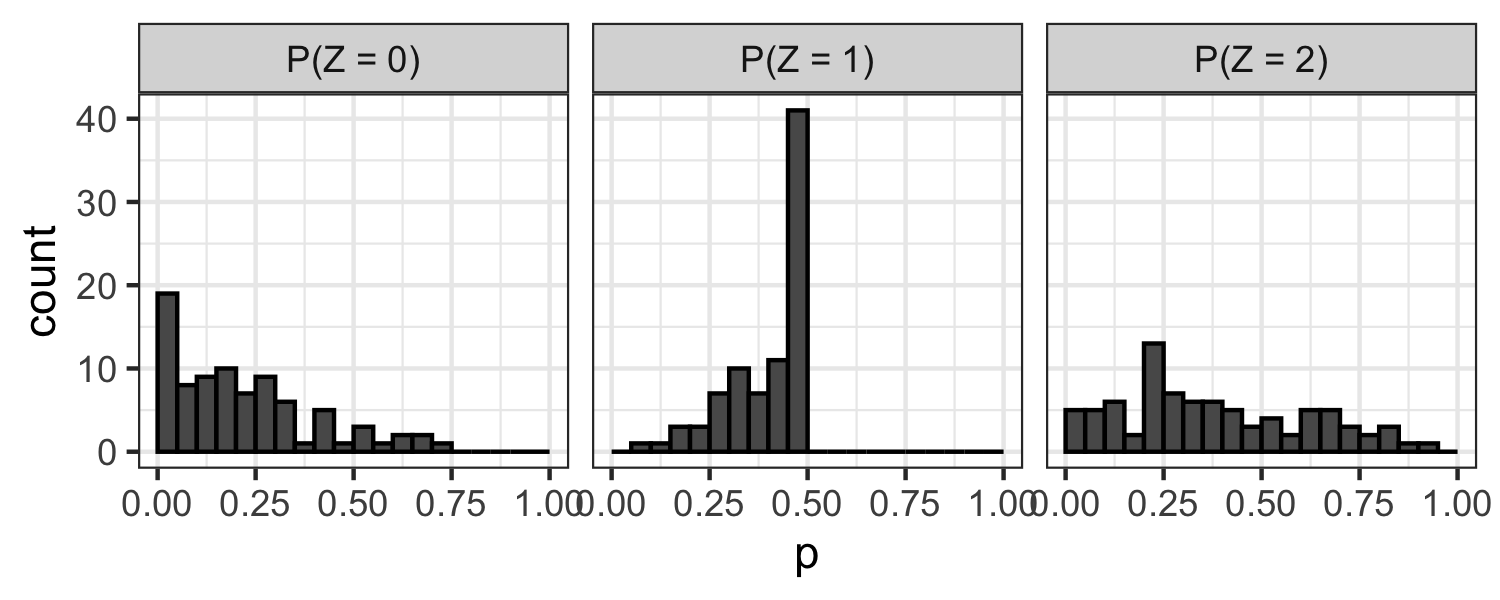
\includegraphics[width = \textwidth]{/Users/ralphtrane/Documents/RPackages_dev/ACEBounds/figures/example_analyses/smoking_depression_marginal_Z.png}
  \caption{Histograms of the marginal distribution of instruments, $P(Z = z), z=0,1,2$, estimated after preprocessing for analysis in Section \ref{smoking-effect-on-depression}}
  \label{fig:marginal-distribution-of-instruments-depression}
\end{figure}

\begin{table}[H]
  \caption{Table of the marginal distribution of instruments, $P(Z = z), z=0,1,2$, estimated after preprocessing for analysis in Section    \ref{smoking-effect-on-depression}}
  \label{tab:marginal-distribution-of-instruments-depression}
  \begin{minipage}{0.5\linewidth}
    \center
    \begin{table}[H]
\centering
\begin{tabular}{lrrr}
\toprule
SNP & P(Z = 2) & P(Z = 1) & P(Z = 0)\\
\midrule
rs10173733 & 0.3567595 & 0.4810680 & 0.1621726\\
rs10193706 & 0.2250921 & 0.4986932 & 0.2762147\\
rs10233018 & 0.2456177 & 0.4999613 & 0.2544211\\
rs10274594 & 0.2534258 & 0.4999767 & 0.2465975\\
rs1029986 & 0.1723555 & 0.4856034 & 0.3420411\\
\addlinespace
rs10774625 & 0.2452793 & 0.4999550 & 0.2547657\\
rs10813628 & 0.2353130 & 0.4995554 & 0.2651316\\
rs10897561 & 0.4145906 & 0.4585930 & 0.1268164\\
rs10905461 & 0.0653045 & 0.3804860 & 0.5542095\\
rs10914684 & 0.4568603 & 0.4381082 & 0.1050314\\
\addlinespace
rs10956808 & 0.3341139 & 0.4878239 & 0.1780622\\
rs11103667 & 0.6529965 & 0.3101710 & 0.0368325\\
rs11127913 & 0.3714083 & 0.4760490 & 0.1525428\\
rs11429972 & 0.1121109 & 0.4454375 & 0.4424516\\
rs11611651 & 0.8320219 & 0.1602609 & 0.0077172\\
\addlinespace
rs11631530 & 0.7776549 & 0.2083850 & 0.0139600\\
rs11646575 & 0.3152078 & 0.4924518 & 0.1923404\\
rs11693702 & 0.2857164 & 0.4976161 & 0.2166675\\
rs117435980 & 0.6997059 & 0.2735567 & 0.0267374\\
rs12042107 & 0.2018720 & 0.4948594 & 0.3032687\\
\addlinespace
rs12244388 & 0.4406271 & 0.4463408 & 0.1130321\\
rs12450028 & 0.4295142 & 0.4517182 & 0.1187675\\
rs12479064 & 0.6269478 & 0.3297051 & 0.0433471\\
rs12487411 & 0.2787537 & 0.4984352 & 0.2228111\\
rs12608052 & 0.2309196 & 0.4992427 & 0.2698378\\
\addlinespace
rs12725407 & 0.6539829 & 0.3094184 & 0.0365987\\
rs12886628 & 0.1122813 & 0.4456055 & 0.4421132\\
rs12910916 & 0.6211224 & 0.3339816 & 0.0448960\\
rs13100688 & 0.3932586 & 0.4676895 & 0.1390519\\
rs1492546 & 0.2020165 & 0.4948919 & 0.3030915\\
\addlinespace
rs1499982 & 0.0222374 & 0.2537694 & 0.7239932\\
rs1549213 & 0.1277548 & 0.4593465 & 0.4128986\\
rs1561195 & 0.2282248 & 0.4990080 & 0.2727672\\
rs1565735 & 0.6370613 & 0.3221998 & 0.0407389\\
rs16951001 & 0.3381946 & 0.4867008 & 0.1751046\\
\addlinespace
rs17003752 & 0.7422782 & 0.2385549 & 0.0191668\\
rs17151637 & 0.5169616 & 0.4040776 & 0.0789607\\
rs1899896 & 0.4936293 & 0.4179166 & 0.0884542\\
rs2240294 & 0.3090443 & 0.4937465 & 0.1972092\\
rs2416770 & 0.2198025 & 0.4980570 & 0.2821405\\
\addlinespace
rs264974 & 0.2632013 & 0.4996604 & 0.2371383\\
rs2675609 & 0.1388997 & 0.4675856 & 0.3935147\\
\bottomrule
\end{tabular}
\end{table}


  \end{minipage}
  \qquad
  \begin{minipage}{0.5\linewidth}
    \center
    \begin{table}[H]
\centering
\begin{tabular}{lrrr}
\toprule
SNP & P(Z = 2) & P(Z = 1) & P(Z = 0)\\
\midrule
rs2797116 & 0.5378179 & 0.3910856 & 0.0710965\\
rs2867749 & 0.4635738 & 0.4345775 & 0.1018487\\
rs299688 & 0.0809490 & 0.4071328 & 0.5119182\\
rs326341 & 0.2744742 & 0.4988573 & 0.2266685\\
rs35891966 & 0.8606480 & 0.1341263 & 0.0052257\\
\addlinespace
rs379525 & 0.2693148 & 0.4992814 & 0.2314038\\
rs42417 & 0.0958938 & 0.4275468 & 0.4765594\\
rs4566215 & 0.2180425 & 0.4978154 & 0.2841421\\
rs4910656 & 0.4335363 & 0.4497969 & 0.1166669\\
rs4957528 & 0.0432628 & 0.3294687 & 0.6272685\\
\addlinespace
rs523528 & 0.1717489 & 0.4853542 & 0.3428969\\
rs528301 & 0.2008634 & 0.4946289 & 0.3045076\\
rs55921136 & 0.6345353 & 0.3240838 & 0.0413808\\
rs568599 & 0.2093354 & 0.4963929 & 0.2942717\\
rs5850689 & 0.1341769 & 0.4642495 & 0.4015736\\
\addlinespace
rs60745548 & 0.0747215 & 0.3972616 & 0.5280169\\
rs6141314 & 0.5745378 & 0.3668899 & 0.0585724\\
rs6265 & 0.6582044 & 0.3061871 & 0.0356085\\
rs6433897 & 0.0693904 & 0.3880603 & 0.5425494\\
rs6676022 & 0.7719180 & 0.2133413 & 0.0147407\\
\addlinespace
rs6690680 & 0.7092842 & 0.2658119 & 0.0249040\\
rs6828849 & 0.3390095 & 0.4864715 & 0.1745191\\
rs71550128 & 0.2006117 & 0.4945706 & 0.3048177\\
rs72505558 & 0.3617365 & 0.4794177 & 0.1588458\\
rs72678864 & 0.6820022 & 0.2876641 & 0.0303337\\
\addlinespace
rs7333559 & 0.0438714 & 0.3311672 & 0.6249614\\
rs7451586 & 0.3546216 & 0.4817591 & 0.1636193\\
rs748828 & 0.5136337 & 0.4060975 & 0.0802688\\
rs7528604 & 0.3204723 & 0.4912608 & 0.1882668\\
rs7567570 & 0.0300586 & 0.2866312 & 0.6833102\\
\addlinespace
rs763053 & 0.6007027 & 0.3486949 & 0.0506025\\
rs76608582 & 0.9065935 & 0.0911171 & 0.0022894\\
rs772921 & 0.4307261 & 0.4511423 & 0.1181316\\
rs77878475 & 0.8356274 & 0.1569984 & 0.0073742\\
rs7870475 & 0.2766026 & 0.4986552 & 0.2247422\\
\addlinespace
rs7948789 & 0.3779911 & 0.4736374 & 0.1483715\\
rs883403 & 0.7155911 & 0.2606702 & 0.0237388\\
rs9375371 & 0.5339661 & 0.3935275 & 0.0725064\\
rs9381917 & 0.8061282 & 0.1834365 & 0.0104354\\
rs9423279 & 0.1176593 & 0.4507114 & 0.4316293\\
\addlinespace
rs9487626 & 0.0333177 & 0.2984272 & 0.6682551\\
rs9835772 & 0.5732121 & 0.3677912 & 0.0589967\\
\bottomrule
\end{tabular}
\end{table}


  \end{minipage}
\end{table}

\begin{figure}[H]
  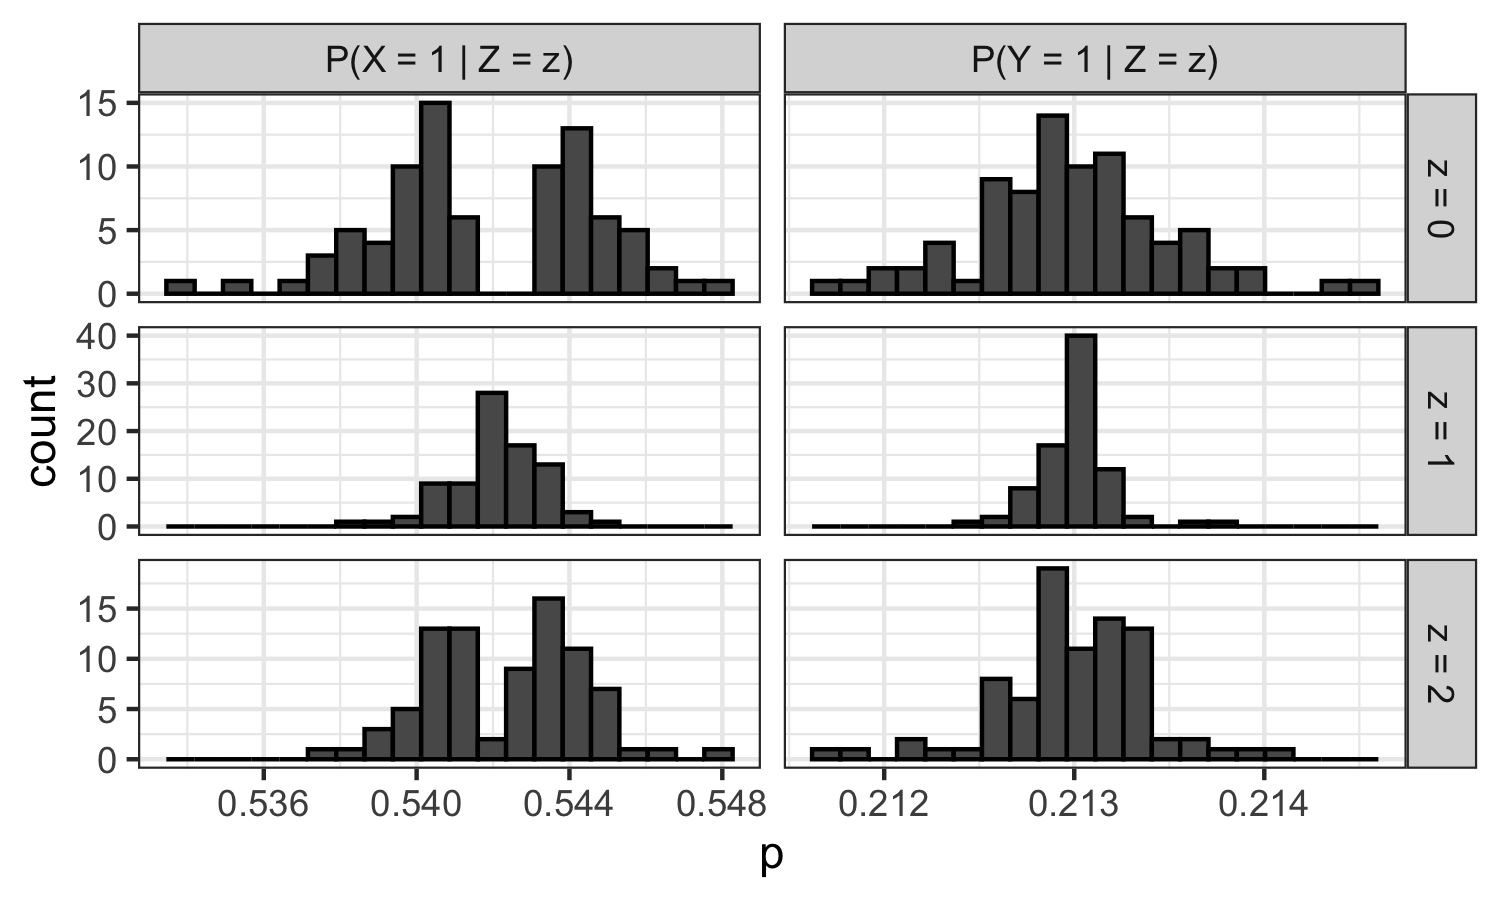
\includegraphics[width = 0.99\linewidth]{/Users/ralphtrane/Documents/RPackages_dev/ACEBounds/figures/example_analyses/smoking_depression_marginal_conditionals.png}
  \caption{Histograms of the marginal conditional probabilities $P(X = 1 | Z = z), z = 0,1,2$ and $P(Y = 1 | Z = z), z=0,1,2$.}
  \label{fig:smoking_on_depression_marginals}
\end{figure}

\begin{figure}[H]
  \center
  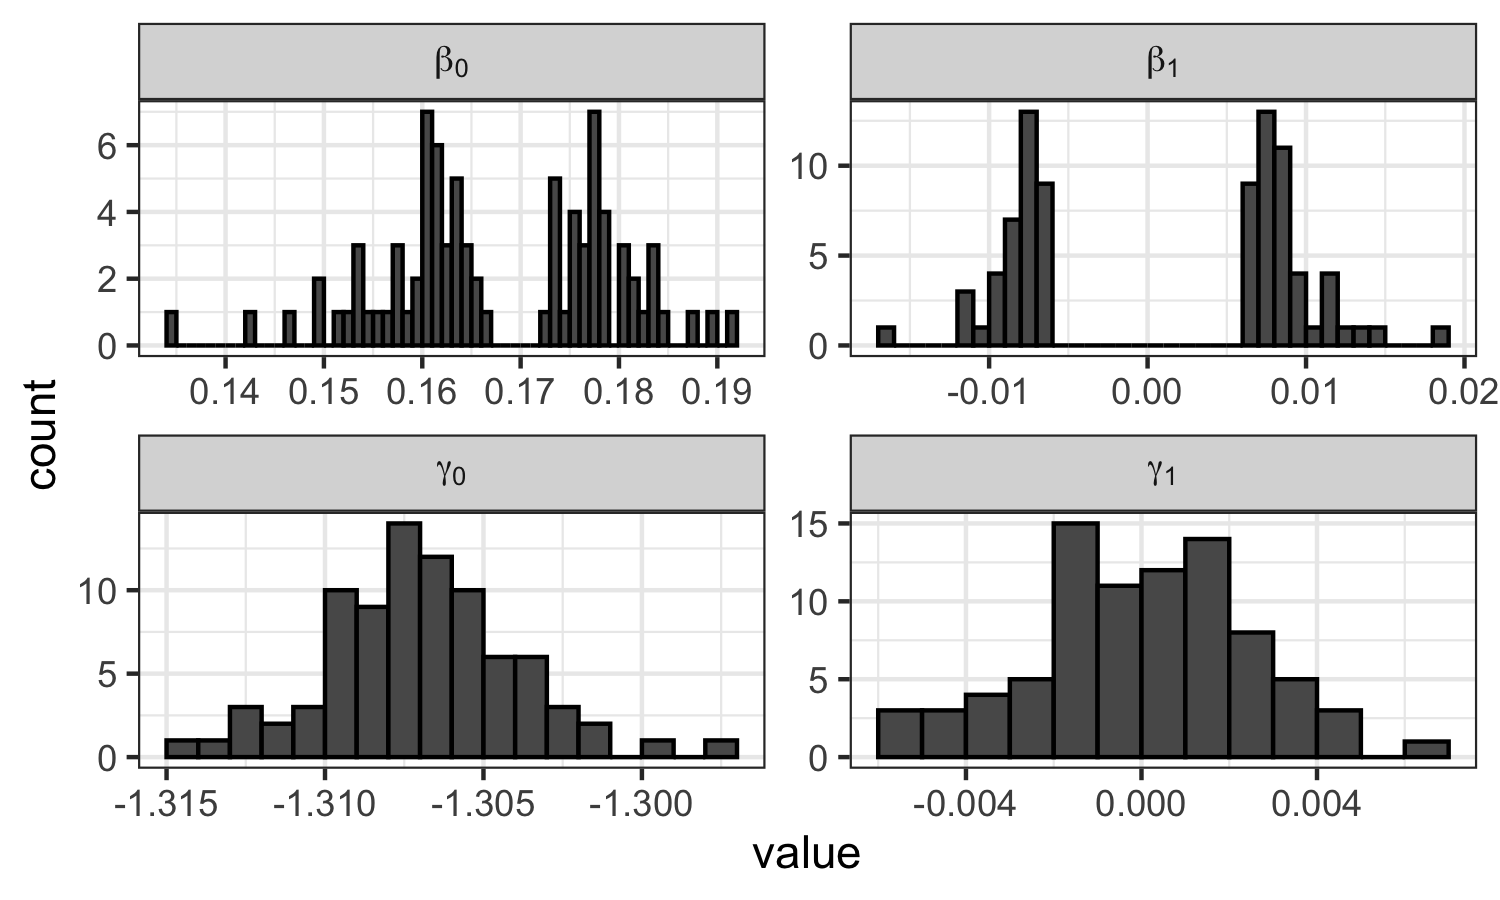
\includegraphics[width = \textwidth]{/Users/ralphtrane/Documents/RPackages_dev/ACEBounds/figures/example_analyses/smoking_depression_coefficients.png}
  \caption{Histograms of the coefficients from GWAS results of logistic regression of the SNPs on smoking status and depression status, respectively. Intercepts ($\beta_0$ and $\gamma_0$) are inferred, while slopes ($\beta_1$ and $\gamma_1$) are as reported.}
  \label{fig:marginal-distribution-of-coefficients-depression}
\end{figure}

\begin{longtable}[t]{lrrrr}
\caption{\label{tab:coefficients-depression}Coefficients from GWAS results of logistic regression of the SNPs on smoking status and depression status. Intercepts ($\beta_0$ and $\gamma_0$) are inferred, while slopes ($\beta_1$ and $\gamma_1$) are as reported.}\\
\toprule
SNP & $\beta_1$ & $\beta_0$ & $\gamma_1$ & $\gamma_0$\\
\midrule
\endfirsthead
\caption[]{\label{tab:coefficients-depression}Coefficients from GWAS results of logistic regression of the SNPs on smoking status and depression status. Intercepts ($\beta_0$ and $\gamma_0$) are inferred, while slopes ($\beta_1$ and $\gamma_1$) are as reported. \textit{(continued)}}\\
\toprule
SNP & $\beta_1$ & $\beta_0$ & $\gamma_1$ & $\gamma_0$\\
\midrule
\endhead

\endfoot
\bottomrule
\endlastfoot
rs10173733 & -0.0065148 & 0.1773825 & -0.0005704 & -1.306311\\
rs10193706 & -0.0117667 & 0.1807672 & 0.0013967 & -1.308318\\
rs10233018 & -0.0076551 & 0.1771881 & 0.0067789 & -1.313719\\
rs10274594 & 0.0078326 & 0.1617143 & 0.0012819 & -1.308284\\
rs1029986 & -0.0070208 & 0.1754296 & 0.0045713 & -1.310792\\
\addlinespace
rs10774625 & 0.0074868 & 0.1621846 & -0.0006839 & -1.306315\\
rs10813628 & -0.0068761 & 0.1762712 & 0.0027284 & -1.309641\\
rs10897561 & -0.0066917 & 0.1782175 & 0.0016886 & -1.309168\\
rs10905461 & 0.0072731 & 0.1658828 & -0.0032370 & -1.305339\\
rs10914684 & 0.0077356 & 0.1591430 & -0.0011037 & -1.305501\\
\addlinespace
rs10956808 & 0.0076247 & 0.1607859 & 0.0000764 & -1.307081\\
rs11103667 & -0.0086047 & 0.1835067 & 0.0046866 & -1.314570\\
rs11127913 & 0.0081801 & 0.1596300 & 0.0021709 & -1.309640\\
rs11429972 & 0.0083148 & 0.1640324 & -0.0016042 & -1.305919\\
rs11611651 & -0.0119868 & 0.1914677 & 0.0004842 & -1.307876\\
\addlinespace
rs11631530 & -0.0099863 & 0.1872129 & -0.0044324 & -1.299176\\
rs11646575 & -0.0082446 & 0.1788582 & 0.0009492 & -1.308059\\
rs11693702 & -0.0080254 & 0.1781801 & 0.0020852 & -1.309223\\
rs117435980 & -0.0092037 & 0.1849976 & -0.0005583 & -1.306059\\
rs12042107 & 0.0071759 & 0.1631519 & 0.0017794 & -1.308592\\
\addlinespace
rs12244388 & -0.0104344 & 0.1834539 & -0.0006776 & -1.306093\\
rs12450028 & -0.0070626 & 0.1788573 & -0.0010781 & -1.305580\\
rs12479064 & -0.0080362 & 0.1823262 & 0.0003346 & -1.307523\\
rs12487411 & 0.0075048 & 0.1616757 & -0.0035878 & -1.303206\\
rs12608052 & 0.0067542 & 0.1631088 & -0.0003997 & -1.306609\\
\addlinespace
rs12725407 & 0.0081386 & 0.1564368 & -0.0012532 & -1.304966\\
rs12886628 & -0.0071010 & 0.1743590 & 0.0007171 & -1.307473\\
rs12910916 & -0.0090138 & 0.1838081 & 0.0029727 & -1.311680\\
rs13100688 & 0.0072663 & 0.1604867 & -0.0026558 & -1.303662\\
rs1492546 & -0.0068801 & 0.1757849 & -0.0005566 & -1.306493\\
\addlinespace
rs1499982 & -0.0114648 & 0.1730198 & 0.0012934 & -1.307379\\
rs1549213 & 0.0085270 & 0.1635050 & -0.0050107 & -1.303414\\
rs1561195 & -0.0078947 & 0.1771435 & 0.0015938 & -1.308516\\
rs1565735 & 0.0115901 & 0.1510995 & 0.0017941 & -1.309857\\
rs16951001 & -0.0066035 & 0.1772805 & 0.0019827 & -1.309300\\
\addlinespace
rs17003752 & 0.0098606 & 0.1526093 & 0.0003979 & -1.307678\\
rs17151637 & 0.0075112 & 0.1587990 & 0.0038108 & -1.312475\\
rs1899896 & -0.0079928 & 0.1808315 & 0.0040686 & -1.312712\\
rs2240294 & 0.0069566 & 0.1618656 & -0.0015763 & -1.305240\\
rs2416770 & -0.0064888 & 0.1756844 & 0.0016061 & -1.308499\\
\addlinespace
rs264974 & 0.0093111 & 0.1600472 & -0.0048647 & -1.302004\\
rs2675609 & 0.0081586 & 0.1635192 & -0.0005645 & -1.306572\\
rs2797116 & 0.0079136 & 0.1579931 & -0.0039810 & -1.301155\\
rs2867749 & 0.0069446 & 0.1601434 & 0.0030286 & -1.311119\\
rs299688 & -0.0072721 & 0.1737381 & 0.0008008 & -1.307449\\
\addlinespace
rs326341 & 0.0065809 & 0.1627046 & -0.0024786 & -1.304396\\
rs35891966 & 0.0147752 & 0.1421862 & -0.0050131 & -1.297691\\
rs379525 & -0.0064906 & 0.1763367 & 0.0020069 & -1.309077\\
rs42417 & -0.0070331 & 0.1739558 & 0.0013904 & -1.307854\\
rs4566215 & 0.0066219 & 0.1634159 & -0.0011016 & -1.305964\\
\addlinespace
rs4910656 & 0.0068438 & 0.1605877 & -0.0003634 & -1.306514\\
rs4957528 & -0.0084750 & 0.1731257 & 0.0023700 & -1.307979\\
rs523528 & 0.0080708 & 0.1629110 & -0.0015950 & -1.305671\\
rs528301 & -0.0086008 & 0.1773101 & -0.0017745 & -1.305403\\
rs55921136 & 0.0085950 & 0.1559070 & -0.0002822 & -1.306543\\
\addlinespace
rs568599 & -0.0067027 & 0.1757335 & 0.0008926 & -1.307810\\
rs5850689 & 0.0119733 & 0.1608303 & -0.0020322 & -1.305504\\
rs60745548 & 0.0071946 & 0.1656667 & -0.0050431 & -1.304238\\
rs6141314 & -0.0080616 & 0.1818212 & 0.0017309 & -1.309617\\
rs6265 & 0.0101598 & 0.1531153 & 0.0034332 & -1.312565\\
\addlinespace
rs6433897 & -0.0072353 & 0.1734119 & 0.0030499 & -1.308601\\
rs6676022 & 0.0115926 & 0.1492301 & 0.0011867 & -1.309078\\
rs6690680 & 0.0088409 & 0.1547086 & -0.0012510 & -1.304886\\
rs6828849 & 0.0067122 & 0.1617838 & -0.0017619 & -1.304941\\
rs71550128 & -0.0073950 & 0.1762247 & 0.0013614 & -1.308213\\
\addlinespace
rs72505558 & 0.0067437 & 0.1614881 & 0.0004530 & -1.307538\\
rs72678864 & 0.0097538 & 0.1534904 & -0.0012454 & -1.304936\\
rs7333559 & 0.0080523 & 0.1662269 & 0.0023047 & -1.307959\\
rs7451586 & -0.0066732 & 0.1775479 & -0.0000777 & -1.306900\\
rs748828 & 0.0086213 & 0.1572430 & -0.0006899 & -1.306004\\
\addlinespace
rs7528604 & 0.0068658 & 0.1618266 & -0.0045708 & -1.301820\\
rs7567570 & -0.0091324 & 0.1727668 & 0.0007640 & -1.307258\\
rs763053 & 0.0080618 & 0.1571035 & -0.0026821 & -1.302836\\
rs76608582 & 0.0182891 & 0.1347725 & 0.0020679 & -1.310931\\
rs772921 & 0.0072725 & 0.1600543 & 0.0018384 & -1.309406\\
\addlinespace
rs77878475 & 0.0125950 & 0.1465734 & -0.0021281 & -1.303102\\
rs7870475 & -0.0071900 & 0.1771631 & 0.0004378 & -1.307453\\
rs7948789 & -0.0161713 & 0.1894889 & 0.0032357 & -1.310973\\
rs883403 & 0.0094240 & 0.1536561 & -0.0018273 & -1.303901\\
rs9375371 & -0.0073963 & 0.1804094 & -0.0032165 & -1.302293\\
\addlinespace
rs9381917 & 0.0112569 & 0.1493862 & -0.0019346 & -1.303519\\
rs9423279 & 0.0076695 & 0.1643388 & -0.0015234 & -1.305948\\
rs9487626 & 0.0131029 & 0.1648180 & -0.0015171 & -1.306439\\
rs9835772 & -0.0078024 & 0.1814146 & 0.0006795 & -1.308022\\*
\end{longtable}

\begin{figure}[H]
  \center
  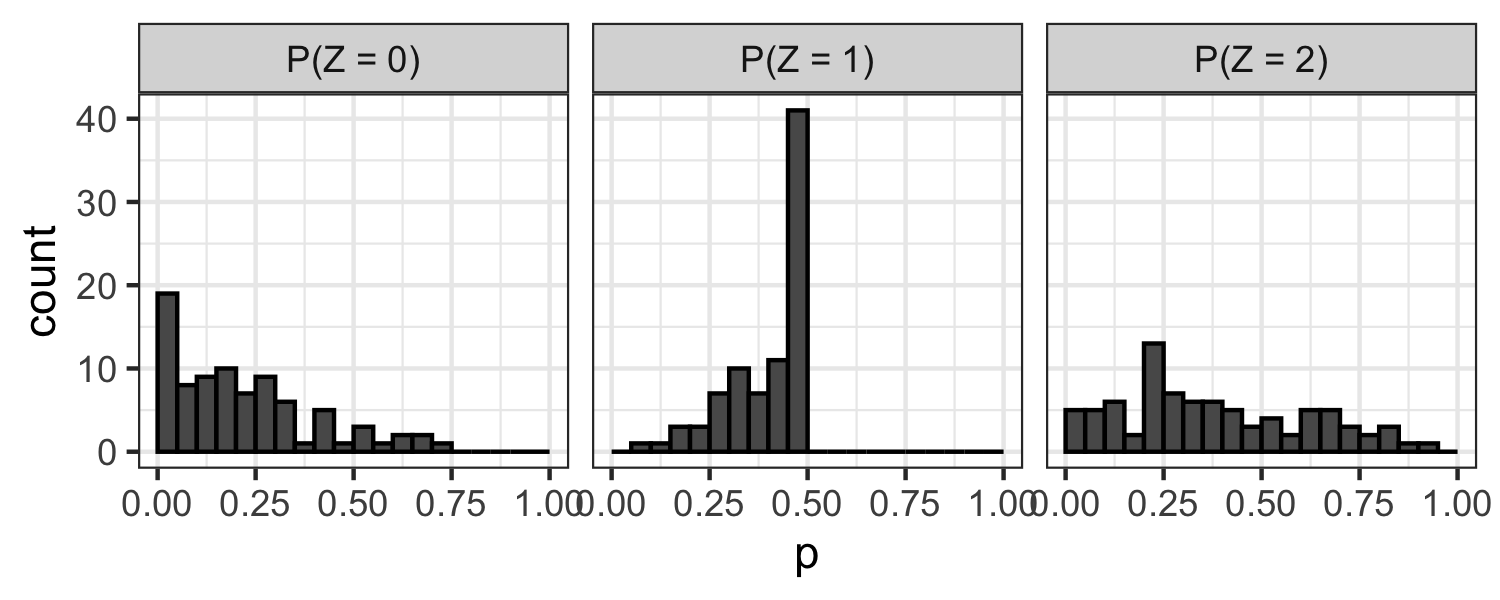
\includegraphics[width = \textwidth]{/Users/ralphtrane/Documents/RPackages_dev/ACEBounds/figures/example_analyses/smoking_lung_cancer_3_marginal_Z.png}
  \caption{Histograms of the marginal distribution of instruments, $P(Z = z), z=0,1,2$, estimated after preprocessing for analysis in Section \ref{smoking-effect-on-lung-cancer}.}
  \label{fig:marginal-distribution-of-instruments-lung-cancer}
\end{figure}

\begin{table}[H]
  \caption{Table of the marginal distribution of instruments, $P(Z = z), z=0,1,2$, estimated after preprocessing for analysis in Section \ref{smoking-effect-on-lung-cancer}}
  \label{tab:marginal-distribution-of-instruments-lung-cancer}
  \begin{minipage}{0.5\linewidth}
    \center
    \begin{table}[H]
\centering
\begin{tabular}{lrrr}
\toprule
SNP & P(Z = 2) & P(Z = 1) & P(Z = 0)\\
\midrule
rs10173733 & 0.3562119 & 0.4812460 & 0.1625421\\
rs10193706 & 0.2254196 & 0.4987283 & 0.2758521\\
rs10233018 & 0.2458307 & 0.4999649 & 0.2542044\\
rs10274594 & 0.2540510 & 0.4999674 & 0.2459816\\
rs1029986 & 0.1723980 & 0.4856208 & 0.3419813\\
\addlinespace
rs10774625 & 0.2457332 & 0.4999633 & 0.2543035\\
rs10813628 & 0.2349574 & 0.4995333 & 0.2655093\\
rs10897561 & 0.4140371 & 0.4588401 & 0.1271228\\
rs10905461 & 0.0654474 & 0.3807590 & 0.5537936\\
rs10914684 & 0.4570550 & 0.4380069 & 0.1049382\\
\addlinespace
rs10956808 & 0.3337643 & 0.4879181 & 0.1783175\\
rs11103667 & 0.6528207 & 0.3103050 & 0.0368743\\
rs11127913 & 0.3717426 & 0.4759287 & 0.1523286\\
rs11429972 & 0.1128192 & 0.4461330 & 0.4410478\\
rs11611651 & 0.8323808 & 0.1599365 & 0.0076827\\
\addlinespace
rs11631530 & 0.7779345 & 0.2081429 & 0.0139226\\
rs11646575 & 0.3149600 & 0.4925059 & 0.1925340\\
rs11693702 & 0.2849095 & 0.4977193 & 0.2173712\\
rs117435980 & 0.6998026 & 0.2734789 & 0.0267185\\
rs12042107 & 0.2025948 & 0.4950210 & 0.3023842\\
\addlinespace
rs12244388 & 0.4404143 & 0.4464457 & 0.1131399\\
rs12450028 & 0.4293549 & 0.4517938 & 0.1188513\\
rs12479064 & 0.6268375 & 0.3297864 & 0.0433761\\
rs12487411 & 0.2788384 & 0.4984262 & 0.2227354\\
rs12608052 & 0.2306302 & 0.4992191 & 0.2701507\\
\addlinespace
rs12725407 & 0.6546886 & 0.3088794 & 0.0364320\\
rs12886628 & 0.1124522 & 0.4457734 & 0.4417744\\
rs12910916 & 0.6206505 & 0.3343265 & 0.0450230\\
rs13100688 & 0.3932914 & 0.4676762 & 0.1390324\\
rs1492546 & 0.2022894 & 0.4949531 & 0.3027575\\
\addlinespace
rs1499982 & 0.0221071 & 0.2531548 & 0.7247382\\
rs1549213 & 0.1285982 & 0.4600154 & 0.4113864\\
rs1561195 & 0.2279701 & 0.4989841 & 0.2730458\\
rs1565735 & 0.6376078 & 0.3217914 & 0.0406009\\
rs16951001 & 0.3380123 & 0.4867519 & 0.1752358\\
\addlinespace
rs17003752 & 0.7420669 & 0.2387323 & 0.0192008\\
rs17151637 & 0.5166809 & 0.4042486 & 0.0790705\\
rs1899896 & 0.4934387 & 0.4180265 & 0.0885349\\
rs2240294 & 0.3093641 & 0.4936820 & 0.1969539\\
rs2416770 & 0.2199058 & 0.4980707 & 0.2820235\\
\addlinespace
rs264974 & 0.2640248 & 0.4996173 & 0.2363579\\
rs2675609 & 0.1387352 & 0.4674731 & 0.3937917\\
\bottomrule
\end{tabular}
\end{table}


  \end{minipage}
  \qquad
  \begin{minipage}{0.5\linewidth}
    \center
    \begin{table}[H]
\centering
\begin{tabular}{lrrr}
\toprule
SNP & P(Z = 2) & P(Z = 1) & P(Z = 0)\\
\midrule
rs2797116 & 0.5370791 & 0.3915554 & 0.0713655\\
rs2867749 & 0.4639468 & 0.4343792 & 0.1016740\\
rs299688 & 0.0806544 & 0.4066855 & 0.5126601\\
rs326341 & 0.2745833 & 0.4988473 & 0.2265693\\
rs35891966 & 0.8609698 & 0.1338295 & 0.0052006\\
\addlinespace
rs379525 & 0.2690001 & 0.4993042 & 0.2316957\\
rs42417 & 0.0959979 & 0.4276747 & 0.4763274\\
rs4566215 & 0.2184561 & 0.4978736 & 0.2836703\\
rs4910656 & 0.4334112 & 0.4498570 & 0.1167317\\
rs4957528 & 0.0432505 & 0.3294341 & 0.6273153\\
\addlinespace
rs523528 & 0.1717181 & 0.4853414 & 0.3429405\\
rs528301 & 0.2006916 & 0.4945891 & 0.3047192\\
rs55921136 & 0.6351822 & 0.3236020 & 0.0412158\\
rs568599 & 0.2090011 & 0.4963306 & 0.2946684\\
rs5850689 & 0.1341980 & 0.4642649 & 0.4015371\\
\addlinespace
rs60745548 & 0.0747101 & 0.3972427 & 0.5280472\\
rs6141314 & 0.5735637 & 0.3675524 & 0.0588839\\
rs6265 & 0.6582586 & 0.3061456 & 0.0355959\\
rs6433897 & 0.0693372 & 0.3879647 & 0.5426982\\
rs6676022 & 0.7713790 & 0.2138057 & 0.0148153\\
\addlinespace
rs6690680 & 0.7094689 & 0.2656618 & 0.0248694\\
rs6828849 & 0.3395694 & 0.4863129 & 0.1741177\\
rs71550128 & 0.2008017 & 0.4946147 & 0.3045837\\
rs72505558 & 0.3617072 & 0.4794276 & 0.1588652\\
rs72678864 & 0.6825787 & 0.2872090 & 0.0302123\\
\addlinespace
rs7333559 & 0.0439935 & 0.3315056 & 0.6245008\\
rs7451586 & 0.3541182 & 0.4819202 & 0.1639616\\
rs748828 & 0.5139770 & 0.4058898 & 0.0801332\\
rs7528604 & 0.3213716 & 0.4910497 & 0.1875787\\
rs7567570 & 0.0299625 & 0.2862686 & 0.6837689\\
\addlinespace
rs763053 & 0.6013164 & 0.3482591 & 0.0504245\\
rs76608582 & 0.9070039 & 0.0907272 & 0.0022689\\
rs772921 & 0.4315416 & 0.4507533 & 0.1177051\\
rs77878475 & 0.8356836 & 0.1569474 & 0.0073690\\
rs7870475 & 0.2763346 & 0.4986816 & 0.2249839\\
\addlinespace
rs7948789 & 0.3767706 & 0.4740916 & 0.1491378\\
rs883403 & 0.7156415 & 0.2606289 & 0.0237296\\
rs9375371 & 0.5345687 & 0.3931467 & 0.0722846\\
rs9381917 & 0.8063218 & 0.1832649 & 0.0104133\\
rs9423279 & 0.1179428 & 0.4509704 & 0.4310869\\
\addlinespace
rs9487626 & 0.0332246 & 0.2981030 & 0.6686724\\
rs9835772 & 0.5737177 & 0.3674477 & 0.0588346\\
\bottomrule
\end{tabular}
\end{table}


  \end{minipage}
\end{table}

\begin{figure}[H]
  \center
  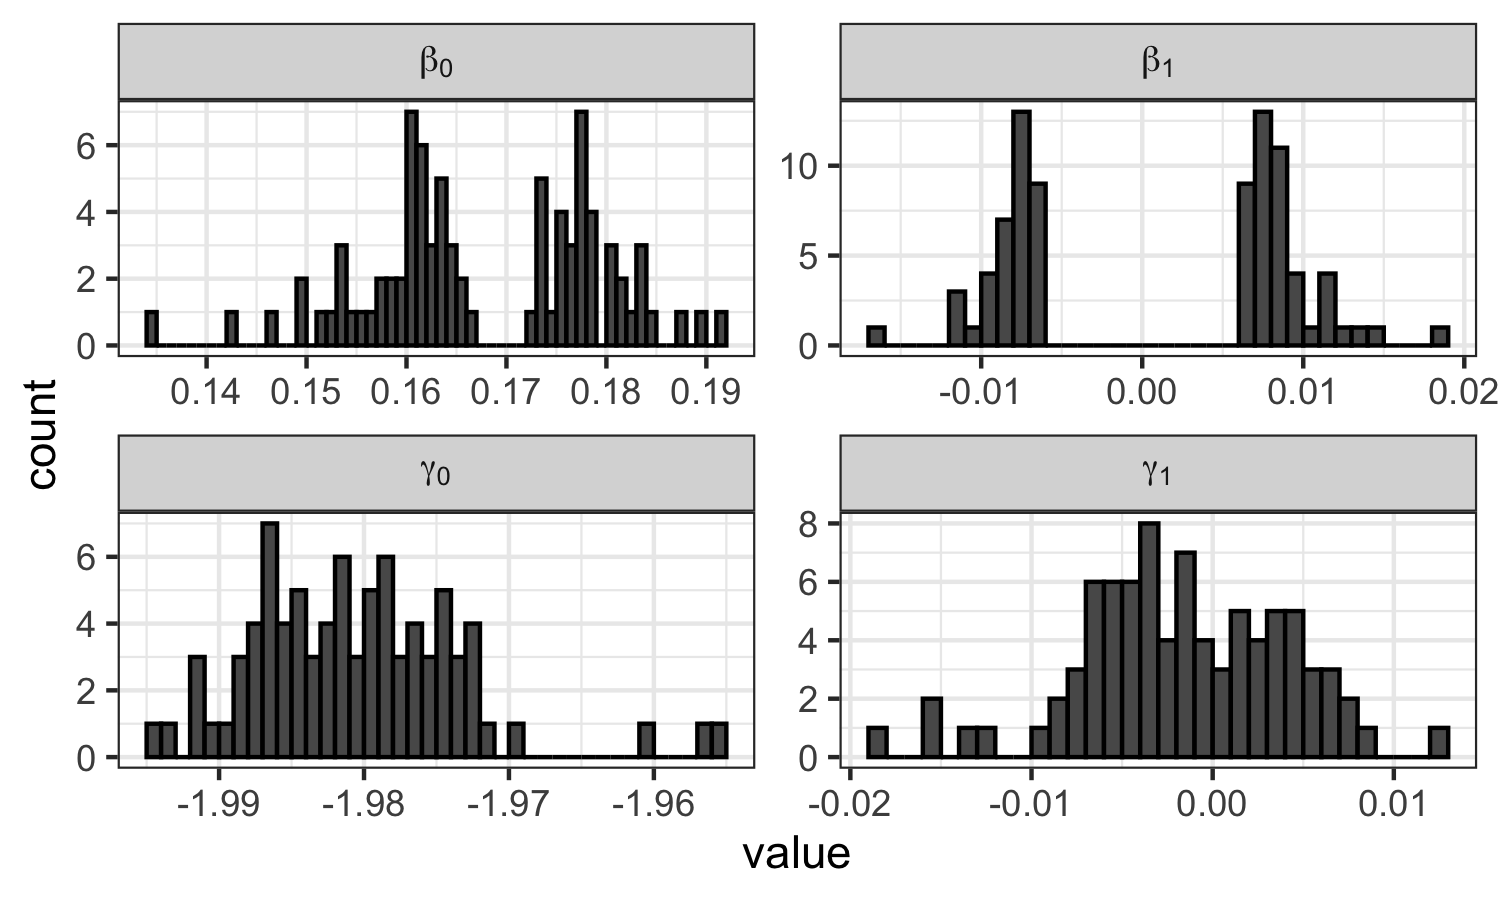
\includegraphics[width = \textwidth]{/Users/ralphtrane/Documents/RPackages_dev/ACEBounds/figures/example_analyses/smoking_lung_cancer_3_coefficients.png}
  \caption{Histograms of the coefficients from GWAS results of logistic regression of the SNPs on smoking status and lung cancer status. Intercepts ($\beta_0$ and $\gamma_0$) are inferred, while slopes ($\beta_1$ and $\gamma_1$) are as reported.}
  \label{fig:marginal-distribution-of-coefficients-lung-cancer}
\end{figure}

\begin{longtable}[t]{lrrrr}
\caption{\label{tab:coefficients-lung-cancer}Coefficients from GWAS results of logistic regression of the SNPs on smoking status and lung cancer status. Intercepts ($\beta_0$ and $\gamma_0$) are inferred, while slopes ($\beta_1$ and $\gamma_1$) are as reported.}\\
\toprule
SNP & $\beta_1$ & $\beta_0$ & $\gamma_1$ & $\gamma_0$\\
\midrule
\endfirsthead
\caption[]{\label{tab:coefficients-lung-cancer}Coefficients from GWAS results of logistic regression of the SNPs on smoking status and lung cancer status. Intercepts ($\beta_0$ and $\gamma_0$) are inferred, while slopes ($\beta_1$ and $\gamma_1$) are as reported. \textit{(continued)}}\\
\toprule
SNP & $\beta_1$ & $\beta_0$ & $\gamma_1$ & $\gamma_0$\\
\midrule
\endhead

\endfoot
\bottomrule
\endlastfoot
rs10173733 & -0.0065148 & 0.1773766 & 0.0033363 & -1.987122\\
rs10193706 & -0.0117667 & 0.1807753 & -0.0015310 & -1.981684\\
rs10233018 & -0.0076551 & 0.1771914 & 0.0050495 & -1.988150\\
rs10274594 & 0.0078326 & 0.1617046 & -0.0015364 & -1.981589\\
rs1029986 & -0.0070208 & 0.1754303 & 0.0035498 & -1.986088\\
\addlinespace
rs10774625 & 0.0074868 & 0.1621777 & -0.0084158 & -1.974806\\
rs10813628 & -0.0068761 & 0.1762662 & 0.0051706 & -1.988156\\
rs10897561 & -0.0066917 & 0.1782117 & 0.0066835 & -1.991747\\
rs10905461 & 0.0072731 & 0.1658787 & -0.0058844 & -1.980131\\
rs10914684 & 0.0077356 & 0.1591408 & -0.0026047 & -1.979616\\
\addlinespace
rs10956808 & 0.0076247 & 0.1607905 & -0.0063546 & -1.975802\\
rs11103667 & -0.0086047 & 0.1835048 & 0.0063118 & -1.993343\\
rs11127913 & 0.0081801 & 0.1596256 & -0.0033969 & -1.978997\\
rs11429972 & 0.0083148 & 0.1640148 & -0.0096129 & -1.976695\\
rs11611651 & -0.0119868 & 0.1914724 & 0.0013059 & -1.985521\\
\addlinespace
rs11631530 & -0.0099863 & 0.1872160 & -0.0047887 & -1.974691\\
rs11646575 & -0.0082446 & 0.1788545 & 0.0012319 & -1.984521\\
rs11693702 & -0.0080254 & 0.1781679 & 0.0046224 & -1.988077\\
rs117435980 & -0.0092037 & 0.1849986 & -0.0054804 & -1.973970\\
rs12042107 & 0.0071759 & 0.1631404 & -0.0020557 & -1.981288\\
\addlinespace
rs12244388 & -0.0104344 & 0.1834505 & 0.0019355 & -1.985707\\
rs12450028 & -0.0070626 & 0.1788556 & -0.0024536 & -1.979923\\
rs12479064 & -0.0080362 & 0.1823251 & -0.0088600 & -1.969116\\
rs12487411 & 0.0075048 & 0.1616745 & -0.0077980 & -1.974913\\
rs12608052 & 0.0067542 & 0.1631129 & -0.0048100 & -1.978521\\
\addlinespace
rs12725407 & 0.0081386 & 0.1564297 & -0.0067998 & -1.972138\\
rs12886628 & -0.0071010 & 0.1743626 & -0.0018595 & -1.981891\\
rs12910916 & -0.0090138 & 0.1838027 & 0.0026458 & -1.987308\\
rs13100688 & 0.0072663 & 0.1604864 & -0.0055464 & -1.976186\\
rs1492546 & -0.0068801 & 0.1757890 & 0.0040638 & -1.986797\\
\addlinespace
rs1499982 & -0.0114648 & 0.1730098 & 0.0024892 & -1.983878\\
rs1549213 & 0.0085270 & 0.1634849 & 0.0056335 & -1.987184\\
rs1561195 & -0.0078947 & 0.1771393 & 0.0072232 & -1.990046\\
rs1565735 & 0.0115901 & 0.1510915 & -0.0072487 & -1.971566\\
rs16951001 & -0.0066035 & 0.1772784 & 0.0070226 & -1.991313\\
\addlinespace
rs17003752 & 0.0098606 & 0.1526117 & -0.0055424 & -1.973591\\
rs17151637 & 0.0075112 & 0.1588020 & -0.0027771 & -1.979146\\
rs1899896 & -0.0079928 & 0.1808293 & 0.0047935 & -1.989876\\
rs2240294 & 0.0069566 & 0.1618616 & -0.0078381 & -1.974429\\
rs2416770 & -0.0064888 & 0.1756858 & -0.0035668 & -1.979794\\
\addlinespace
rs264974 & 0.0093111 & 0.1600323 & -0.0047198 & -1.978291\\
rs2675609 & 0.0081586 & 0.1635228 & -0.0069708 & -1.977953\\
rs2797116 & 0.0079136 & 0.1580011 & -0.0039635 & -1.977330\\
rs2867749 & 0.0069446 & 0.1601396 & -0.0032894 & -1.978658\\
rs299688 & -0.0072721 & 0.1737306 & -0.0019058 & -1.982055\\
\addlinespace
rs326341 & 0.0065809 & 0.1627032 & 0.0031753 & -1.986468\\
rs35891966 & 0.0147752 & 0.1421811 & -0.0122161 & -1.960473\\
rs379525 & -0.0064906 & 0.1763327 & -0.0018594 & -1.981209\\
rs42417 & -0.0070331 & 0.1739582 & 0.0003829 & -1.983375\\
rs4566215 & 0.0066219 & 0.1634100 & -0.0035546 & -1.979817\\
\addlinespace
rs4910656 & 0.0068438 & 0.1605890 & -0.0006962 & -1.982221\\
rs4957528 & -0.0084750 & 0.1731252 & 0.0036288 & -1.984649\\
rs523528 & 0.0080708 & 0.1629116 & 0.0029251 & -1.985564\\
rs528301 & -0.0086008 & 0.1773068 & 0.0124616 & -1.994333\\
rs55921136 & 0.0085950 & 0.1559000 & -0.0069653 & -1.972040\\
\addlinespace
rs568599 & -0.0067027 & 0.1757286 & 0.0043346 & -1.987105\\
rs5850689 & 0.0119733 & 0.1608296 & -0.0038879 & -1.980291\\
rs60745548 & 0.0071946 & 0.1656670 & 0.0062353 & -1.986552\\
rs6141314 & -0.0080616 & 0.1818108 & 0.0010534 & -1.984733\\
rs6265 & 0.0101598 & 0.1531146 & -0.0043806 & -1.976031\\
\addlinespace
rs6433897 & -0.0072353 & 0.1734104 & -0.0011588 & -1.982527\\
rs6676022 & 0.0115926 & 0.1492373 & -0.0153059 & -1.956268\\
rs6690680 & 0.0088409 & 0.1547067 & -0.0050219 & -1.974679\\
rs6828849 & 0.0067122 & 0.1617773 & 0.0008050 & -1.984076\\
rs71550128 & -0.0073950 & 0.1762278 & 0.0034139 & -1.986200\\
\addlinespace
rs72505558 & 0.0067437 & 0.1614885 & -0.0009876 & -1.981950\\
rs72678864 & 0.0097538 & 0.1534836 & -0.0034394 & -1.977455\\
rs7333559 & 0.0080523 & 0.1662222 & -0.0183846 & -1.975467\\
rs7451586 & -0.0066732 & 0.1775422 & 0.0027432 & -1.986404\\
rs748828 & 0.0086213 & 0.1572389 & -0.0047229 & -1.976368\\
\addlinespace
rs7528604 & 0.0068658 & 0.1618157 & -0.0001820 & -1.982931\\
rs7567570 & -0.0091324 & 0.1727617 & -0.0002451 & -1.983053\\
rs763053 & 0.0080618 & 0.1570972 & -0.0069210 & -1.972409\\
rs76608582 & 0.0182891 & 0.1347646 & -0.0048192 & -1.973958\\
rs772921 & 0.0072725 & 0.1600453 & -0.0054837 & -1.975937\\
\addlinespace
rs77878475 & 0.0125950 & 0.1465726 & 0.0010985 & -1.985146\\
rs7870475 & -0.0071900 & 0.1771594 & 0.0082598 & -1.991835\\
rs7948789 & -0.0161713 & 0.1894568 & 0.0009336 & -1.984284\\
rs883403 & 0.0094240 & 0.1536556 & -0.0014726 & -1.980646\\
rs9375371 & -0.0073963 & 0.1804155 & -0.0069852 & -1.972929\\
\addlinespace
rs9381917 & 0.0112569 & 0.1493838 & -0.0155636 & -1.955201\\
rs9423279 & 0.0076695 & 0.1643324 & 0.0046716 & -1.986350\\
rs9487626 & 0.0131029 & 0.1648247 & -0.0136868 & -1.978168\\
rs9835772 & -0.0078024 & 0.1814198 & -0.0031275 & -1.978401\\*
\end{longtable}

\renewcommand\refname{References}
  \bibliography{../references.bib}

\end{document}
